\documentclass[twoside,11pt]{article}
%\documentclass[article,shortnames,nojss]{jss}

\usepackage{jmlr2e}
\usepackage[latin1]{inputenc}
\usepackage[T1]{fontenc}
%\usepackage{times}
%\usepackage[pdftex]{graphicx}
\usepackage{amsmath,amsfonts,amssymb}
\usepackage{bm}
\usepackage{subfigure}
\usepackage{url}
\usepackage{natbib}
\usepackage{longtable}
\usepackage{enumitem}
\usepackage[width=.9\textwidth]{caption}
%\bibliographystyle{plainnat}

\DeclareMathOperator{\Kfu}{\mathbf{K}_{f,u}}
\DeclareMathOperator{\Kuf}{\mathbf{K}_{u,f}}
\DeclareMathOperator{\Kff}{\mathbf{K}_{f,f}}
\DeclareMathOperator{\iKff}{\mathbf{K}_{f,f}^{-1}}
\DeclareMathOperator{\Kfa}{\mathbf{K}_{f,\tilde{f}}}
\DeclareMathOperator{\Kaf}{\mathbf{K}_{\tilde{f},f}}
\DeclareMathOperator{\Kaa}{\mathbf{K}_{\tilde{f},\tilde{f}}}
\DeclareMathOperator{\Kuu}{\mathbf{K}_{u,u}}
\DeclareMathOperator{\iKuu}{\mathbf{K}_{u,u}^{-1}}
\DeclareMathOperator{\Kau}{\mathbf{K}_{\tilde{f},u}}
\DeclareMathOperator{\Kua}{\mathbf{K}_{u,\tilde{f}}}
\DeclareMathOperator{\Qff}{\mathbf{Q}_{f,f}}
\DeclareMathOperator{\Qaa}{\mathbf{Q}_{\tilde{f},\tilde{f}}}
\DeclareMathOperator{\Qfa}{\mathbf{Q}_{f,\tilde{f}}}
\DeclareMathOperator{\Qaf}{\mathbf{Q}_{\tilde{f},f}}
\DeclareMathOperator{\x}{\mathbf{x}}
\DeclareMathOperator{\f}{\mathbf{f}}
\DeclareMathOperator{\y}{\mathbf{y}}
\DeclareMathOperator{\h}{\mathbf{h}}
\DeclareMathOperator{\uu}{\mathbf{u}}
\DeclareMathOperator{\LL}{\mathbf{\Lambda}}
\DeclareMathOperator{\bb}{\mathbf{b}}
\def\WAIC{\mathrm{WAIC}}

\DeclareMathOperator{\Poisson}{Poisson}
\DeclareMathOperator{\NegBin}{NegBin}
\DeclareMathOperator{\Chi}{Chi}
\DeclareMathOperator{\GP}{\mathcal{GP}}
\DeclareMathOperator{\N}{N}
\DeclareMathOperator{\KL}{KL}

\DeclareMathOperator*{\argmax}{arg\,max}
\DeclareMathOperator*{\argmin}{arg\,min}
\newcommand{\mb}{\mathbf}
\newcommand{\pkg}[1]{{\fontseries{b}\selectfont #1}}
\newcommand{\proglang}{}
\newcommand{\email}[1]{\href{mailto:#1}{\normalfont\texttt{#1}}}
\newcommand{\doi}[1]{\href{http://dx.doi.org/#1}{\normalfont\texttt{doi:#1}}}
\newcommand{\code}[1]{{\normalfont\texttt{#1}}}

\DeclareMathOperator{\E}{E}
\DeclareMathOperator{\VAR}{Var}
\DeclareMathOperator{\COV}{Cov}
\DeclareMathOperator{\Prob}{P}

\hyphenation{Veh-ta-ri}

\makeatletter
\def\@oddhead{}%
\def\@oddfoot{}%
\def\@evenhead{}%
\def\@evenfoot{}%
\def\@starteditor{}%
\makeatother
\editor{}
\setlength\aftermaketitskip{0.1in}

%\def\@maketitle{\vbox{\hsize\textwidth
% \linewidth\hsize \vskip \beforetitskip
% {\begin{center} \Large\bf \@title \par \end{center}} \vskip \aftertitskip
% {\def\and{\unskip\enspace{\rm and}\enspace}%
%  \def\addr{\small\it}%
%  \def\email{\hfill\small\sc}%
%  \def\name{\normalsize\bf}%
%  \def\AND{\@endauthor\rm\hss \vskip \interauthorskip \@startauthor}
%  \@startauthor \@author \@endauthor}

%}}

% Link coloring
\usepackage{hyperref}
\hypersetup{
    bookmarks=true,         % show bookmarks bar?
    pdfstartview={FitH},    % fits the width of the page to the window
    colorlinks=true,        % false: boxed links; true: colored links
    linkcolor=black,        % color of internal links
    citecolor=black,        % color of links to bibliography
    filecolor=black,        % color of file links
    urlcolor=black          % color of external links
}

\begin{document}

\title{Bayesian Modeling with Gaussian Processes using the
   \pkg{GPstuff} Toolbox}

\date{2014}

\author{\name Jarno Vanhatalo\thanks{Work done mainly while at the
    Department of Biomedical
    Engineering and Computational Science, Aalto University} \email jarno.vanhatalo@helsinki.fi \\
  \addr Department of Environmental Sciences\\
  University of Helsinki\\
  P.O. Box 65, FI-00014 Helsinki, Finland \AND
  \name Jaakko Riihim\"aki\thanks{Not anymore in Aalto University} \email { } \\
  \name Jouni Hartikainen$^{\dagger}$ \email { } \\
  \name Pasi Jyl\"anki$^{\dagger}$ \email { } \\
  \name Ville Tolvanen \email ville.tolvanen@aalto.fi \\
  \name Aki Vehtari\thanks{Corresponding author} \email aki.vehtari@aalto.fi \\
  \addr Department of Biomedical Engineering and Computational Science\\
  Aalto University School of Science\\
  P.O. Box 12200, FI-00076 Aalto, Finland}
%\author{Jarno Vanhatalo, Jaakko Riihim{\"a}ki, Jouni Hartikainen, Pasi Jyl{\"a}nki,
%  Ville Tolvanen and Aki Vehtari}
%\author{Jarno Vanhatalo\\University of Helsinki\\Aalto University
%  \And Jaakko Riihim{\"a}ki \\ Aalto University \And Jouni Hartikainen
%  \\ Aalto University \And Pasi Jyl{\"a}nki \\ Aalto University \And
%  Ville Tolvanen \\Aalto University \And Aki Vehtari \\Aalto University}

\maketitle

\begin{abstract}%   <- trailing '%' for backward compatibility of .sty file
  Gaussian processes (GP) are powerful tools for probabilistic
  modeling purposes. They can be used to define prior distributions
  over latent functions in hierarchical Bayesian models. The prior
  over functions is defined implicitly by the mean and covariance
  function, which determine the smoothness and variability of the
  function. The inference can then be conducted directly in the
  function space by evaluating or approximating the posterior process.
  Despite their attractive theoretical properties GPs provide
  practical challenges in their implementation. \pkg{GPstuff} is a
  versatile collection of computational tools for GP models compatible
  with Linux and Windows \proglang{MATLAB} and Octave.  It includes,
  among others, various inference methods, sparse approximations and
  tools for model assessment. In this work, we review these tools and
  demonstrate the use of \pkg{GPstuff} in several models.\\ Last updated 2014-04-11.
\end{abstract}

\begin{keywords}
Gaussian process, Bayesian hierarchical model, nonparametric Bayes
\end{keywords}

% \\
% 

\newpage

\tableofcontents

\section{Introduction}

This work reviews a free open source toolbox \pkg{GPstuff} (version
4.4) which implements a collection of inference methods and tools for
inference for various Gaussian process (GP) models. The toolbox is
compatible with Unix and Windows \proglang{MATLAB} \citep{MATLAB:2010}
(r2009b or later, earlier versions may work, but has not been tested
extensively) and \proglang{Octave} \citep{octave:2012} (3.6.4 or
later, compact support covariance functions are not currently working
in Octave). It is available from
\url{http://becs.aalto.fi/en/research/bayes/gpstuff/}.
If you find GPstuff useful, please use the reference \citep{Vanhatalo+gpstuff:2013}
\begin{itemize}
\item[] Jarno Vanhatalo, Jaakko Riihim{\"a}ki, Jouni Hartikainen, Pasi
  Jyl{\"a}nki, Ville Tolvanen and Aki Vehtari (2013). GPstuff: Bayesian
  Modeling with Gaussian Processes. \emph{Journal of Machine Learning
    Research}, 14:1175-1179
\end{itemize}
and appropriate references mentioned in this text or in the GPstuff
functions you are using.

GP is a stochastic process, which provides a powerful tool for
probabilistic inference directly on distributions over functions
\citep[e.g.][]{OHagan:1978} and which has gained much attention in
recent years \citep[][]{Rasmussen+Williams:2006}. In many practical GP
models, the observations $\y = [y_1,...,y_n]^{\text{T}}$ related to
inputs (covariates) $\mb{X} = \{\x_i = [x_{i,1},...
,x_{i,d}]^{\text{T}} \}_{i=1}^n$ are assumed to be conditionally
independent given a latent function (or predictor) $f(\x)$ so that the
likelihood $p(\y|\f) = \prod_{i=1}^{n} p(y_i|f_i)$, where $\f =
[f(\x_1),...,f(\x_n)]^{\text{T}}$, factorizes over cases. GP prior is
set for the latent function after which the posterior $p(f|\y,\mb{X})$
is solved and used for prediction. GP defines the prior over the
latent function implicitly through the mean and covariance function,
which determine, for example, the smoothness and variability of the
latent function.  Usually, the model hierarchy is extended to the
third level by giving also prior for the parameters of the covariance
function and the observation model.

Most of the models in \pkg{GPstuff} follow the above definition and
can be summarized as:
%
\begin{align}
  \text{Observation model:}   &&  \y|\f,\phi   &\sim  \prod_{i=1}^{n} p(y_i|f_i, \phi) \label{likelihood}\\
  \text{GP prior:}   && f(\x)|\theta    &\sim  \GP\left(m(\x),  k(\x,\x'|\theta)\right) \label{GP_prior} \\
  \text{hyperprior:}   &&  \theta, \phi  &\sim  p(\theta)p(\phi). \label{hyper_prior}
\end{align}
%
Here $\theta$ denotes the parameters in the covariance function
$k(\x,\x'|\theta)$, and $\phi$ the parameters in the observation
model. We will call the function value $f(\x)$ at fixed $\x$ a latent
variable and for brevity we sometimes denote all the covariance
function and observation model parameters with $\vartheta = [\theta,
\phi]$. For the simplicity of presentation the mean function is
considered zero, $m(\x) \equiv 0$, throughout this paper. We will also
denote both the observation model and likelihood by $p(\y|\f,\phi)$
and assume the reader is able to distinguish between these two from
the context. The likelihood naming convention is used in the toolbox
for both likelihood and observation model related functionalities
which follows the naming convention used, for example, in \pkg{INLA}
\citep{Rue+Martino+Chopin:2009} and \pkg{GPML}
\citep{Rasmussen+Nickisch:2010} software packages. There are also
models with multiple latent processes and likelihoods where each
factor depens on multiple latent values. These are discussed in
Section \ref{sec:multilatent-models}.

% Many GP models such as general dynamic linear models and multi-output
% models, do not fulfill the assumptions
% \eqref{likelihood}-\eqref{hyper_prior}.  However, the current
% implementation of \pkg{GPstuff} relies on them and as will be seen,
% the class of models fulfilling these assumptions is rather rich. Even
% though the observations are assumed to be conditionally independent
% given the latent variables, the dependencies between the observations
% are incorporated into the model via the GP prior. At the moment, only
% independent priors on $\theta$ and $\phi$ are provided, as highlighted
% by equation \eqref{hyper_prior}, but general form $p(\theta,\phi)$
% could be used as well.
%\pkg{GPstuff} contains one model not fulfilling the general model
%definition, the multi-class model (see \code{demo_multiclass} in the
%package), which has special implementation discussed in
%\citep{Rasmussen+Williams:2006}.

Early examples of GP models can be found, for example, in time series
analysis and filtering \citep{Wiener:1949} and in geostatistics
\citep[e.g.][]{Matheron:1973}.  GPs are still widely used in these
fields and useful overviews are provided in
\citep{Cressie:1993,Grewal+Andrews:2001,Diggle+Ribeiro:2007,Gelfand+Diggle+Fuentes+Guttorp:2010}.
\citet{OHagan:1978} was one of the firsts to consider GPs in a general
probabilistic modeling context and provided a general theory of GP
prediction. This general regression framework was later rediscovered
as an alternative for neural network models
\citep{Williams+Rasmussen:1996,Rasmussen:1996} and extended for other
problems than regression \citep{Neal:1997,Williams+Barber:1998}. This
machine learning perspective is comprehensively summarized by
\citet{Rasmussen+Williams:2006}.

Nowadays, GPs are used, for example, in weather forecasting
\citep{Fuentes+Raftery:2005,Berrocal+Raftery+Gneiting+Steed:2009},
spatial statistics
\citep{Best+Richardson+Thomson:2005,Kaufman+Schervish+Nychka:2008,Banerjee+Gelfand+Finley+Sang:2008,Myllymaki+Sarkka+Vehtari:2014},
computational biology
\citep{Honkela+Gao+Ropponen+Rattray+Lawrence:2011}, reinforcement
learning
\citep{Deisenroth+Rasmussen+Peters:2009,Deisenroth+Rasmussen+Fox:2011},
healthcare applications
\citep{Stegle+Fallert+MacKay+Brage:2008,Vanhatalo+Pietilainen+Vehtari:2010,Rantonen+Vehtari+etal:2012,Rantonen+Vehtari+etal:2014},
survival analysis \citep{Joensuu+etal:2012a,Joensuu+Reichardt+Eriksson+Hall+Vehtari:2014}
industrial applications \citep{Kalliomaki+Vehtari+Lampinen:2005},
computer model calibration and emulation
\citep{Kennedy+OHagan:2001,Conti+Gosling+Oakley+OHagan:2009}, prior
elicitation \citep{Moala+OHagan:2010} and density estimation
\citep{Tokdar+Ghosh:2007,Tokdar+Zhu+Ghosh:2010,Riihimaki+Vehtari:2014} to name a few.
Despite their attractive theoretical properties and wide range of
applications, GPs provide practical challenges in implementation.

\pkg{GPstuff} provides several state-of-the-art inference algorithms
and approximative methods that make the inference easier and faster
for many practically interesting models. \pkg{GPstuff} is a modular
toolbox which combines inference algorithms and model structures in an
easily extensible format. % We have paid attention to a robust
% implementation which is not straightforward with GP models in general.
It also provides various tools for model checking and comparison.
These are essential in making model assessment and criticism an
integral part of the data analysis. Many algorithms and models in
\pkg{GPstuff} are proposed by others but reimplemented for
\pkg{GPstuff}. In each case, we provide reference to the original work
but the implementation of the algorithm in \pkg{GPstuff} is always
unique. The basic implementation of two important algorithms, the
Laplace approximation and expectation propagation algorithm (discussed
in Section \ref{sec_cond_post_of_latent}), follow the pseudocode from
\citep{Rasmussen+Williams:2006}. However, these are later generalized
and improved as described in
\citep{Vanhatalo+Jylanki+Vehtari:2009,Vanhatalo+Pietilainen+Vehtari:2010,
  Vanhatalo+Vehtari:2010,Jylanki+Vanhatalo+Vehtari:2011,Riihimaki+Jylanki+Vehtari:2013,Riihimaki+Vehtari:2014}.

There are also many other toolboxes for GP modelling than
\pkg{GPstuff} freely available. Perhaps the best known packages are
nowadays the Gaussian processes for Machine Learning \pkg{GPML}
toolbox \citep{Rasmussen+Nickisch:2010} and the flexible Bayesian
modelling (\pkg{FBM}) toolbox by Radford Neal. A good overview of
other packages can be obtained from the Gaussian processes website
\url{http://www.gaussianprocess.org/} and the \proglang{R} Archive
Network \url{http://cran.r-project.org/}.  Other GP softwares have
some overlap with \pkg{GPstuff} and some of them include models that
are not implemented in \pkg{GPstuff}.  The main advantages of
\pkg{GPstuff} over other GP software are its versatile collection of
models and computational tools as well as modularity which allows easy
extensions. A comparison between \pkg{GPstuff}, \pkg{GPML} and
\pkg{FBM} is provided in the Appendix \ref{appendix:comparison}.

Three earlier GP and Bayesian modelling packages have influenced our
work.  Structure of \pkg{GPstuff} is mostly in debt to the
\pkg{Netlab} toolbox \citep{Nabney:2001}, although it is far from
being compatible.  The \pkg{GPstuff} project was started in 2006 based on
the \pkg{MCMCStuff}-toolbox (1998-2006)
(\url{http://becs.aalto.fi/en/research/bayes/mcmcstuff/}). \pkg{MCMCStuff}
for its part was based on \pkg{Netlab} and it was also influenced by
the \pkg{FBM}. The \pkg{INLA} software package by
\citet{Rue+Martino+Chopin:2009} has also motivated some of the
technical details in the toolbox. In addition to these, some technical
implementations of \pkg{GPstuff} rely on the sparse matrix toolbox
\pkg{SuiteSparse} \citep{Davis:2005}
(\url{http://www.cise.ufl.edu/research/sparse/SuiteSparse/}).

% This work is organized as follows. First the general form of the
% models in \pkg{GPstuff} is described.  After this in sections
% \ref{sec_cond_post_of_latent} and
% \ref{sec_marginalization_over_hyperparam} the inference techniques
% implemented in \pkg{GPstuff} are introduced in a general level and
% references are given to direct the reader for a more detailed
% discussion on them. Section \ref{chap:intro_to_GPstuff} considers
% simple GP regression and classification problems. These serve as
% examples on how to use functions in \pkg{GPstuff}. After this, we
% introduce the sparse GP models in section \ref{chapter_sparse_GPs} and
% the model assessment methods in section \ref{sec:model_assessment}.
% Sections \ref{sec:modifying_covariance} to
% \ref{sec_adding_new_features} give an overview on how the covariance
% functions can be modified from their default form, introduce rest of
% the observation models and give a short description on how
% \pkg{GPstuff} can be extended. We end with discussion.

% \pkg{GPstuff} can be used to build elaborate hierarchical models and
% prior structures requiring often several lines of code. 

This work concentrates on discussing the essential theory and methods
behind the implementation of \pkg{GPstuff}. We explain important parts
of the code, but the full code demonstrating the important features of
the package (including also data creation and such), are included in
the demonstration files \code{demo\_*} to which we refer in the text.

\section{Gaussian process models}

\subsection{Gaussian process prior}

GP prior over function $f(\x)$ implies that any set of function values
$\f$, indexed by the input coordinates $\mb{X}$, have a multivariate
Gaussian distribution
%
\begin{equation}\label{eq_GP_prior}
p(\f|\mb{X},\theta) = \N(\f|\mb{0}, \Kff),
\end{equation}
% 
where $\Kff$ is the covariance matrix. Notice, that the distribution
over functions will be denoted by $\GP(\cdot,\cdot)$, whereas the
distribution over a finite set of latent variables will be denoted by
$\N(\cdot,\cdot)$. The covariance matrix is constructed by a
covariance function, $[\Kff]_{i,j} = k(\mb{x}_i, \mb{x}_j|\theta)$,
which characterizes the correlation between different points in the
process.  Covariance function can be chosen freely as long as the
covariance matrices produced are symmetric and positive semi-definite
($\mb{v}^{\text{T}}\Kff\mb{v}\geq 0, \forall \mb{v}\in \Re^n$). An
example of a stationary covariance function is the squared exponential
%
\begin{equation}
k_{\mathrm{se}}(\x_i,\x_j|\theta)=\sigma_{\mathrm{se}}^2\exp(-r^2/2),
\end{equation}
%
where $r^2 = \sum_{k=1}^d (x_{i,k}-x_{j,k})^2/l_k^2$ and $\theta =
[\sigma_{\mathrm{se}}^2, l_1,...,l_d]$. Here, $\sigma_{\mathrm{se}}^2$
is the scaling parameter, and $l_k$ is the length-scale, which governs
how fast the correlation decreases as the distance increases in the
direction $k$. Other common covariance functions are discussed, for
example, by \citet{Diggle+Ribeiro:2007},
\citet{Finkenstadt+Held+Isham:2007} and
\citet{Rasmussen+Williams:2006} and the covariance functions in
\pkg{GPstuff} are summarized in the appendix
\ref{covariance_functions}.

Assume that we want to predict the values $\tilde{\f}$ at new input
locations $\tilde{\mb{X}}$. The joint prior for latent variables $\f$
and $\tilde{\f}$ is
%
\begin{equation}
\left[ \begin{matrix} \f \\ \tilde{\f} \end{matrix} \right] | \mb{X},
\tilde{\mb{X}},\theta
\sim \N\left(\mb{0}, \left[ \begin{matrix} \Kff & \Kfa \\ \Kaf & \Kaa
    \end{matrix} \right] \right),
\end{equation}
%
where $\Kff = k(\mb{X},\mb{X}|\theta)$, $\Kfa =
k(\mb{X},\tilde{\mb{X}}|\theta)$ and $\Kaa =
k(\tilde{\mb{X}},\tilde{\mb{X}}|\theta)$. Here, the covariance
function $k(\cdot,\cdot)$ denotes also vector and matrix valued
functions $k(\x,\mb{X}):\Re^d \times \Re^{d \times n}\rightarrow
\Re^{1\times n}$, and $k(\mb{X},\mb{X}):\Re^{d\times n}\times
\Re^{d\times n}\rightarrow \Re^{n\times n}$. By definition of GP the
marginal distribution of $\tilde{\f}$ is
$p(\tilde{\f}|\tilde{\mb{X}},\theta) = \N(\tilde{\f}|\mb{0}, \Kaa)$
similar to \eqref{eq_GP_prior}.  The conditional distribution of
$\tilde{\f}$ given $\f$ is
%
\begin{equation}\label{eq_conditional_ftilde_given_f}
\tilde{\f}|\f, \mb{X},
\tilde{\mb{X}}, \theta \sim \N(\Kaf\iKff\f, \Kaa - \Kaf\iKff\Kfa),
\end{equation}
%
where the mean and covariance of the conditional distribution are
functions of input vector $\tilde{\x}$ and $\mb{X}$ serves as a fixed
parameter.  Thus, the above distribution generalizes to GP with mean
function $m(\tilde{\x}|\theta) = k(\tilde{\x},\mb{X}|\theta)\iKff\f$
and covariance $k(\tilde{\x}, \tilde{\x}'|\theta) = k(\tilde{\x},
\tilde{\x}'|\theta) - k(\tilde{\x},\mb{X}|\theta)\iKff
k(\mb{X},\tilde{\x}'|\theta)$, which define the conditional
distribution of the latent function $f(\tilde{\x})$.

\subsection{Conditioning on the observations}

The cornerstone of the Bayesian inference is Bayes' theorem by
which the conditional probability of the latent function and
parameters after observing the data can be solved. This posterior
distribution contains all information about the latent function and
parameters conveyed from the data $\mathcal{D} = \{\mb{X}, \mb{y}\}$
by the model. Most of the time we cannot solve the posterior but need
to approximate it.  \pkg{GPstuff} is built so that the first inference
step is to form (either analytically or approximately) the conditional
posterior of the latent variables given the parameters 
%
\begin{equation}\label{eq_conditional_posterior_of_f}
p(\f|\mathcal{D}, \theta, \phi) =
\frac{p(\y|\f,\phi)p(\f|,\mb{X}, \theta)}{\int p(\y|\f,\phi)p(\f|\mb{X},\theta) d\f},
\end{equation}
%
which is discussed in the section~\ref{sec_cond_post_of_latent}. After
this, we can (approximately) marginalize over the parameters to obtain the
marginal posterior distribution for the latent variables
%
\begin{equation}
p(\f|\mathcal{D}) = \int p(\f|\mathcal{D}, \theta, \phi) p(\theta, \phi|\mathcal{D}) d\theta d\phi
\end{equation}
%
treated in the section~\ref{sec_marginalization_over_hyperparam}. The
posterior predictive distributions can be obtained similarly by first
evaluating the conditional posterior predictive distribution, for
example $p(\tilde{f}|\mathcal{D}, \theta, \phi, \tilde{\x})$, and then
marginalizing over the parameters. The joint predictive distribution
$p(\tilde{\y}|\mathcal{D}, \theta, \phi, \tilde{\x})$ would require
integration over possibly high dimensional distribution
$p(\tilde{\f}|\mathcal{D}, \theta, \phi, \tilde{\x})$. However,
usually we are interested only on the marginal predictive distribution
for each $\tilde{y}_i$ separately which requires only one dimensional
integrals
%
\begin{equation}
  p(\tilde{y}_i | \mathcal{D}, \tilde{\mb{x}}_i, \theta, \phi) = \int p(\tilde{y_i}|
  \tilde{f}_i, \phi) p(\tilde{f}_i | 
  \mathcal{D}, \tilde{\x}_i, \theta, \phi)d \tilde{f}_i.
\end{equation}

If the parameters are considered fixed, GP's marginalization and
conditionalization properties can be exploited in the prediction.
Given the conditional posterior distribution $p(\f|\mathcal{D},\theta,
\phi)$, which in general is not Gaussian, we can evaluate the
posterior predictive mean from the conditional mean
$\E_{\tilde{\f}|\f,\theta,\phi}[f(\tilde{\x})] =
k(\tilde{\x},\mb{X})\iKff\f$ (see equation
\eqref{eq_conditional_ftilde_given_f} and the text below it). Since
this holds for any $\tilde{\f}$, we obtain a parametric posterior mean
function
%
\begin{eqnarray}\label{eq_posterior_predictive_mean}
m_p(\tilde{\x}|\mathcal{D},\theta,\phi) =
\int \E_{\tilde{\f}|\f,\theta,\phi}[f(\tilde{\x})]
p(\f|\mathcal{D},\theta,\phi) d\f = k(\tilde{\x},\mb{X}|\theta)\iKff
\E_{\f|\mathcal{D},\theta,\phi}[\f]. 
\end{eqnarray}
%
The posterior predictive covariance between any set of latent
variables, $\tilde{\f}$ is 
%
\begin{equation}
\COV_{\tilde{\f}|\mathcal{D},\theta,\phi}[\tilde{\f}] = \E_{\f|\mathcal{D},\theta,\phi}
\left[\COV_{\tilde{\f}|\f}[\tilde{\f}] \right] +
\COV_{\f|\mathcal{D},\theta,\phi}\left[\E_{\tilde{\f}|\f}[\tilde{\f} ]\right],
\end{equation}
%
where the first term simplifies to the conditional covariance in
equation \eqref{eq_conditional_ftilde_given_f} and the second term to
$k(\tilde{\x},\mb{X}) \iKff \COV_{\f|\mathcal{D},\theta,\phi}[\f]\iKff
k(\mb{X},\tilde{\x}')$. The posterior covariance function is then
%
\begin{equation}\label{eq_posterior_predictive_covariance}
% \COV_{\tilde{\f}|\mathcal{D}}[\tilde{\f}] = \Kaa - \Kaf\iKff\Kfa +
% \Kaf\iKff \COV_{\f|\mathcal{D}}[\f]\iKff\Kfa. 
k_p(\tilde{\x},\tilde{\x}'|\mathcal{D},\theta,\phi) = k(\tilde{\x},\tilde{\x}'|\theta) - k(\tilde{\x},\mb{X}|\theta) \left(\iKff -
\iKff \COV_{\f|\mathcal{D},\theta,\phi}[\f]\iKff\right)k(\mb{X},\tilde{\x}'|\theta). 
\end{equation}
%
From now on the posterior predictive mean and covariance will be
denoted $m_p(\tilde{\x})$ and $k_p(\tilde{\x},\tilde{\x}')$.

Even if the exact posterior $p(\tilde{f}|\mathcal{D},\theta,\phi)$ is
not available in closed form, we can still approximate its posterior
mean and covariance functions if we can approximate
$\E_{\f|\mathcal{D},\theta,\phi}$ and
$\COV_{\f|\mathcal{D},\theta,\phi}[\f]$. A common practice to
approximate the posterior $p(\f|\mathcal{D},\theta,\phi)$ is either
with Markov chain Monte Carlo (MCMC)
\citep[e.g.][]{Neal:1997,Neal:1998,Diggle+Tawn+Moyeed:1998,Kuss+Rasmussen:2005,Christensen+Roberts+Skold:2006}
or by giving an analytic approximation to it
\citep[e.g.][]{Williams+Barber:1998,Gibbs+MacKay:2000,Minka:2001,Csato+Opper:2002,Rue+Martino+Chopin:2009}.
The analytic approximations considered here assume a Gaussian form in
which case it is natural to approximate the predictive distribution
with a Gaussian as well.  In this case, the equations
\eqref{eq_posterior_predictive_mean} and
\eqref{eq_posterior_predictive_covariance} give its mean and
covariance. Detailed considerations on the approximation error and the
asymptotic properties of the Gaussian approximation are presented, for
example, by \citet{Rue+Martino+Chopin:2009} and
\citet{Vanhatalo+Pietilainen+Vehtari:2010}.

\section{Conditional posterior and predictive distributions}\label{sec_cond_post_of_latent}

\subsection{Gaussian observation model: the analytically tractable case}
\label{sec:gauss-observ-model}

With a Gaussian observation model, $y_i \sim \N(f_i, \sigma^2)$, where
$\sigma^2$ is the noise variance, the conditional posterior of the
latent variables can be evaluated analytically. Marginalization over
$\f$ gives the marginal likelihood
%
\begin{equation}\label{eq_marginal_likelihood_gaussian_case}
p(\y|\mb{X},\theta, \sigma^2) = \N(\y|\mb{0}, \Kff + \sigma^2\mb{I}).
\end{equation}
%
Setting this in the denominator of the equation
\eqref{eq_conditional_posterior_of_f}, gives a Gaussian distribution
also for the conditional posterior of the latent variables
%
\begin{equation}\label{eq_posterior_in_gaussian_case}
\f|\mathcal{D},\theta, \sigma^2 \sim \N(\Kff(\Kff + \sigma^2\mb{I})^{-1}\y, \Kff - \Kff(\Kff + \sigma^2\mb{I})^{-1}\Kff).
\end{equation}

Since the conditional posterior of $\f$ is Gaussian, the posterior
process, or distribution $p(\tilde{f}|\mathcal{D})$, is also Gaussian.
By placing the mean and covariance from
\eqref{eq_posterior_in_gaussian_case} in the equations
\eqref{eq_posterior_predictive_mean} and
\eqref{eq_posterior_predictive_covariance} we obtain the predictive
distribution
%
\begin{equation}\label{eq_posterior_predictive_in_gaussian_case}
\tilde{f}|\mathcal{D},\theta, \sigma^2 \sim \GP\left(m_{\text{p}}(\tilde{\x}), k_{\text{p}}(\tilde{\x},\tilde{\x}')\right),
% \tilde{\f}|\mathcal{D},\theta, \sigma^2 \sim \N(k(\tilde{\x},\mb{X})(\Kff +
% \sigma^2\mb{I})^{-1}\y, k(\tilde{\x},\tilde{\x}') - k(\tilde{\x},\mb{X})(\Kff + \sigma^2\mb{I})^{-1}k(\mb{X},\tilde{\x})). 
\end{equation}
%
where the mean is $m_{\text{p}}(\tilde{\x}) = k(\tilde{\x},\mb{X})(\Kff +
\sigma^2\mb{I})^{-1}\y$ and covariance is $k_{\text{p}}(\tilde{\x},\tilde{\x}') =k(\tilde{\x},\tilde{\x}') -
k(\tilde{\x},\mb{X})(\Kff +
\sigma^2\mb{I})^{-1}k(\mb{X},\tilde{\x}')$. The predictive
distribution for new observations $\tilde{\y}$ can be obtained by
integrating $p(\tilde{\y}|\mathcal{D},\theta, \sigma^2) = \int
p(\tilde{\y}|\tilde{\f},\sigma^2)p(\tilde{\f}|\mathcal{D},\theta,
\sigma^2)d\tilde{\f}$. The result is, again, Gaussian with mean
$\E_{\tilde{\f}|\mathcal{D},\theta}[\tilde{\f}]$ and covariance
$\COV_{\tilde{\f}|\mathcal{D},\theta}[\tilde{\f}] + \sigma^2\mb{I}$. 

\subsection{Laplace approximation}

With a non-Gaussian likelihood the conditional posterior needs to be
approximated. The Laplace approximation is constructed from the second
order Taylor expansion of $\log p(\f|\y,\theta, \phi)$ around the mode
$\hat{\f}$, which gives a Gaussian approximation to the conditional
posterior
%
\begin{equation}\label{eq_latent_posterior_in_Laplace_case}
p(\f|\mathcal{D},\theta,\phi) \approx q(\f|\mathcal{D},\theta,\phi) =
\N(\f|\hat{\f}, \mb{\Sigma}), 
\end{equation}
%
where $\hat{\f}=\argmax_{\mb{f}} p(\f|\mathcal{D},\theta,\phi)$ and
$\mb{\Sigma}^{-1}$ is the Hessian of the negative log conditional posterior
at the mode \citep{Gelman+etal+BDA3:2013,Rasmussen+Williams:2006}: 
%
\begin{equation}
\mb{\Sigma}^{-1} = -\nabla\nabla \log
p(\f|\mathcal{D},\theta,\phi)|_{\f=\hat{\f}} = \iKff + \mb{W},
\label{Hessian} 
\end{equation}
%
where $\mb{W}$ is a diagonal matrix with entries $\mb{W}_{ii} =
\nabla_{f_i}\nabla_{f_i} \log p(y|f_i,\phi)|_{f_i=\hat{f}_i}$.
%
We call the approximation scheme Laplace method following
\citet{Williams+Barber:1998}, but essentially the same approximation
is named Gaussian approximation by \citet{Rue+Martino+Chopin:2009}.

Setting $\E_{\f|\mathcal{D},\theta}[\f] = \hat{\f}$ and
$\COV_{\f|\mathcal{D},\theta}[\f] = (\iKff + \mb{W})^{-1}$ into
\eqref{eq_posterior_predictive_mean} and
\eqref{eq_posterior_predictive_covariance} respectively, gives after
rearrangements and using $\iKff\hat{\f} = \nabla\log
p(\y|\f)|_{\f=\hat{\f}}$, the approximate posterior predictive
distribution
%
\begin{equation}\label{eq_posterior_in_Laplace_case}
\tilde{f}|\mathcal{D},\theta, \sigma^2 \sim \GP\left(m_{\text{p}}(\tilde{\x}), k_{\text{p}}(\tilde{\x},\tilde{\x}')\right).
\end{equation}
%
Here the mean and covariance are $m_{\text{p}}(\tilde{\x}) = k(\tilde{\x},\mb{X})\nabla\log
p(\y|\f)|_{\f=\hat{\f}}$ and 
$k_{\text{p}}(\tilde{\x},\tilde{\x}')=k(\tilde{\x},\tilde{\x}') - k(\tilde{\x},\mb{X})(\Kff +
\mb{W})^{-1}k(\mb{X},\tilde{\x}')$.
%
The approximate conditional predictive density of $\tilde{y}_i$ can
now be evaluated, for example, with quadrature integration over each
$\tilde{f}_i$ separately
%
\begin{equation}
p(\tilde{y}_i|\mathcal{D}, \theta, \phi) \approx \int
p(\tilde{y}_i|\tilde{f}_i,\phi)q(\tilde{f}_i|\mathcal{D}, \theta,
\phi) d \tilde{f}_i. 
\end{equation}
%    
\subsection{Expectation propagation algorithm}

The Laplace method constructs a Gaussian approximation at the
posterior mode and approximates the posterior covariance via the
curvature of the log density at that point. The expectation
propagation (EP) algorithm \citep{Minka:2001}, for its part, tries to
minimize the Kullback-Leibler divergence from the true posterior to
its approximation
%
\begin{equation}\label{eq_EP_post}
 q(\f|\mathcal{D},
\theta,\phi) = \frac{1}{Z_{\text{EP}}}p(\f|\theta)\prod_{i=1}^n
t_i(f_i|\tilde{Z}_i, \tilde{\mu}_i,\tilde{\sigma}_i^2),
\end{equation}
%
where the likelihood terms have been replaced by site functions
$t_i(f_i|\tilde{Z}_i, \tilde{\mu}_i,\tilde{\sigma}_i^2) = \tilde{Z}_i
\N(f_i|\tilde{\mu}_i,\tilde{\sigma}_i^2)$ and the normalizing constant
by $Z_{\text{EP}}$. Detailed description of the algorithm is
provided, for example by \citet{Rasmussen+Williams:2006} and
\citet{Jylanki+Vanhatalo+Vehtari:2011}. EP's conditional posterior
approximation is
%
\begin{equation}\label{eq_posterior_in_EP_case}
q(\f|\mathcal{D},\theta,\phi) = \N(\f|\Kff(\Kff +
  \tilde{\Sigma})^{-1} \tilde{\mu}, \Kff -  \Kff(\Kff +
  \tilde{\Sigma})^{-1}\Kff),
%\f|\mathcal{D},\theta,\phi \sim \N\left(\Kff(\Kff +
%  \tilde{\Sigma})^{-1} \tilde{\mu}, \Kff -  \Kff(\Kff +
%  \tilde{\Sigma})^{-1}\Kff\right),
\end{equation}
%
where $\tilde{\Sigma} =
\text{diag}[\tilde{\sigma}_1^{2},...,\tilde{\sigma}_n^{2}]$ and
$\tilde{\mu} = [\tilde{\mu}_1,...,\tilde{\mu}_n]^{\text{T}}$. The
predictive mean and covariance are again obtained from equations
\eqref{eq_posterior_predictive_mean} and
\eqref{eq_posterior_predictive_covariance} analogically to the Laplace
approximation.

From equations \eqref{eq_posterior_in_gaussian_case},
\eqref{eq_latent_posterior_in_Laplace_case}, and
\eqref{eq_posterior_in_EP_case} it can be seen that the Laplace and EP
approximations are similar to the exact solution with the Gaussian
likelihood. The diagonal matrices $\mb{W}^{-1}$ and
$\mb{\tilde{\Sigma}}$ correspond to the noise variance
$\sigma^2\mb{I}$ and, thus, these approximations can be interpreted as
Gaussian approximations to the likelihood
\citep{Nickisch+Rasmussen:2008}.


\subsection{Markov chain Monte
  Carlo}\label{sec_MCMC_for_conditional_of_latents}

The accuracy of the approximations considered so far is limited by
the Gaussian form of the approximating function. An approach, which
gives exact solution in the limit of an infinite computational time,
is the Monte Carlo integration \citep{Robert+Casella:2004}. This is
based on sampling from $p(\f|\mathcal{D}, \theta, \phi)$ and using the
samples to represent the posterior distribution. 

In MCMC methods \citep{Gilks+Richardson+Spiegelhalter:1996}, one
constructs a Markov chain whose stationary distribution is the
posterior distribution and uses the Markov chain samples to obtain
Monte Carlo estimates. \pkg{GPstuff} provides, for example, a scaled
Metropolis Hastings algorithm \citep{Neal:1998} and Hamiltonian Monte
Carlo (HMC) \citep{Duane+Kennedy+Pendleton+Roweth:1987,Neal:1996a}
with variable transformation discussed in
\citep{Christensen+Roberts+Skold:2006,Vanhatalo+Vehtari:2007} to
sample from $p(\f|\mathcal{D}, \theta, \phi)$. The approximations to
the conditional posterior of $\f$ are illustrated in
Figure~\ref{latent_intergation}.

After having the posterior sample of latent variables, we can sample
from the posterior predictive distribution of any set of $\tilde{\f}$
simply by sampling with each $\f^{(i)}$ one $\tilde{\f}^{(i)}$ from
$p(\tilde{\f}|\f^{(i)},\theta,\phi)$, which is given in the equation
\eqref{eq_conditional_ftilde_given_f}. Similarly, we can obtain a
sample of $\tilde{\y}$ by drawing one $\tilde{\y}^{(i)}$ for each
$\tilde{\f}^{(i)}$ from $p(\tilde{\y}|\tilde{\f},\theta, \phi)$.

\begin{figure}
  \begin{center}
    \subfigure[Disease mapping]{
      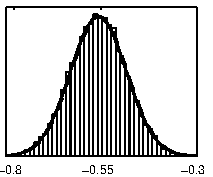
\includegraphics[width=4cm]{hist1}
    }
    ~
    \subfigure[Classification]{ 
      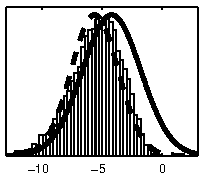
\includegraphics[width=4cm]{hist2}
    }
  \end{center}\caption{Illustration of the Laplace approximation
    (solid line), EP (dashed line) and MCMC (histogram) for the
    conditional posterior of a latent variable
    $p(f_i|\mathcal{D},\theta)$ in two applications. On the left, a
    disease mapping problem with Poisson likelihood \citep[used
    in][]{Vanhatalo+Pietilainen+Vehtari:2010} where the Gaussian
    approximation works well. On the right, a classification problem
    with probit likelihood \citep[used in][]{Vanhatalo+Vehtari:2010}
    where the posterior is skewed and the Gaussian approximation is
    not so good.}
  \label{latent_intergation} 
\end{figure}

\section{Marginal likelihood given parameters}\label{sec_marginal_likelihood}

The marginal likelihood given the parameters,
$p(\mathcal{D}|\theta,\phi) = \int
p(\mb{y}|\f,\phi)p(\f|\mb{X},\theta) d\f$, is an important quantity
when inferring the parameters as discussed in the next section. With a
Gaussian likelihood it has an analytic solution
\eqref{eq_marginal_likelihood_gaussian_case} which gives the log
marginal likelihood
%
\begin{equation}\label{eq_log_marginal_likelihood}
\log p(\mathcal{D}|\theta,\sigma) =  -\frac{n}{2}\log(2\pi) -\frac{1}{2}
\log |\Kff + \sigma^2\mb{I}| -\frac{1}{2} \y^{\text{T}} (\Kff +
\sigma^2\mb{I})^{-1} \y. 
\end{equation}

If the likelihood is not Gaussian, the marginal likelihood needs to be
approximated. The Laplace approximation to the marginal likelihood is
constructed, for example, by making a second order Taylor expansion
for the integrand $p(\mb{y}|\f,\phi)p(\f|\mb{X},\theta)$ around
$\hat{\f}$. This gives a Gaussian integral over $\f$ multiplied by a
constant, and results in the log marginal likelihood approximation
%
\begin{equation}\label{eq_Laplace_marginal_likelihood}
\log p(\mathcal{D}|\theta,\phi) \approx \log
q(\mathcal{D}|\theta,\phi) \propto
-\frac{1}{2}\hat{\f}^{\text{T}}\iKff\hat{\f} + \log p(\mb{y}|\hat{\f},\phi)
- \frac{1}{2} \log |\mb{B}|,  
\end{equation}
%
where $|\mb{B}| = |I+\mb{W}^{1/2}\Kff \mb{W}^{1/2}|$. See also
\citep[][]{Tierney+Kadane:1986,Rue+Martino+Chopin:2009,Vanhatalo+Jylanki+Vehtari:2009}
for more discussion.

EP's marginal likelihood approximation is the normalization constant
%
\begin{equation}
Z_{\text{EP}} = \int p(\f|\mb{X}, \theta)\prod_{i=1}^n \tilde{Z}_i
\N(f_i|\tilde{\mu}_i,\tilde{\sigma}_i^2) d f_i 
\end{equation}
%
in equation \eqref{eq_EP_post}. This is a Gaussian integral multiplied
by a constant $\prod_{i=1}^n \tilde{Z}_i$, giving
%
\begin{align}\label{EP_marg_likelih}
\log p(\mathcal{D}|\theta,\phi) \approx \log Z_{\text{EP}} =&  -\frac{1}{2} \log|K+\tilde{\Sigma}|
-\frac{1}{2}\tilde{\mu}^{\text{T}} \left(K+\tilde{\Sigma}
\right)^{-1}\tilde{\mu} + C_{\text{EP}},
\end{align}
%
where $C_{\text{EP}}$ collects the terms that are not explicit
functions of $\theta$ or $\phi$ (there is an implicit dependence
through the iterative algorithm, though). For more discussion on EP's
marginal likelihood approximation see
\citep{Seeger:2005,Nickisch+Rasmussen:2008}.

\section{Marginalization over parameters}\label{sec_marginalization_over_hyperparam}

The previous section treated methods to evaluate exactly (the Gaussian
case) or approximately (Laplace and EP approximations) the log
marginal likelihood given parameters. Now, we describe approaches for
estimating parameters or integrating numerically over them.

\subsection{Maximum a posterior estimate of parameters}

In a full Bayesian approach we should integrate over all unknowns.
Given we have integrated over the latent variables, it often happens
that the posterior of the parameters is peaked or predictions are
unsensitive to small changes in parameter values.  In such case, we can
approximate the integral over $p(\theta,\phi|\mathcal{D})$ with the
maximum a posterior (MAP) estimate
%
\begin{equation}
\{\hat{\theta}, \hat{\phi}\} = \argmax_{\theta,\phi}
p(\theta,\phi|\mathcal{D}) = \argmin_{\theta,\phi}
\left[ -\log p(\mathcal{D}|\theta,\phi) - \log p(\theta,\phi) \right].
\end{equation}
%
In this approximation, the parameter values are given a point mass one
at the posterior mode, and the marginal of the latent function is
approximated as $p(\f|\mathcal{D}) \approx p(\f|\mathcal{D},
\hat{\theta}, \hat{\phi})$.
%Other way to interpret the parameter optimization is model
%selection over a model family indexed by continuous parameters
%$\theta$ and $\phi$ \citep{Rasmussen+Williams:2006}.
%The negative log posterior cost function $-\log
%p(\mathcal{D}|\theta,\phi) - \log p(\theta,\phi)$ will also be
%called \emph{energy} in the text following the common practice in
%Markov chain Monte Carlo literature.

The log marginal likelihood, and its approximations, are
differentiable with respect to the parameters
\citep{Seeger:2005,Rasmussen+Williams:2006}. Thus, also the log
posterior is differentiable, which allows gradient based optimization.
The advantage of MAP estimate is that it is relatively easy and fast
to evaluate. According to our experience good optimization algorithms
need usually at maximum tens of optimization steps to find the
mode. However, it underestimates the uncertainty in parameters.

\subsection{Grid integration}\label{sec_grid_integration}

Grid integration is based on weighted sum of points evaluated on
grid
%
\begin{equation}\label{eq_grid_integration}
p(\f|\mathcal{D}) \approx \sum_{i=1}^M p(\f|\mathcal{D}, \vartheta_i)
p(\vartheta_i|\mathcal{D}) \Delta_i.
\end{equation}
%
Here $\vartheta = [\theta^{\text{T}}, \phi^{\text{T}}]^{\text{T}}$ and
$\Delta_i$ denotes the area weight appointed to an evaluation point
$\vartheta_i$. The implementation follows INLA
\citep{Rue+Martino+Chopin:2009} and is discussed in detail by
\citet{Vanhatalo+Pietilainen+Vehtari:2010}. The basic idea is to first
locate the posterior mode and then to explore the log posterior
surface so that the bulk of the posterior mass is included in the
integration (see Figure \ref{grid_based_integration}).
The grid search is feasible only for a small number of parameters
since the number of grid points grows exponentially with the dimension
of the parameter space $d$. 

\subsection{Monte Carlo integration}

Monte Carlo integration scales better than the grid integration in
large parameter spaces since its error decreases with a rate that is
independent of the dimension \citep{Robert+Casella:2004}.  There are
two options to find a Monte Carlo estimate for the marginal posterior
$p(\f|\mathcal{D})$. The first option is to sample only the parameters
from their marginal posterior $p(\vartheta|\mathcal{D})$ or from its
approximation (see Figure \ref{is_integration}). In this case, the
posterior marginal of the latent variable is approximated with mixture
distribution as in the grid integration. The alternative is to sample
both the parameters and the latent variables.

The full MCMC is performed by alternate sampling from the conditional
posteriors $p(\f|\mathcal{D},\vartheta)$ and
$p(\vartheta|\mathcal{D},\f)$. Possible choices to sample from the
conditional posterior of the parameters are, e.g., HMC and slice
sampling (SLS) \citep{Neal:2003}. Sampling both the parameters and
latent variables is usually slow since due to the strong correlation
between them
\citep{Vanhatalo+Vehtari:2007,Vanhatalo+Pietilainen+Vehtari:2010}.
Sampling from the (approximate) marginal, $p(\vartheta|\mathcal{D})$,
is an easier task since the parameter space is smaller.

The parameters can be sampled from their marginal posterior (or its
approximation) with HMC, SLS \citep{Neal:2003} or via importance
sampling \citep{Geweke:1989}. In importance sampling, we use a
Gaussian or Student-$t$ proposal distribution $g(\vartheta)$ with mean
$\hat{\vartheta}$ and covariance approximated with the negative
Hessian of the log posterior, and approximate the integral with
%
\begin{equation}
p(\f|\mathcal{D}) \approx \frac{1}{\sum_{i=1}^M w_i} \sum_{i=1}^M
q(\f|\mathcal{D}, \vartheta_i) w_i, 
\end{equation}
%
where $w_i = q(\vartheta^{(i)})/g(\vartheta^{(i)})$ are the importance
weights. In some situations the naive Gaussian or Student-$t$ proposal
distribution is not adequate since the posterior distribution
$q(\vartheta|\mathcal{D})$ may be non-symmetric or the covariance
estimate is poor. An alternative for these situations is the scaled
Student-$t$ proposal distribution \citep{Geweke:1989} which is
adjusted along each main direction of the approximate covariance. The
implementation of the importance sampling is discussed in detail by
\citet{Vanhatalo+Pietilainen+Vehtari:2010}.

The problem with MCMC is that we are not able to draw independent
samples from the posterior. Even with a careful tuning of Markov chain
samplers the autocorrelation is usually so large that the required
sample size is in thousands, which is a clear disadvantage compared
with, for example, the MAP estimate.

\subsection{Central composite design}\label{sec_CCD_integration}

\citet{Rue+Martino+Chopin:2009} suggest a central composite design
(CCD) for choosing the representative points from the posterior of the
parameters when the dimensionality of the parameters, $d$, is moderate
or high. In this setting, the integration is considered as a quadratic
design problem in a $d$ dimensional space with the aim at finding
points that allow to estimate the curvature of the posterior
distribution around the mode. The design used in \pkg{GPstuff} is the
fractional factorial design \citep{Sanchez+Sanchez:2005} augmented
with a center point and a group of $2d$ star points.  The design
points are all on the surface of a $d$-dimensional sphere and the star
points consist of $2d$ points along each axis, which is illustrated in
Figure \ref{ccd_integration}.  The integration is then a finite sum
\eqref{eq_grid_integration} with special weights
\citep{Vanhatalo+Pietilainen+Vehtari:2010}.

CCD integration speeds up the computations considerably compared to
the grid search or Monte Carlo integration since the number of the
design points grows very moderately. The accuracy of the CCD is
between the MAP estimate and the full integration with the grid
search or Monte Carlo. \citet{Rue+Martino+Chopin:2009} report good
results with this integration scheme, and it has worked well in
moderate dimensions in our experiments as well. 
%CCD tries to incorporate the posterior variance of the parameters
%in the inference.
Since CCD is based on the assumption that the posterior of the
parameter is (close to) Gaussian, the densities
$p(\vartheta_i|\mathcal{D})$ at the points on the circumference should
be monitored in order to detect serious discrepancies from this
assumption. These densities are identical if the posterior is Gaussian
and we have located the mode correctly, and thereby great variability
on their values indicates that CCD has failed. The posterior of the
parameters may be far from a Gaussian distribution but for a suitable
transformation, which is made automatically in the toolbox, the
approximation may work well.

\begin{figure}
  \begin{center}
    \subfigure[Grid based ]{
      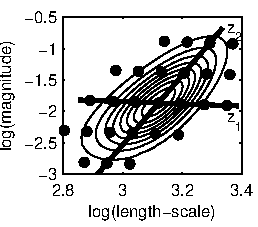
\includegraphics[width=4cm]{grid_based_integration}\label{grid_based_integration}
    }
    ~
    \subfigure[Monte Carlo ]{      
      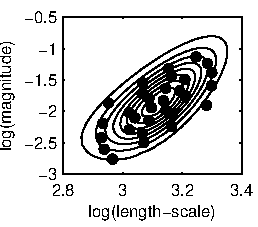
\includegraphics[width=4cm]{is_integration}\label{is_integration}
    }
    \subfigure[Central composite design]{      
      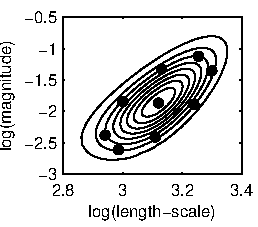
\includegraphics[width=4cm]{ccd_integration}\label{ccd_integration}
    }
  \end{center}\caption{The grid based, Monte Carlo and central
    composite design integration. Contours show the posterior density
    $q(\log(\vartheta)|\mathcal{D})$ and the integration points are
    marked with dots. The left figure shows also the vectors $\mb{z}$
    along which the points are searched in the grid integration and
    central composite design. The integration is conducted over
    $q(\log(\vartheta)|\mathcal{D})$ rather than
    $q(\vartheta|\mathcal{D})$ since the former is closer to Gaussian.
    Reproduced from \citep{Vanhatalo+Pietilainen+Vehtari:2010}.}
  \label{hyperparameter_intergation}
\end{figure}


\section[Getting started with GPstuff: regression and classification]{Getting started with \pkg{GPstuff}: regression and classification}\label{chap:intro_to_GPstuff}

%foo

% In this section, we will discuss the use of \pkg{GPstuff} with two
% classical examples, regression and classification. The section serves
% as a general introduction to the toolbox and discusses many of the
% functionalities of the package that will be present in more advanced
% models as well.

%foo

\subsection{Gaussian process regression}\label{sec:demo_regression1}

The demonstration program \code{demo\_regression1} considers a simple
regression problem $y_i = f(\x_i) + \epsilon_i$, where $\epsilon_i
\sim N(0,\sigma^2)$.  We will show how to construct the model with a
squared exponential covariance function and how to conduct the
inference.

\subsubsection{Constructing the model}

The model construction requires three steps: 1) Create structures that
define likelihood and covariance function, 2) define priors for the
parameters, and 3) create a GP structure where all the above are
stored. These steps are done as follows:
%
\begin{verbatim}
lik = lik_gaussian('sigma2', 0.2^2);
gpcf = gpcf_sexp('lengthScale', [1.1 1.2], 'magnSigma2', 0.2^2)

pn=prior_logunif();
lik = lik_gaussian(lik, 'sigma2_prior', pn);

pl = prior_unif();
pm = prior_sqrtunif();
gpcf = gpcf_sexp(gpcf, 'lengthScale_prior', pl, 'magnSigma2_prior', pm);

gp = gp_set('lik', lik, 'cf', gpcf);
\end{verbatim}
%
Here \code{lik\_gaussian} initializes Gaussian likelihood function and
its parameter values and \code{gpcf\_sexp} initializes the squared
exponential covariance function and its parameter values.
\code{lik\_gaussian} returns structure \code{lik} and
\code{gpcf\_sexp} returns \code{gpcf} that contain all the information
needed in the evaluations (function handles, parameter values etc.).
The next five lines create the prior structures for the parameters of
the observation model and the covariance function, which are set in the
likelihood and covariance function structures. 
%
The last line creates the GP structure by giving it the likelihood
and covariance function.

Using the constructed GP structure, we can evaluate basic summaries
such as covariance matrices, make predictions with the present
parameter values etc. For example, the covariance matrices $\Kff$
and $\mb{C} = \Kff+\sigma^2\mb{I}$ for three two-dimensional
input vectors are:
%
\begin{verbatim}
example_x = [-1 -1 ; 0 0 ; 1 1];
[K, C] = gp_trcov(gp, example_x)
K =
    0.0400    0.0187    0.0019
    0.0187    0.0400    0.0187
    0.0019    0.0187    0.0400
C =
    0.0800    0.0187    0.0019
    0.0187    0.0800    0.0187
    0.0019    0.0187    0.0800
\end{verbatim} 

\subsubsection{MAP estimate for the parameters}

\code{gp\_optim} works as a wrapper for usual gradient based
optimization functions. It is used as follows:
%
\begin{verbatim}
opt=optimset('TolFun',1e-3,'TolX',1e-3,'Display','iter');
gp=gp_optim(gp,x,y,'opt',opt);
\end{verbatim}
\code{gp\_optim} takes a GP structure, training input $\x$,
training target $\y$ (which are defined in
\code{demo\_regression1}) and options, and returns a GP structure
with parameter values optimized to their MAP estimate. By default
\code{gp\_optim} uses \code{fminscg} function, but \code{gp\_optim}
can use also, for example, \code{fminlbfgs} or \code{fminunc}.
Optimization options are set with \code{optimset} function. It is
also possible to set optimisation options as
\begin{verbatim}
opt=struct('TolFun',1e-3,'TolX',1e-3,'Display','iter');
\end{verbatim}
which is useful when using an optimiser not supported by \code{optimset}.
%
All the estimated parameter values can be easily checked using the
function \code{gp\_pak}, which packs all the parameter values from
all the covariance function structures in a vector, usually using
log-transformation (other transformations are also possible). The
second output argument of \code{gp\_pak} lists the labels for the
parameters:
%
\begin{verbatim}
[w,s] = gp_pak(gp);
disp(s), disp(exp(w))

    'log(sexp.magnSigma2)'
    'log(sexp.lengthScale x 2)'
    'log(gaussian.sigma2)'

    2.5981    0.8331    0.7878    0.0427
\end{verbatim}
% 
It is also possible to set the parameter vector of the model to
desired values using \code{gp\_unpak}. \code{gp\_pak} and
\code{gp\_unpak} are used internally to allow use of generic
optimisation and sampling functions, which take the parameter
vector as an input argument.

Predictions for new locations $\tilde{\x}$, given the training data
$(\x,\y)$, are done by \code{gp\_pred} function, which returns the
posterior predictive mean and variance for each $f(\tilde{\x})$ (see
equation \eqref{eq_posterior_predictive_in_gaussian_case}). This is
illustrated below where we create a regular grid where the posterior
mean and variance are computed. The posterior mean $m_{p}(\tilde{\x})$
and the training data points are shown in
Figure~\ref{demo_regression1_fig1}.

\begin{verbatim}
[xt1,xt2]=meshgrid(-1.8:0.1:1.8,-1.8:0.1:1.8);
xt=[xt1(:) xt2(:)];
[Eft_map, Varft_map] = gp_pred(gp, x, y, xt);
\end{verbatim}


\begin{figure}[]
    \begin{center}
      \subfigure[The predictive mean and training data.]{
        \label{}
        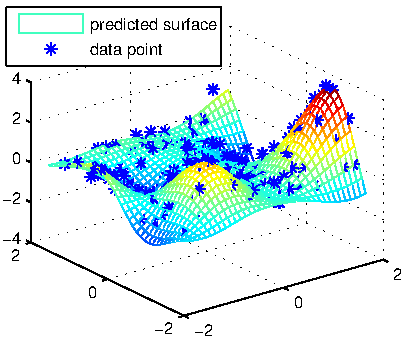
\includegraphics[width=6cm]{demo_regression1_fig1}
      }
      ~
      \subfigure[The marginal posterior predictive distributions
      $p(f_i|\mathcal{D})$. ]{ 
        \label{}
        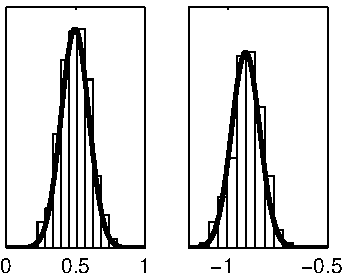
\includegraphics[width=5cm]{demo_regression1_fig3}
       }
       \caption[]{The predictive mean surface, training data, and the
         marginal posterior for two latent variables in
         \code{demo\_regression1}. Histograms show the MCMC solution
         and the grid integration solution is drawn with a
         line.}\label{demo_regression1_fig1}
    \end{center}
\end{figure}

\subsubsection{Marginalization over parameters with grid integration}

To integrate over the parameters we can use any method
described in the section \ref{sec_marginalization_over_hyperparam}.
The grid integration is performed with the following line:
%
\begin{verbatim}
[gp_array, P_TH, th, Eft_ia, Varft_ia, fx_ia, x_ia] = ...
                              gp_ia(gp, x, y, xt, 'int_method', 'grid');
\end{verbatim}
%
\code{gp\_ia} returns an array of GPs (\code{gp\_array}) for parameter
values \code{th} ($[\vartheta_i]_{i=1}^M$) with weights \code{P\_TH}
($[p(\vartheta_i|\mathcal{D}) \Delta_i]_{i=1}^M)$. Since we use the
grid method the weights are proportional to the marginal posterior and
$\Delta_i \equiv 1 \forall i$ (see section
\ref{sec_grid_integration}).  \code{Ef\_ia} and \code{Varf\_ia}
contain the predictive mean and variance at the prediction locations.
The last two output arguments can be used to plot the predictive
distribution $p(\tilde{f}_i|\mathcal{D})$ as demonstrated in Figure
\ref{demo_regression1_fig1}.  \code{x\_ia(i,:)} contains a regular
grid of values $\tilde{f}_i$ and \code{fx\_ia(i,:)} contains
$p(\tilde{f}_i|\mathcal{D})$ at those values.


\subsubsection{Marginalization over parameters with MCMC}

The main function for conducting Markov chain sampling is \code{gp\_mc},
which loops through all the specified samplers in turn and saves the
sampled parameters in a record structure. In later sections, we will
discuss models where also latent variables are sampled, but now we
concentrate on the covariance function parameters, which are sampled
as follows:
%
\begin{verbatim}
[gp_rec,g,opt] = gp_mc(gp, x, y, 'nsamples', 220);
gp_rec = thin(gp_rec, 21, 2);
[Eft_s, Varft_s] = gpmc_preds(rfull, x, y, xt);
[Eft_mc, Varft_mc] = gp_pred(gp_rec, x, y, xt);
\end{verbatim}
% 
The \code{gp\_mc} function generates \code{nsamples} (here 220) Markov
chain samples. At each iteration \code{gp\_mc} runs the actual
samplers.  The function \code{thin} removes the burn-in from the
sample chain (here 21) and thins the chain more (here by 2). This way
we can decrease the autocorrelation between the remaining samples.
\pkg{GPstuff} provides also diagnostic tools for Markov chains. See,
for example,
\citep{Gelman+etal+BDA3:2013,Robert+Casella:2004} for
discussion on convergence and other Markov chain diagnostics. The
function \code{gpmc\_preds} returns the conditional predictive mean
and variance for each sampled parameter value. These are
$\E_{p(\mb{f}|\mb{X}, \mathcal{D}, \mb{\vartheta}^{(s)})}[\tilde{\f}],
s=1,...,M$ and $\VAR_{p(\mb{f}|\mb{X}, \mathcal{D},
  \mb{\vartheta}^{(s)})}[\tilde{\f}], s=1,...,M$, where $M$ is the
number of samples.
%
Marginal predictive mean and variance are computed directly with
\code{gp\_pred}.
%
%We could also use the HMC sampler alone by calling \code{hmc2} but
%then we would get only a matrix of parameter values. The reason
%we use the \code{gp\_mc} is that it stores all the samples in a
%structure that can be passed to \code{thin}, \code{gpmc\_preds} and
%\code{gp\_pred} functions.

\subsection{Gaussian process classification}\label{GP_classification}

%foo

We will now consider a binary GP classification (see
\code{demo\_classific}) with observations, $y_i \in \{-1,1\},
i=1,...,n$, associated with inputs $\mb{X} = \{ \mb{x} \}_ {i=1}^n$.
The observations are considered to be drawn from a Bernoulli
distribution with a success probability $p(y_i=1|\mb{x}_i)$. The
probability is related to the latent function via a sigmoid function
that transforms it to a unit interval. \pkg{GPstuff} provides a probit
and logit transformation, which give
%
\begin{align}\label{eq_probit_likelihood}
p_{\text{probit}}(y_i|f(\x_i)) &= \Phi(y_if(\mb{x}_i)) =
\int_{-\infty}^{y_if(\mb{x}_i)} N(z|0,1) d z \\
p_{\text{logit}}(y_i|f(\x_i)) &= \frac{1}{1 + \exp(-y_if(\x_i))}.\label{eq_logit_likelihood}
\end{align}
% 
Since the likelihood is not Gaussian we need to use approximate
inference methods, discussed in the section
\ref{sec_cond_post_of_latent}.

\subsubsection{Constructing the model}

The model construction for the classification follows closely the
steps presented in the previous section. The model is constructed
as follows:
%
\begin{verbatim}
lik = lik_probit();
gpcf = gpcf_sexp('lengthScale', [0.9 0.9], 'magnSigma2', 10);
gp = gp_set('lik', lik, 'cf', gpcf, 'jitterSigma2', 1e-9);
\end{verbatim}
%
The above lines first initialize the likelihood function, the
covariance function and the GP structure. Since we do not specify
parameter priors, the default priors are used. The model construction
and the inference with logit likelihood (\code{lik\_logit}) would be
similar with probit likelihood. A small jitter value is added to the
diagonal of the training covariance to make certain matrix operations
more stable (this is not usually necessary but is shown here for
illustration).

\subsubsection{Inference with Laplace approximation}\label{sec_classific_Laplace}

The MAP estimate for the parameters can be found using
\code{gp\_optim} as
%
\begin{verbatim}
gp = gp_set(gp, 'latent_method', 'Laplace');
gp = gp_optim(gp,x,y,'opt',opt);
\end{verbatim}
% 
The first line defines which inference method is used for the latent
variables. It initializes the Laplace algorithm and sets needed fields
in the GP structure. The default method for latent variables is
Laplace, so this line could be omitted.
%
\code{gp\_optim} uses the default optimization function,
\code{fminscg}, with the same options as above in the regression
example.

\code{gp\_pred} provides the mean and variance for the latent
variables (first two outputs), the log predictive probability for a
test observation (third output), and mean and variance for the
observations (fourth and fifth output) at test locations \code{xt}.
%
\begin{verbatim}
[Eft_la, Varft_la, lpyt_la, Eyt_la, Varyt_la] = ... 
                           gp_pred(gp, x, y, xt, 'yt', ones(size(xt,1),1) );
\end{verbatim}
%
The first four input arguments are the same as in the section
\ref{sec:demo_regression1}. The fifth and sixth arguments are a
parameter-value pair where \code{yt} tells that we give test
observations \code{ones(size(xt,1),1)} related to \code{xt} as an
optional input, in which case \code{gp\_pred} evaluates their marginal
posterior log predictive probabilities \code{lpyt\_la}. Here we evaluate
the probability to observe class $1$ and thus we give a vector of ones
as test observations. % The probability densities for test observations
% are returned in the fifth output argument
% \code{pyt}. The training data together with predicted
% class probability contours is visualized in Figure
% \ref{demo_classific1_fig1a}.

% \begin{figure}[]
%   \hspace{-3cm}
%     \begin{center}
%       \subfigure[Laplace approximation.]{
%         \label{demo_classific1_fig1a}
%         \includegraphics[width=4cm]{demo_classific1_figLA}
%       }
%       ~
%       \subfigure[Expectation propagation.]{ 
%         \label{demo_classific1_fig1b}
%         \includegraphics[width=4cm]{demo_classific1_figEP}
%        }
%        ~
%        \subfigure[Markov chain Monte Carlo.]{ 
%          \label{demo_classific1_fig1c}
%          \includegraphics[width=4cm]{demo_classific1_figMCMC}
%        }
%        \caption[]{The class probability contours for Laplace
%          approximation, EP, and MCMC solution. The strongest line
%          in the middle is the 50\% probability (the decision
%          boundary) and the thinner lines are 2.5\%, 25\%, 75\% and
%          97.5\% probability contours. It is seen that the decision
%          boundary is approximated similarly with all the methods
%          but there is a larger difference
%          elsewhere.}\label{demo_classific1_fig1}
%     \end{center}
% \end{figure}

\subsubsection{Inference with expectation propagation}

EP works as the Laplace approximation. We only need to set the latent
method to \code{'EP'} but otherwise the commands are the same as above:
%
\begin{verbatim}
gp = gp_set(gp, 'latent_method', 'EP');
gp = gp_optim(gp,x,y,'opt',opt);
[Eft_ep, Varft_ep, lpyt_ep, Eyt_ep, Varyt_ep] = ...
                    gp_pred(gp, x, y, xt, 'yt', ones(size(xt,1),1) );
\end{verbatim}
%
%The EP algorithm is implemented using the nested functions in a
%similar manner as Laplace approximation, for which reason the
%algorithm has to be initialized first. 
% The EP solution for the predicted class probabilities is visualized
% in Figure \ref{demo_classific1_fig1b}.

\subsubsection{Inference with MCMC}

%foo
With MCMC we sample both the latent variables and the parameters:
\begin{verbatim}
gp = gp_set(gp, 'latent_method', 'MCMC', 'jitterSigma2', 1e-6);
[gp_rec,g,opt]=gp_mc(gp, x, y, 'nsamples', 220);
gp_rec=thin(gp_rec,21,2);
[Ef_mc, Varf_mc, lpy_mc, Ey_mc, Vary_mc] = ...
    gp_pred(gp_rec, x, y, xt, 'yt', ones(size(xt,1),1) );
\end{verbatim}
%
For MCMC we need to add a larger jitter on the diagonal to prevent
numerical problems.
%
By default sampling from the latent value distribution $p(\f|\theta,
\mathcal{D})$ is done with the elliptical slice sampling
\citep{Murray+Adams+MacKay:2010}. Other samplers provided by the
\pkg{GPstuff} are a scaled Metropolis Hastings algorithm
\citep{Neal:1998} and a scaled HMC \code{scaled\_hmc}
\citep{Vanhatalo+Vehtari:2007}. From the user point of view, the
actual sampling and prediction are performed similarly as with the
Gaussian likelihood.  The \code{gp\_mc} function handles the sampling
so that it first samples the latent variables from
$p(\f|\theta,\mathcal{D})$ after which it samples the parameters from
$p(\theta|\f,\mathcal{D})$.  This is repeated until \code{nsamples}
samples are drawn.


In classification model MCMC is the most accurate inference method,
then comes EP and Laplace approximation is the worst.  However, the
inference times line up in the opposite order.  The difference between
the approximations is not always this large.  For example, with
Poisson likelihood, discussed in the section \ref{sec_spatial_demo1},
Laplace and EP approximations work, in our experience, practically as
well as MCMC.

\subsubsection{Marginal posterior corrections}

\pkg{GPstuff} also provides methods for marginal posterior corrections using either Laplace or EP as a latent method \citep{Cseke+Heskes:2011}. Provided correction methods are either \texttt{cm2} or \texttt{fact} for Laplace and \texttt{fact} for EP. 

Univariate marginal posterior corrections can be computed with function \texttt{gp\_predcm} which returns the corrected marginal posterior distributtion for the given indices of input/outputs:
\begin{verbatim}
  [pc, fvec, p] = gp_predcm(gp,x,y,'ind', 1, 'fcorr', 'fact');
\end{verbatim}
The returned value \texttt{pc} corresponds to corrected marginal posterior for the latent value $f_1$, \texttt{fvec} corresponds to vector of grid points where \texttt{pc} is evaluated and \texttt{p} is the original Gaussian posterior distribution evaluated at \texttt{fvec}. Marginal posterior corrections can also be used for predictions in \texttt{gp\_pred} and sampling of latent values in \texttt{gp\_rnd} (see \texttt{demo\_improvedmarginals1} and \texttt{demo\_improvedmarginals2}). \texttt{gp\_rnd} uses univariate marginal corrections with Gaussian copula to sample from the joint marginal posterior of several latent values.

\section{Other single latent models}

% In this section, we discuss other example applications where
% \pkg{GPstuff} has been used. 

In this section, we desribe other likelihood functions, which
factorize so that each factor depend only on single latent value.
 
\subsection{Robust regression with Student-$t$ observation model}

A commonly used observation model in the GP regression is the Gaussian
distribution. This is convenient since the marginal likelihood is
analytically tractable. However, a known limitation with the Gaussian
observation model is its non-robustness, due which outlying
observations may significantly reduce the accuracy of the inference
(see Figure~\ref{single_obs_figure}).  A well-known robust observation
model is the Student-$t$ distribution \citep{OHagan:1979}
%
\begin{equation}
 \y | \f, \nu, \sigma_t  \sim \prod_{i=1}^n \frac{\Gamma((\nu+1)/2)}{\Gamma(\nu/2)\sqrt{\nu\pi}\sigma_t}\left(1 +
  \frac{(y_i-f_i)^2}{\nu\sigma_t^2} \right)^{-(\nu+1)/2},
\end{equation}
%
where $\nu$ is the degrees of freedom and $\sigma_t$ the scale
parameter.  The Student-$t$ distribution can be utilized as such or it
can be written via the scale mixture representation
%
\begin{align}
y_i | f_i,\alpha, U_i & \sim N(f_i, \alpha U_i) \label{eq_scale_mixture_1}\\
U_i & \sim \text{Inv-}\chi^2(\nu, \tau^2), \label{eq_scale_mixture_2}
\end{align}
%
where each observation has its own noise variance $\alpha U_i$ that is
$\text{Inv-}\chi^2$ distributed
\citep{Neal:1997,Gelman+etal+BDA3:2013}. The degrees of freedom $\nu$
corresponds to the degrees of freedom in the Student-$t$ distribution
and $\alpha\tau$ corresponds to $\sigma_t$.

\begin{figure}
  \begin{center}
    \subfigure[Gaussian model.]{
      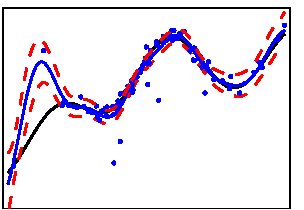
\includegraphics[width=5cm]{neal_data_pic1}\label{neal_data_pic1}
    }    
    ~
    \subfigure[Student-$t$ model.]{ 
      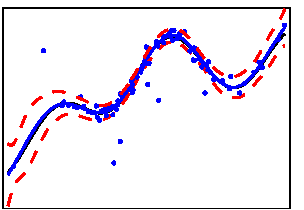
\includegraphics[width=5cm]{neal_data_pic2}\label{neal_data_pic2}
    }
  \end{center}\caption{An example of regression with outliers from
    \citep{Neal:1997}. On the left Gaussian and on the right the
    Student-$t$ model.  The real function is plotted with
    black line.}
  \label{single_obs_figure} 
\end{figure}

In \pkg{GPstuff} both of the representations are implemented. The
scale mixture representation is implemented in
\code{lik\_gaussiansmt} and can be inferred only with MCMC \citep[as
described by][]{Neal:1998}. The Student-$t$ model is
implemented in \code{lik\_t} and can be inferred with Laplace and EP
approximation and MCMC \citep[as described
by][]{Vanhatalo+Jylanki+Vehtari:2009,Jylanki+Vanhatalo+Vehtari:2011}.
These are demonstrated in \code{demo\_regression\_robust}.


\subsection{Count data}\label{sec_spatial_demo1}

Count data are observed in applications. One such common application
is spatial epidemiology, which concerns both describing and
understanding the spatial variation in the disease risk in
geographically referenced health data. One of the most common tasks in
spatial epidemiology is disease mapping, where the aim is to describe
the overall disease distribution on a map and, for example, highlight
areas of elevated or lowered mortality or morbidity risk
\citep[e.g.][]{Lawson:2001,Richardson:2003,Elliot+Wakefield+Best+Briggs:2001}.
Here we build a disease mapping model following the general approach
discussed, for example, by \citet{Best+Richardson+Thomson:2005}. The
data are aggregated into areas with coordinates $\x_i$. The
mortality/morbidity in an area is modeled with a Poisson, negative
binomial or binomial distribution with mean $e_i\mu_i$, where $e_i$ is
the standardized expected number of cases
\citep[e.g.][]{Ahmad+all:2000}, and $\mu_i$ is the relative risk,
whose logarithm is given a GP prior. The aim is to infer the relative
risk. The implementation of these models in \pkg{GPstuff} is discussed
in \citep{Vanhatalo+Vehtari:2007,Vanhatalo+Pietilainen+Vehtari:2010}.

\subsubsection{Poisson}

The Poisson model is implemented in \code{likelih\_poisson} and
it is
%
\begin{equation}
 \y|\f,\mb{e}  \sim \prod_{i=1}^{n} \Poisson(y_i|\exp(f_i)e_i) \label{Poisson_likelihood}
\end{equation}
%
where the vector $\mb{y}$ collects the numbers of deaths for each
area. Here $\mu=\exp(f)$ and its posterior predictive mean and
variance solved in the demo \code{demo\_spatial1} are shown in
Figure~\ref{demo_spatial1_fig1}.
%  where it is
% constructed with the following lines:
% %
% \begin{verbatim}
% pl = prior_t('s2',10);
% pm = prior_sqrtunif();
% gpcf1 = gpcf_matern32('lengthScale_prior', pl, 'magnSigma2_prior', pm);
% lik = lik_poisson();
% gp = gp_set('type', 'FIC', 'lik', lik, 'cf', gpcf1, 'X_u', Xu, ...
%     'jitterSigma2', 0.001, 'infer_params', 'covariance');
% gp = gp_set(gp, 'latent_method', 'Laplace');
% \end{verbatim}
% %
% FIC sparse approximation is used since the data set is rather large
% and inferring full GP would be too slow. The inducing inputs \code{Xu}
% are set to a regular grid (not shown here) in the two dimensional
% lattice and they will be considered fixed
% (\verb|'infer_params', 'covariance'|). In the previous examples only
% covariance functions have required inputs but now we have also the
% expected number of deaths $\mb{e}$ which has to be given to the
% Poisson likelihood. This is given with the extra parameter-value pair
% \verb|'z', ye|. The model is now constructed and we can optimize the
% parameters and evaluate the posterior predictive mean and
% variance of the latent variables shown in
% Figure~\ref{demo_spatial1_fig1} as 
% %
% \begin{verbatim}
% gp = gp_optim(gp,x,y,'z',ye,'opt',opt);
% [Ef, Varf] = gp_pred(gp, x, y, x, 'z', ye, 'tstind', [1:n]);
% \end{verbatim}
% %
% Here, we predict to the same locations that were used for training. In
% this case, since FIC is a limiting case of PIC where each data point
% forms one block, the prediction functions (such as \code{gp\_pred})
% should be given the test index set similarly to the PIC model (see
% section \ref{FIC_PICsparse_approximations}). The demo contains also MCMC
% implementation for the model but it is not discussed here.


\begin{figure}[]
  \begin{center}
    \subfigure[The posterior mean.]{
      \label{}
      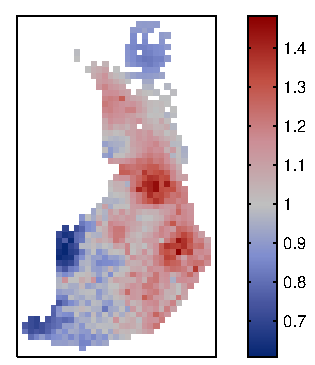
\includegraphics[width=4.2cm]{demo_spatial1_fig1a}
    }
    ~
    \subfigure[The posterior variance.]{ 
      \label{}
      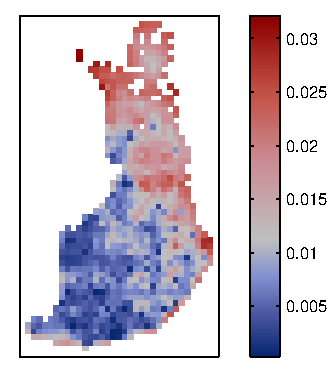
\includegraphics[width=4.4cm]{demo_spatial1_fig1b}
    }
    \caption[]{The posterior predictive mean and variance of the
      relative risk in the \code{demo\_spatial1} data set obtained
      with FIC.}\label{demo_spatial1_fig1}
  \end{center}
\end{figure}

\subsubsection{Negative binomial}\label{sec_spatial_demo2}

The negative binomial distribution is a robust version of the Poisson
distribution similarly as Student-$t$ distribution can be considered
as a robustified Gaussian distribution
\citep{Gelman+etal+BDA3:2013}. In \pkg{GPstuff} it is
parametrized as
%
\begin{equation}
 \y |\f,\mb{e}, r  \sim \prod_{i=1}^n
 \frac{\Gamma(r+y_i)}{y_i!\Gamma(r)}
\left(\frac{r}{r+\mu_i}\right)^r \left(\frac{\mu_i}{r+\mu_i}\right)^{y_i},
\end{equation}
%
where $\mu_i = e_i\exp(f(\x_i))$ and $r$ is the dispersion parameter
governing the variance. The model is demonstrated in
\code{demo\_spatial2}.

\subsubsection{Binomial}

In disease mapping, the Poisson distribution is used to approximate
the true binomial distribution. This approximation works well if the
background population, corresponding to the number of trials in the
binomial distribution, is large. Sometimes this assumption is not
adequate and we need to use the exact binomial observation model
%
\begin{equation}
\y|\f,\mathbf{z} \sim \prod_{i=1}^n \frac{z_i!}{y_i!(z_i-y_i)!} p_i^{y_i}(1-p_i)^{(z_i-y_i)},
\end{equation}
%
where $p_i = \exp(f(\x_i))/ (1+\exp(f(\x_i)))$ is the probability of
success, and the vector $\mathbf{z}$ denotes the number of trials. The
binomial observation model is not limited to spatial modeling but is
an important model for other problems as well. The observation model
is demonstrated in \code{demo\_binomial1} with a one dimensional
simulated data and \code{demo\_binomial\_apc} demonstrates the model in an
incidence risk estimation.

\subsubsection{Hurdle model}
\label{sec_hurdle}

Hurdle models can be used to model excess number of zeros compared
to usual Poisson and negative binomial count models. Hurdle models
assume a two-stage process, where the first process determines
whether the count is larger than zero, and the second process
determines the non-zero count \citep{Mullahy:1986}. These processes
factorize, and thus hurdle model can be implemented using two
independent GPs in GPstuff. \code{lik\_probit} or \code{lik\_logit}
can be used for the zero process and \code{lik\_negbinztr} can be
used for the count part. \code{lik\_negbinztr} provides zero
truncated negative binomial model, which can be used also to
approximate zero-truncated Poisson model by using high dispersion
parameter value. Construction of a hurdle model is demonstrated in
\code{demo\_hurdle}. Gaussian process model with logit negative
binomial hurdle model implemented using \pkg{GPstuff} was used in
reference \citep{Rantonen+etal:2011} to model sick absence days due
to low back symptoms.

Alternative way to model excess number of zeros is to couple the zero
and count processes as in zero-inflated negative binomial model
described in section~\ref{sec_zinegbin}.

%
\subsection{Log-Gaussian Cox process}

Log-Gaussian Cox-process is an inhomogeneous Poisson process model
used for point data, with unknown intensity function $\lambda(\x)$,
modeled with log-Gaussian process so that $f(\x)=\log \lambda(\x)$
\citep[see][]{Rathbun+Cressie:1994,Moller+Syversveen+Waagepetersen:1998}.
%
If the data are points $\mb{X}=\x_i;$ $i=1,2,\ldots,n$ on a finite region
$\mathcal{V}$ in $\Re^d$, then the likelihood of the unknown
function $f$ is
\begin{align}
  p(\mb{X}|f)=\exp\left\{-\left(\int_{\mathcal{V}} \exp(f(\x)) d\x
\right)+\sum_{i=1}^{n} f(\x_i) \right\}.
\end{align}
Evaluation of the likelihood would require nontrivial integration over
the exponential of GP.  \citet{Moller+Syversveen+Waagepetersen:1998}
propose to discretise the region $\mathcal{V}$ and assume locally
constant intensity in subregions. This transforms the problem to a
form equivalent to having Poisson model for each subregion. Likelihood
after the discretisation is
\begin{align}
  p(\mb{X}|f)\approx \prod_{k=1}^K \Poisson(y_k|\exp(f(\dot{\x}_k))),
\end{align}
where $\dot{\x}$ is the coordinate of the $k$th sub-region and $y_k$
is the number of data points in it. \citet{Tokdar+Ghosh:2007} proved
the posterior consistency in limit when sizes of subregions go to
zero.

The log-Gaussian Cox process with Laplace and EP approximation is
implemented in the function \code{lgcp} for one or two dimensional
input data. The usage of the function is demonstrated in
\code{demo\_lgcp}. This demo analyzes two data sets.  The first one is
one dimensional case data with coal mine disasters (from R
distribution). The data contain the dates of 191 coal mine explosions
that killed ten or more men in Britain between 15 March 1851 and 22
March 1962. The analysis is conducted using expectation propagation
and CCD integration over the parameters and the results are shown
in Figure \ref{fig_demo_lgcp}. The second data are the redwood data
(from R distribution). This data contain 195 locations of redwood
trees in two dimensional lattice. The smoothed intensity surface is
shown in Figure \ref{fig_demo_lgcp}.


\begin{figure}[]
  \begin{center}
    \subfigure[Coal mine disasters.]{
      \label{}
      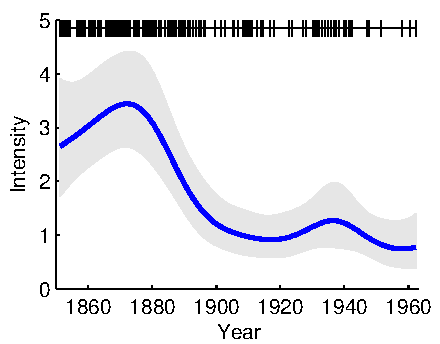
\includegraphics[width=5.5cm]{demo_lgcp_fig1}
    }
    ~
    \subfigure[Redwood data.]{ 
      \label{}
      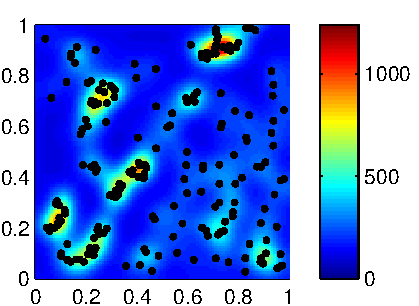
\includegraphics[width=5.5cm]{demo_lgcp_fig2}
    }
    \caption[]{Two intensity surfaces estimated with log-Gaussian Cox
      process. The figures are from the \code{demo\_lgcp}, where the
      aim is to study an underlying intensity surface of a point
      process. On the left a temporal and on the right a spatial point
      process.}\label{fig_demo_lgcp}
  \end{center}
\end{figure}

\subsection{Accelerated failure time survival models}

The accelerated failure time survival models are demonstrated in
\code{demo\_survival\_aft}. These models can be used to model also
other positive continuous data with or without censoring.

\subsubsection{Weibull}
\label{sec_weibull_demo}

The Weibull distribution is a widely used parametric baseline hazard
function in survival analysis \citep{Ibrahim+Chen+Sinha:2001}. The
hazard rate for the observation $i$ is
\begin{equation}
  h_i(y)=h_0(y)\exp(f(\x_i)),
\end{equation}
where $y>0$ and the baseline hazard $h_0(y)$ is assumed to follow the
Weibull distribution parametrized in \pkg{GPstuff} as
\begin{equation}
  h_0(y) = r y^{r-1},
\end{equation}
where $r>0$ is the shape parameter. This follows the parametrization
used in \citet{Martino:2011}. The likelihood defined as
\begin{equation}
  L = \prod_{i=1}^n r^{1-z_i} \exp \left( (1-z_i)f(\x_i)+(1-z_i)(r-1)\log(y_i)-\exp(f(\x_i))y_i^r \right),
\end{equation}
where $\mathbf{z}$ is a vector of censoring indicators with $z_i = 0$ for
uncensored event and $z_i = 1$ for right censored event for
observation $i$. Here we present only the likelihood function because we don't have observation model for the censoring. 

\subsubsection{Log-Gaussian}
With Log-Gaussian survival model the logarithms of survival times are assumed to be normally distributed.

The likelihood is defined as
\begin{eqnarray}
  L = && \prod_{i=1}^n (2\pi \sigma^2)^{-(1-z_i)/2}y_i^{1-z_i} \exp \left(-\frac{1}{2\sigma^2}(1-z_i)(\log (y_i) - f(\x_i))^2\right) \\ \nonumber
  &\times & \left(1 - \Phi \left(\frac{\log(y_i) - f(\x_i)}{\sigma}\right)\right)^{z_i} 
\end{eqnarray}
where $\sigma$ is the scale parameter.

%      p(y|f, z) = || i=1 [ (2*pi*s^2)^(-(1-z_i)/2)*y_i^-(1-z_i)
%                            *exp(-1/(2*s^2)*(1-z_i)*(log(y_i) - f_i)^2)
%                            *(1-norm_cdf((log(y_i)-f_i)/s))^z_i ]
\subsubsection{Log-logistic}

The log-logistic likelihood is defined as

\begin{equation}
  L = \prod_{i=1}^n \left( \frac{ry^{r-1}}{\exp(f(\x_i))} \right)^{1-z_i} \left( 1 + \left(\frac{y}{\exp(f(\x_i))}\right)^r \right)^{z_i-2},
\end{equation}
where $r$ is the shape parameter and $z_i$ the censoring indicators.
%    The likelihood is defined as follows:
%                  __ n
%      p(y|f, z) = || i=1 [ (r/exp(f_i)*(y_i/exp(f_i))^(r-1)/
%                               (1+(y_i/exp(f_i))^r))^(1-z_i)
%                               *(1+(y_i/exp(f_i))^r)^(-z_i) ]
%                           

\subsection{Derivative observations in GP regression}

Incorporating derivative observations in GP regression is fairly
straightforward, because a derivative of Gaussian process is a
Gaussian process. In short, derivative observation are taken into
account by extending covariance matrices to include derivative
observations. This is done by forming joint covariance matrices of
function values and derivatives. Following equations
\citep{Rasmussen+Williams:2006} state how the covariances between
function values and derivatives, and between derivatives are
calculated
% 
\begin{equation}
  \COV(f_i,\frac{\partial f_j}{\partial x_{dj}}) = \frac{\partial k(\textbf{x}_i,\textbf{x}_j}{\partial x_{dj}}), \qquad
  \COV(\frac{\partial f_i}{\partial x_{di}},\frac{\partial f_j}{\partial x_{ej}}) = \frac{\partial^2 k(\textbf{x}_i,\textbf{x}_j}{\partial x_{di}\partial x_{ej}}.\nonumber
\end{equation}
% 
The joint covariance matrix for function values and derivatives is of
the following form
% 
\begin{eqnarray}
  \textbf{K} &=&
  \left[
    \begin{array}{cc}
      \textbf{K}_{ff} & \textbf{K}_{fD}\\
      \textbf{K}_{Df}& \textbf{K}_{DD}
    \end{array}\nonumber
  \right]\\
  \nonumber\\
  \textbf{K}_{ff}^{ij} &=& k(\textbf{x}_i,\textbf{x}_j),\nonumber\\
  \textbf{K}_{Df}^{ij} &=& \frac{\partial k(\textbf{x}_i,\textbf{x}_j)}{\partial x_{di}},\nonumber\\
  \textbf{K}_{fD} &=& (\textbf{K}_{Df})^\top,\label{DerKder3} \nonumber\\
  \textbf{K}_{DD}^{ij} &=& \frac{\partial^2 k(\textbf{x}_i,\textbf{x}_j)}{\partial x_{di} \partial x_{ej}},\nonumber
\end{eqnarray}
% 
Prediction is done as usual but with derivative observations joint
covariance matrices are to be used instead of the normal ones.

Using derivative observations in GPstuff requires two steps: when
initializing the GP structure one must set option
\code{'derivobs'} to \code{'on'}. The second step is to form
right sized observation vector. With input size $n \times m$ the
observation vector with derivatives should be of size $n + m \cdot
n$. The observation vector is constructed by adding partial
derivative observations after function value observations
% 
\begin{equation}
  \textbf{y}_{obs} =
  \left[
    \begin{array}{c}
      y(\textbf{x})\\
      \frac{\partial y(\textbf{x})}{\partial x_1} \\
      \vdots\\
      \frac{\partial y(\textbf{x})}{\partial x_m}
    \end{array}
  \right].
\end{equation}
% 
Different noise level could be assumed for function values and
derivative observations but at the moment the implementation allows
only same noise for all the observations. The use of derivative
observations is demonstrated in \code{demo\_derivativeobs}.

% \subsubsection{GP regression with derivatives: demo\_derivativeobs}

% In this section we will go through the demonstration
% \code{demo\_derivativeobs}.  This demo will present the main
% differences between GP regression with and without derivative
% observations and how to use them with GPstuff. The demo is divided in
% two parts: in the first part the GP regression is done without
% derivatives observations and in the second with them. Here we will
% present the lines of the second part because the first part is almost
% identical with just a few differences.

% First we create the artificial data. Notice how observation vector is
% defined differently for GP models with and without derivatives
% observations. With derivative observations the observation vector
% includes the partial derivative observations which are set as a column
% vector after function value observations

% \begin{verbatim}
% % Create the data
% tp=9;                                  %number of training points -1
% x=-2:5/tp:2;
% y=sin(x).*cos(x).^2;                   % The underlying process f
% dy=cos(x).^3 - 2*sin(x).^2.*cos(x);    % Derivative of the process
% koh=0.06;                              % noise standard deviation

% % Add noise
% y=y + koh*randn(size(y));
% dy=dy + koh*randn(size(dy));           % derivative obs are also noisy
% x=x';           
% dy=dy';

% y=y';          % observation vector without derivative observations
% y2=[y;dy];     % observation vector with derivative observations
% \end{verbatim}

% %  The model constructed for regression is a full GP with a Gaussian
% %  likelihood. The covariance function is squared exponential, which
% %  is the only covariance function that is compatible with derivative
% %  observations at the moment. The field \code{derivobs} is added
% %  into \code{gp\_set(\dots)} so that the inference is done with
% %  derivative observations. Field \code{DerivativeCheck} should also
% %  be added to \code{optimset(\dots)} when taking the predictions so
% %  that derivative observations can be used.

% %  \scriptsize
% %  \begin{verbatim}
% %  gpcf1 = gpcf_sexp('lengthScale', 0.5, 'magnSigma2', .5);
% %  pl = prior_t();                   % a prior structure
% %  pm = prior_sqrtt();               % a prior structure
% %  gpcf1 = gpcf_sexp(gpcf1, 'lengthScale_prior', pl, 'magnSigma2_prior', pm);

% %  gp = gp_set('cf', gpcf1, 'derivobs', 'on');
% %  \end{verbatim}
% %  \normalsize
% %  %
% %  \begin{figure}[!htb]
% %    \centering
% %    \subfigure[Standard GP]{\includegraphics[width=5.3cm]{demo_derivative_fig1}}
% %    \subfigure[GP with der. observations]{\includegraphics[width=5.3cm]{demo_derivative_fig2}}
% %    \caption{GP predictions of the process f with (fig b) and without (fig a) derivative observations.}
% %    \label{demo_derivative_fig}
% %  \end{figure}
% %  %
% %  In the figure \ref{demo_derivative_fig} are the predictions,
% %  observations, the underlying process and the 95\,\% confidence
% %  intervals for both GP model with and GP model without derivative
% %  observations.

Derivative process can be also used to construct a monotonicity constraint as described in section~\ref{sec_monotonic}.

\subsection{Quantile Regression}

Quantile regression is used for estimating quantiles of the response
variable as a function of input variables \citep{Boukouvalas:2012}.

The likelihood is defines as
\begin{align}
p(y | f, \sigma, \tau) = \frac{\tau(1-\tau)}{\sigma}\exp\left[-\frac{y-f}{\sigma}(\tau - I(y \le f))\right],
\end{align}
where $\tau$ is the quantile of interest and $\sigma$ is the standard
deviation. $I(y \le f)$ is 1 if the condition inside brackets is true
and 0 otherwise. Because the logarithm of the likelihood is not twice
differentiable at the mode, Laplace approximation cannot be used for
inference with Quantile Regression. Quantile Regression with EP and
MCMC is demonstrated in \code{demo\_qgp} with toy data.

%    The likelihood is defined as follows:
%                            __ n
%      p(y|f, sigma2, tau) = || i=1 tau*(1-tau)/sigma*exp(-(y-f)/sigma*
%                                 (tau - I(t <= f)))
%    
%    where tau is the quantile of interest, sigma is the standard deviation
%    of the distribution and I(t <= f) = 1 if t <= f, 0 otherwise.
%
%    Note that because the form of the likelihood, second order derivatives
%    with respect to latent values are 0. Because this, EP should be used
%    instead of Laplace approximation.    
%
%  See also
%    GP_SET, PRIOR_*, LIK_*
%
%   References
%     Boukouvalas et al. (2012). Direct Gaussian Process Quantile Regression
%     Using Expectation Propagation. Appearing in Proceedings of the 29th
%     International Conference on Machine Learning, Edinburg, Scotland, UK,
%     2012.


\section{Multilatent models}
\label{sec:multilatent-models}

The multilatent models consist of models where individual likelihood
factors depend on multiple latent variables. In this section we
shortly summarize such models in GPstuff.

\subsection{Multiclass classification}

In multiclass classification problems the target variables have more
than two possible class labels, $y_i\in\{1,\ldots,c\}$, where $c>2$ is
the number of classes. In \pkg{GPstuff}, multi-class classification
can be made either using the softmax likelihood (\code{lik\_softmax})
%
\begin{eqnarray}
p(y_i|\f_i)=\frac{\exp(f_i^{y_i})}{\sum_{j=1}^c\exp(f_i^{j})},
\end{eqnarray}
where $\f_i=\left[f_i^1,\ldots,f_i^c\right]^T$, or the multinomial
probit likelihood  (\code{lik\_multinomialprobit})
\begin{eqnarray}
p(y_i|\f_i)=\mathrm{E}_{p(u_i)} \left\{\prod_{j=1,j\neq y_i}^c \Phi (u_i+f^{y_i}_i-f^j_i)
\right\},
\end{eqnarray}
where the auxiliary variable $u_i$ is distributed as
$p(u_i)=\mathcal{N}(u_i|0,1)$, and $\Phi(x)$ denotes the cumulative
density function of the standard normal distribution.
%
In Gaussian process literature for multiclass classification, a common
assumption is to introduce $c$ independent prior processes that are
associated with $c$ classes \citep[see, e.g.,][]{Rasmussen+Williams:2006}.
%
By assuming zero-mean Gaussian processes for latent functions
associated with different classes, we obtain a zero-mean Gaussian
prior
\begin{eqnarray}
  p(\f|X)=\mathcal{N}(\f|\mathbf{0}, K),
\end{eqnarray}
where
$\f=\left[f_1^1,\ldots,f_n^1,f_1^2,\ldots,f_n^2,\ldots,f_1^c,\ldots,f_n^c\right]^T$
and $K$ is a $cn \times cn$ block-diagonal covariance matrix with
matrices $K^1, K^2,\ldots,K^c$ (each of size $n \times n$) on its
diagonal.

Inference for softmax can be made with MCMC or Laplace approximation.
As described by \citet{Williams+Barber:1998} and
\citet{Rasmussen+Williams:2006}, using the Laplace approximation for
the softmax likelihood with the uncorrelated prior processes, the
posterior computations can be done efficiently in a way that scales
linearly in $c$, which is also implemented in
\pkg{GPstuff}. Multiclass classification with softmax is demonstrated
in \code{demo\_multiclass}.

Inference for multinomial probit can be made with expectation
propagation by using a nested EP approach that does not require
numerical quadratures or sampling for estimation of the tilted moments
and predictive probabilities, as proposed by \citet{Riihimaki+Jylanki+Vehtari:2013}.
%
Similarly to softmax with Laplace's method, the nested EP approach
leads to low-rank site approximations which retain all posterior
couplings but results in linear computational scaling with respect to
$c$.
%
Multiclass classification with the multinomial probit likelihood is
demonstrated in \code{demo\_multiclass\_nested\_ep}.
% In multiclass classification problems the target variables have more
% than two possible class labels, $y_i\in\{1,\ldots,c\}$, where $c>2$ is
% the number of classes. In \pkg{GPstuff}, multi-class classification
% can be made using the softmax likelihood (\code{lik\_softmax})
% %
% \begin{eqnarray}
% p(y_i|\f_i)=\frac{\exp(f_i^{y_i})}{\sum_{j=1}^c\exp(f_i^{j})},
% \end{eqnarray}
% where $\f_i=\left[f_i^1,\ldots,f_i^c\right]^T$.
% %
% In Gaussian process literature for multiclass classification, a common
% assumption is to introduce $c$ independent prior processes that are
% associated with $c$ classes \citep[see, e.g.,][]{Rasmussen+Williams:2006}.
% %
% By assuming zero-mean Gaussian processes for latent functions
% associated with different classes, we obtain a zero-mean Gaussian
% prior
% \begin{eqnarray}
%   p(\f|X)=\mathcal{N}(\f|\mathbf{0}, K),
% \end{eqnarray}
% where
% $\f=\left[f_1^1,\ldots,f_n^1,f_1^2,\ldots,f_n^2,\ldots,f_1^c,\ldots,f_n^c\right]^T$
% and $K$ is a $cn \times cn$ block-diagonal covariance matrix with
% matrices $K^1, K^2,\ldots,K^c$ (each of size $n \times n$) on its
% diagonal.
% %
% Inference for softmax can be made with MCMC or Laplace approximation.
% As described by \citet{Williams+Barber:1998} and
% \citet{Rasmussen+Williams:2006}, using the Laplace approximation for
% the softmax likelihood with the uncorrelated prior processes, the
% posterior computations can be done efficiently in a way that scales
% linearly in $c$, which is also implemented in
% \pkg{GPstuff}. Multiclass classification with softmax is demonstrated
% in \code{demo\_multiclass}.

\subsection{Multinomial}

The multinomial model (\code{lik\_multinomial}) is an extension of the
multiclass classification to situation where each observation consist
of counts of class observations. Let $y_i = [y_{i,1},\ldots,y_{i,c}]$,
where $c>2$, be a vector of counts of class observations related to
inputs $x_i$ so that
%
\begin{equation}
y_i \sim \text{Multinomial}([p_{i,1},\ldots,p_{i,c}],n_i)
\end{equation}
%
where $n_i=\sum_{j=1}^c y_{i,j}$. The propability to observe class $j$ is
%
\begin{eqnarray}
p_{i,j}=\frac{\exp(f_i^j)}{\sum_{j=1}^c\exp(f_i^j)},
\end{eqnarray}
%
where $\f_i=\left[f_i^1,\ldots,f_i^c\right]^T$. As in multiclass
classification we can introduce $c$ independent prior processes that
are associated with $c$ classes.
%
By assuming zero-mean Gaussian processes for latent functions
associated with different classes, we obtain a zero-mean Gaussian
prior
\begin{eqnarray}
  p(\f|X)=\mathcal{N}(\f|\mathbf{0}, K),
\end{eqnarray}
where
$\f=\left[f_1^1,\ldots,f_n^1,f_1^2,\ldots,f_n^2,\ldots,f_1^c,\ldots,f_n^c\right]^T$
and $K$ is a $cn \times cn$ block-diagonal covariance matrix with
matrices $K^1, K^2,\ldots,K^c$ (each of size $n \times n$) on its
diagonal. This model is demonstrated in \code{demo\_multinomial} and
it has been used, for example, in
\citep{Juntunen+Vanhatalo+Peltonen+Mantyniemi:2012}.

\subsection{Cox proportional hazard model}

For the individual $i$, where $i=1,\ldots,n$, we have observed
survival time $y_i$ (possibly right censored) with censoring indicator
$\delta_i$, where $\delta_i=0$ if the $i$th observation is uncensored
and $\delta_i=1$ if the observation is right censored. The traditional
approach to analyze continuous time-to-event data is to assume the Cox
proportional hazard model \citep{Cox:1972}.
\begin{equation}
h_i(t)=h_0(t)\exp(\bm{x}^T_i\bm{\beta}),
\end{equation}
where $h_0$ is the unspecified baseline hazard rate, $\bm{x}_i$ is the
$d\times1$ vector of covariates for the $i$th patient and $\bm{\beta}$
is the vector of regression coefficients. The matrix
$X=[\bm{x}_1,\ldots,\bm{x}_n]^T$ of size $n\times d$ includes all
covariate observations.

The Cox model with linear predictor can be extended to more general
form to enable, for example, additive and non-linear effects of
covariates \citep{Kneib:2006,Martino:2011}. We extend the proportional
hazard model by
\begin{equation}
h_i(t)=\exp(\log(h_0(t))+\eta_i(\bm{x}_i)),
\end{equation}
where the linear predictor is replaced with the latent predictor
$\eta_i$ depending on the covariates $\bm{x}_i$. By assuming a
Gaussian process prior over
$\bm{\eta}=(\eta_1,\ldots,\eta_n)^T$, smooth nonlinear effects of
continuous covariates are possible, and if there are dependencies
between covariates, GP can model these interactions implicitly. 

A piecewise log-constant baseline hazard \citep[see,
e.g.][]{Ibrahim+Chen+Sinha:2001,Martino:2011} is assumed by
partitioning the time axis into $K$ intervals with equal lengths:
$0=s_0<s_1<s_2<\ldots<s_K$, where $s_K>y_i$ for all $i=1,\ldots,n$. In
the interval $k$ (where $k=1,\ldots,K$), hazard is assumed to be
constant:
\begin{eqnarray}
h_0(t)=\lambda_k&\mathrm{for}&t\in(s_{k-1},s_k].
\end{eqnarray}
For the $i$th individual the hazard rate in the $k$th time interval is
then
\begin{eqnarray}
h_i(t)=\exp(f_k+\eta_i(\bm{x}_i)), & t\in(s_{k-1},s_k],
\end{eqnarray}
where $f_k=\log(\lambda_k)$. To assume smooth hazard rate functions,
we place another Gaussian process prior for
$\bm{f}=(f_1,\ldots,f_K)^T$. We define a vector containing the mean
locations of $K$ time intervals as
$\bm{\tau}=(\tau_1,\ldots,\tau_K)^T$. 

% The two latent processes are assumed to a priori
% independent/uncorrelated, and this leads to a prior covariance matrix
% with a block diagonal structure.

The likelihood contribution for the possibly right censored $i$th
observation $(y_i,\delta_i)$ is assumed to be
\begin{equation}
l_i=h_i(y_i)^{(1-\delta_i)} \exp \left(
  -\int_0^{y_i}h_i(t)dt \right).
\end{equation}
Using the piecewise log-constant assumption for the hazard rate
function, the contribution of the observation $i$ for the likelihood
results in
\begin{equation}
l_i=[\lambda_k \exp(\eta_i)]^{(1-\delta_i)}\exp \left( -[(y_i-s_{k-1})\lambda_k
  + \sum_{g=1}^{k-1}(s_g-s_{g-1})\lambda_g ]\exp(\eta_i) \right),
\end{equation}
where $y_i\in(s_{k-1},s_k]$
\citep{Ibrahim+Chen+Sinha:2001,Martino:2011}. By applying the Bayes
theorem, the prior information and likelihood contributions are
combined, and the posterior distribution of the latent variables can
be computed. Due to the form of the likelihood function, the resulting
posterior becomes non-Gaussian and analytically exact inference is
intractable. \pkg{GPstuff} supports MCMC and Laplace approximation to
integrate over the latent variables. The use of Gaussian process Cox
proportional hazard model is demonstrated in
\code{demo\_survival\_coxph}. The Gaussian process Cox proportional
hazard model implemented with GPstuff was used in reference
\citep{Joensuu+etal:2012a} to model risk of gastrointestinal stromal
tumour recurrence after surgery.

%    creates a proportional hazard model where a piecewise log-constant
%    baseline hazard is assumed.  
%    
%    The likelihood contribution for the ith observation is
%
%      l_i = h_i(y_i)^(1-z_i)*[exp(-int_0^y_i*h_i dt)],
%    
%    where hazard is h_i=h_0(y_i)*exp(f_i). A zero mean Gaussian process
%    prior is placed for f = [f_1, f_2,...,f_n] ~ N(0, C). C is the
%    covariance matrix, whose elements are given as C_ij = c(x_i, x_j |
%    th). The function c(x_i, x_j| th) is covariance function and th its
%    parameters, hyperparameters. We place a hyperprior for
%    hyperparameters, p(th). 
%
%    The time axis is partioned into K intervals with equal lengths:
%    0 = s_0 < s_1 < ... < s_K, where s_K > y_i for all i. The baseline
%    hazard rate function h_0 is piecewise constant,  
%
%      h_0(t) = la_k,
%
%    when t belongs to the interval (s_{k-1},s_k] and where ft_k=log(la_k).
%    The hazard rate function is smoothed by assuming another Gaussian
%    process prior ft = [ft_1, ft_2,...,ft_K] ~ N(0, C). 
%
%    z is a vector of censoring indicators with z = 0 for uncensored event
%    and z = 1 for right censored event. 
%
%    When using the Coxph likelihood you need to give the vector z
%    as an extra parameter to each function that requires also y. 
%    For example, you should call gpla_e as follows: gpla_e(w, gp,
%    x, y, 'z', z)

\subsection{Zero-inflated negative binomial}
\label{sec_zinegbin}

Zero-inflated negative binomial model is suitable for modelling count
variables with excessive number of zero observations compared to usual
Poisson and negative binomial count models. Zero-inflated negative
binomial models assume a two-stage process, where the first process
determines whether the count is larger than zero, and the second
process determines the non-zero count \citep{Mullahy:1986}.
In \pkg{GPstuff}, these processes are assumed independent a priori, but they
become a posteriori dependent through the likelihood function
\begin{align}
  p + & (1-p)\mathrm{NegBin}(y|y=0),  \quad\mathrm{when}\quad y=0\\
      & (1-p)\mathrm{NegBin}(y|y>0),  \quad\mathrm{when}\quad y>0,
\end{align}
where the probability p is given by a binary classifier with logit
likelihood. NegBin is the Negative-binomial distribution parametrized
for the $i$'th observation as
\begin{equation}
 \y |\f,\mb{e}, r  \sim \prod_{i=1}^n
 \frac{\Gamma(r+y_i)}{y_i!\Gamma(r)}
\left(\frac{r}{r+\mu_i}\right)^r \left(\frac{\mu_i}{r+\mu_i}\right)^{y_i},
\end{equation}
%
where $\mu_i = e_i\exp(f(\x_i))$ and $r$ is the dispersion parameter
governing the variance. In \pkg{GPstuff}, the latent value vector
$\f=[\f_1^T \f_2^T]^T$ has length $2N$, where $N$ is the number of
observations. The latents $\f_1$ are associated with the
classification process and the latents $\f_2$ with the
negative-binomial count process. %The model is demonstrated in ?.

%    The likelihood is defined as follows:
%     
%      p + (1-p)*NegBin(y|y=0),    when y=0
%          (1-p)*NegBin(y|y>0),    when y>0,
%      where the probability p is given by a binary classifier with Logit
%      likelihood and NegBin is the Negative-binomial distribution
%      parametrized for the i'th observation as
%      NegBin(y_i) =   [ (r/(r+mu_i))^r * gamma(r+y_i)
%                        / ( gamma(r)*gamma(y_i+1) )
%                        * (mu/(r+mu_i))^y_i ]
%
%    where mu_i = z_i*exp(f_i) and r is the dispersion parameter.
%    z is a vector of expected mean and f the latent value vector
%    whose components are transformed to relative risk
%    exp(f_i). 
%
%    The latent value vector f=[f1^T f2^T]^T has length 2*N, where N is the
%    number of observations. The latents f1 are associated with the
%    classification process and the latents f2 with Negative-binomial count
%    process.
%
%    When using the Zinegbin likelihood you need to give the vector z
%    as an extra parameter to each function that requires also y. 
%    For example, you should call gpla_nd_e as follows: gpla_nd_e(w, gp,
%    x, y, 'z', z)

\subsection{Density estimation and regression}

Logistic Gaussian process can be used for flexible density estimation
and density regression. \pkg{GPstuff} includes implementation based on
Laplace (and MCMC) approximation as described in
\citep{Riihimaki+Vehtari:2012}.

The likelihood is defined as
\begin{align}
  p(\x|\f)=\prod_{i=1}^n \frac{\exp(f_i)}{\sum_{j=1}^n \exp(f_j)}.
\end{align}
For the latent function $f$, we assume
the model $f(\x) = g(\x)+\h(\x)^T \bm{\beta}$, where the GP prior
$g(\x)$ is combined with the explicit basis functions $\h(\x)$.
Regression coefficients are denoted with $\bm{\beta}$, and by placing
a Gaussian prior $\bm{\beta}\sim \mathcal{N}(\bb,B)$ with mean $\bb$
and covariance $B$, the parameters $\bm{\beta}$ can be integrated out
from the model, which results in the following GP prior for $f$:
\begin{equation}\label{gp_process}
  f(\x)\sim \mathcal{GP}\left(\h(\x)^T\bb,\kappa(\x,\x')+\h(\x)^TB\h(\x')\right).
\end{equation}
%
For the explicit basis functions, we use the second-order polynomials
%
%$\h(\x)=[x_1 \quad x_1^2 \, \cdots \, x_d \quad x_d^2]^T$,
%
which leads to a GP prior that can favour density estimates where the
tails of the distribution go eventually to zero.

We use finite-dimensional approximation and evaluate the integral and
the Gaussian process in a grid.
%
We approximate inference for logistic Gaussian process density
estimation in a grid using Laplace's method or MCMC to integrate over
the non-Gaussian posterior distribution of latent values \citep[see
details in][]{Riihimaki+Vehtari:2012}.

Logistic Gaussian processes are also suitable for estimating
conditional densities $p(t|\x)$, where $t$ is a response variable. We
discretize both input and target space in a finite region to model the
conditional densities with the logistic GP.
%
To approximate the resulting non-Gaussian posterior distribution, we
use again Laplace's method.

1D and 2D density estimation and density regression are implemented in
the function \code{lgpdens}. The usage of the function is demonstrated
in \code{demo\_lgpdens}.

\begin{figure}[]
  \begin{center}
    \subfigure[Galaxy data.]{
      \label{}
      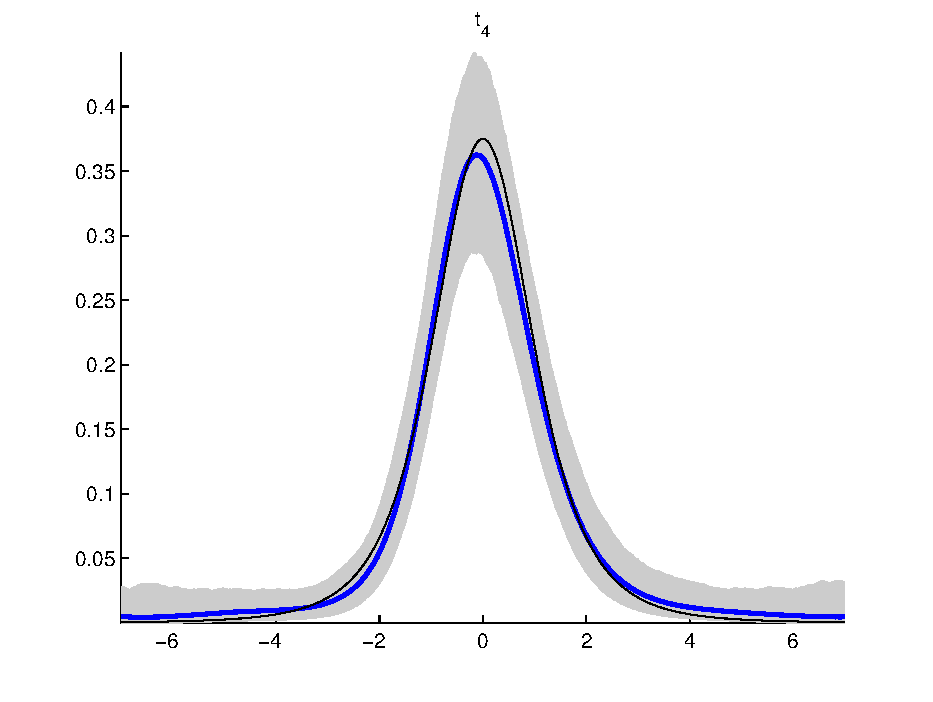
\includegraphics[width=7cm]{demo_lgpdens_fig1}
    }
    ~
    \subfigure[Old faithful data.]{ 
      \label{}
      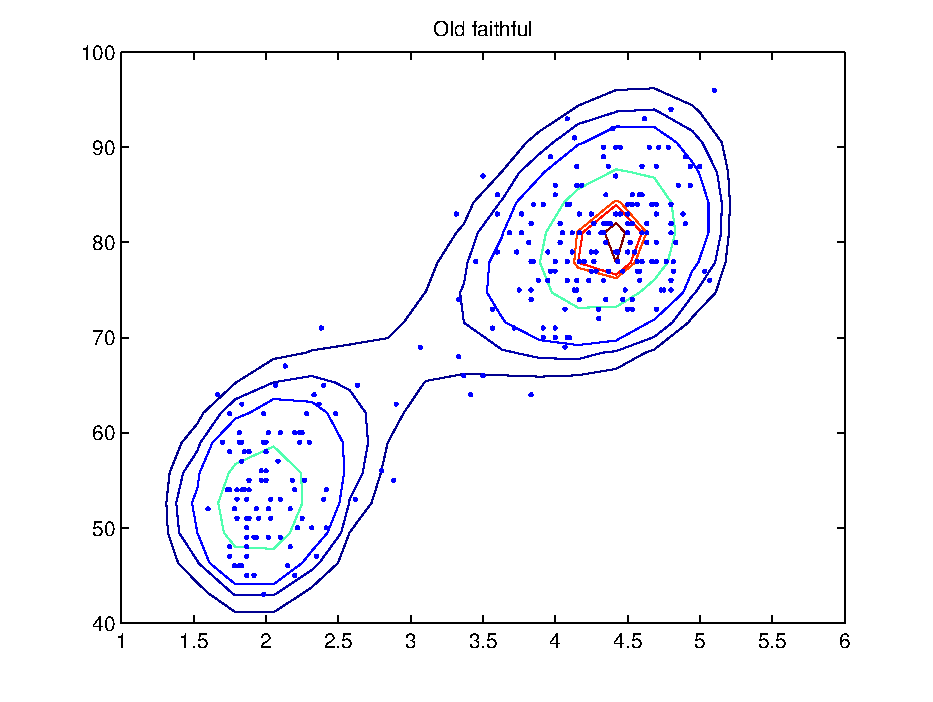
\includegraphics[width=7cm]{demo_lgpdens_fig2}
    }
    \caption[]{Density estimates for two different distributions. Figures are from \code{demo\_lgpdens}. On the left blue line is density estimation of Galaxy data while gray area is 95\% mean region and on the right is 2D density estimation with countours based on Old faithful data.}\label{fig_demo_lgpdens}
  \end{center}
\end{figure}

%    The likelihood is defined as follows:
%               __ n
%      p(y|f) = || i=1 exp(f_i) / Sum_{j=1}^n exp(f_j),
%
%      where f contains latent values.


%    LIK = LIK_LGPC creates a logistic Gaussian process likelihood
%    structure for conditional density estimation
%
%    The likelihood contribution for the $k$th conditional slice 
%    is defined as follows:
%                   __ n
%      p(y_k|f_k) = || i=1 exp(f_ki) / Sum_{j=1}^n exp(f_kj),
%
%      where f contains latent values.

\subsection{Input dependent models}

In input-dependent models more than one latent variables are used for modeling different parameters of the distribution. Additional latent variables in turn enable modeling dependencies between inputs and parameters. 

\subsubsection{Input-dependent Noise}
Input-dependent noise model \citep{Goldberg:1997} can be used to model
regression data. The model assumes Gaussian distributed data with
latent variables defining both mean and variance of the Gaussian
distribution instead of just the mean like in the standard Gaussian
likelihood. Setting independent GP priors for the two latent
variables, it is possible to infer non-constant noise,
e.g. input-dependent, in the data.

The likelihood is defined as
\begin{align}
  p(\y|\f^{(1)}, \f^{(2)}, \sigma^2)=\prod_{i=1}^n N(y_i | f_i^{(1)}, \sigma^2 \exp(f_i^{(2)})),
\end{align}
with latent function $f^{(1)}$ defining the mean and $f^{(2)}$
defining the variance. Input-dependent noise is demonstrated in
\code{demo\_inputdependentnoise} with both heteroscedastic and
constant noise.
% missing description

\subsubsection{Input-dependent overdispersed Weibull}
In input-dependent Weibull model additional latent variable is used for modeling shape parameter $r$ of the standard Weibull model. 

The likelihood is defined as
\begin{eqnarray}
 p( \y |\f^{(1)}, \f_i^{(2)},\mathbf{z}) =&& \prod_{i=1}^n \exp(f_i^{(2)})^{1-z_i} \exp \Big{(} (1-z_i)f^{(1)}_i \\ \nonumber
 &+&(1-z_i)(\exp(f_i^{(2)})-1)\log(y_i)\exp(f^{(1)}_i)y_i^{\exp(f_i^{(2)})} \Big{)}, \nonumber
\end{eqnarray}
where $\mathbf{z}$ is a vector of censoring indicators with $z_i = 0$ for
uncensored event and $z_i = 1$ for right censored event for
observation $i$. Latent variable $f_2$ is used for modeling the shape parameter here. Because the dispersion parameter is constrained to be greater than 0, it must be computed through $\exp(f_2)$ to ensure positiveness. Input-dependent Weibull is demonstrated in \code{demo\_inputdependentweibull}.

\subsection{Monotonicity constraint}
\label{sec_monotonic}.

\citet{Riihimaki+Vehtari:2010} presented how a monotonicity constraint
for GP can be introduced with virtual derivative observations, and
the resulting posterior can be approximated with expectation
propagation.

Currently GPstuff supports monotonicity constraint for models which
have Gaussian likelihood or fully factoring likelihoods with EP
inference and which use covariance functions \code{gpcf\_constant},
\code{gpcf\_linear} and
\code{gpcf\_sexp}. \citet{Riihimaki+Vehtari:2010} used type II MAP
estimate for the hyperparameters, but GPstuff allows easy integration
over the hyperparameters with any method described in
Section~\ref{sec_marginalization_over_hyperparam}.

GP model with monotonicity constraint can be easily constructed with
the function \code{gp\_monotonic}. Monotonicity constraint is
demonstrated in \code{demo\_monotonic} and \code{demo\_monotonic2}.

Figure~\ref{monotonicity} displays the predictions with models with
and without the monotonicity constraint. The monotonicity constraint
allows inclusion of sensible prior information that death rate
increases as age increases. The effect is shown most clearly for
larger ages where there is less observations, but also overall reduction in
uncertainty related to the latent function can be seen.

\begin{figure}
  \begin{center}       
      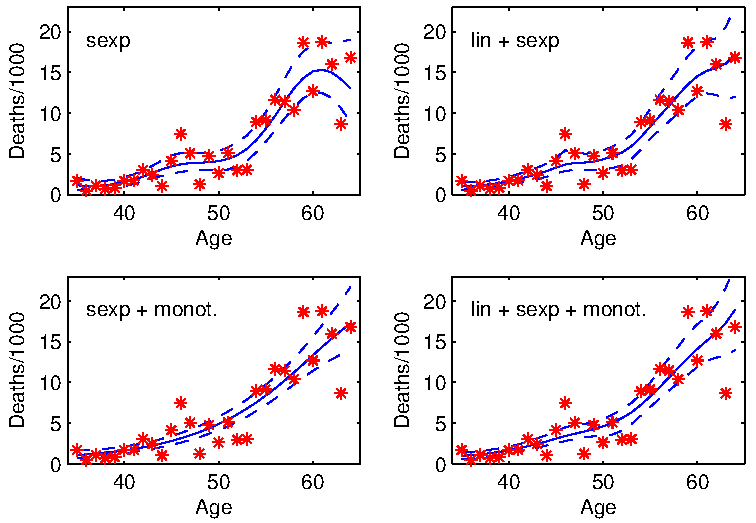
\includegraphics[]{demo_monotonic2_fig1.pdf}  
    \end{center}\caption{Illustration how the monotonicity constraint
      of the latent function affects the predictions. Mortality rate
      data from \citet{Broffitt:1988}.}
  \label{monotonicity} 
\end{figure}

\section{Mean functions}
\label{cha:mean-functions}

In the standard GP regression a zero mean function is assumed for
the prior process. This is convenient but there are nonetheless
some advantages in using a specified mean function. The basic
principle in doing GP regression with a mean function is to apply a
zero mean GP for the difference between observations and the mean
function.

\subsection{Explicit basis functions}

Here we follow closely the presentation of
\citep{Rasmussen+Williams:2006} about the subject and briefly
present the main results. A mean function can be specified as a
weighted sum of some basis functions $h$
% 
\begin{equation}
  \textbf{m} = \textbf{h}(\textbf{x})^\top \boldsymbol{\beta},   \nonumber
\end{equation}
% 
with weights $\boldsymbol{\beta}$. The target of modeling, the underlying process \textbf{g}, is assumed to be a sum of mean function and a zero mean GP. 
% 
\begin{equation}
  \textbf{g} = \textbf{h}(\textbf{x})^\top \boldsymbol{\beta} + \mathcal{GP}(0,\textbf{K}).	\nonumber
\end{equation}
% 
By assuming Gaussian prior for the weights $\boldsymbol{\beta} \sim \mathcal{N}(\textbf{b},\textbf{B}),\nonumber$ the weight parameters can be integrated out and the prior for \textbf{g} is another GP
% 
\begin{equation}
  \label{GP_mean_prior}
  \emph{prior}\; \textbf{g} \sim \mathcal{GP}\left(\,\textbf{h}(\textbf{x})^\top \textbf{b},\,\textbf{K} + 
    \textbf{h}(\textbf{x})^\top \textbf{B}\,\textbf{h}(\textbf{x})\,\right). \nonumber
\end{equation}
% 
The predictive equations are obtained by using the mean and covariance of the prior \eqref{GP_mean_prior} in the zero mean GP predictive equations \eqref{eq_posterior_in_gaussian_case}
% 
\begin{eqnarray}
  \label{gp_mean_predE}
  \mathbb{E(\textbf{g}_*)} &=& \mathbb{E(\textbf{f}_*)} + \textbf{R}^\top \boldsymbol{\overline{\beta}},	\\
  \label{gp_mean_predV}\COV(\textbf{g}_*) &=& \COV(\textbf{f}_*) + \textbf{R}^\top\left( \textbf{B}^{-1} + 
    \textbf{H}\textbf{K}_{y}^{-1}\textbf{H}^\top \right)\textbf{R},	\\
  \nonumber\\
  &\boldsymbol{\overline{\beta}}& = 
  \left( \textbf{B}^{-1} + \textbf{H}\textbf{K}_y^{-1}\textbf{H}^\top \right)^{-1} 
  \left( \textbf{B}^{-1}\textbf{b} + \textbf{H}\textbf{K}_y^{-1}\textbf{y}\right), \nonumber\\
  &\textbf{R}& = \textbf{H}_* - \textbf{H}\textbf{K}_y^{-1}\textbf{K}_*,\nonumber\\
  &\textbf{H}& = 	\left[\begin{array}{c}
      h_1(\textbf{x})\\
      h_2(\textbf{x}) \\
      \vdots\\
      h_k(\textbf{x})
    \end{array}\right],\,  \textit{\textbf{x} is row vector}.\nonumber
\end{eqnarray}
% 
If the prior assumptions about the weights are vague then $\textbf{B}^{-1} \rightarrow O$, ($O$ is a zero matrix) and the predictive 
equations \eqref{gp_mean_predE} and \eqref{gp_mean_predV} don't depend on $\textbf{b}$ or $\textbf{B}$
% 
\begin{eqnarray}
  \label{gp_mean_predEvague}
  \mathbb{E(\textbf{g}_*)} &=& \mathbb{E(\textbf{f}_*)} + \textbf{R}^\top \boldsymbol{\overline{\beta}_v},\\
  \label{gp_mean_predVvague}\COV(\textbf{g}_*) &=& \COV(\textbf{f}_*) + \textbf{R}^\top\left( 
    \textbf{H}\textbf{K}_{y}^{-1}\textbf{H}^\top \right)\textbf{R},	\\
  \nonumber\\
  &\boldsymbol{\overline{\beta}_v}& = 
  \left(\textbf{H}\textbf{K}_y^{-1}\textbf{H}^\top \right)^{-1} 
  \textbf{H}\textbf{K}_y^{-1}\textbf{y}, \nonumber
\end{eqnarray}
% 
Corresponding the exact and vague prior for the basis functions' weights there are two versions of the marginal likelihood.
With exact prior the marginal likelihood is
% 
\begin{eqnarray}
  \log p(\textbf{y} \mid \textbf{X}, \textbf{b}, \textbf{B}) &=& -\frac{1}{2}\textbf{M}^\top \textbf{N}^{-1}\textbf{M} 
  -\frac{1}{2}\log|\textbf{K}_y|  -\frac{1}{2}\log|\textbf{B}|-\frac{1}{2}\log|\textbf{A}| -\frac{n}{2}\log 2\pi,\nonumber\\
  \textbf{M} &=& \textbf{H}^\top\textbf{b}-\textbf{y} ,\nonumber\\
  \textbf{N} &=& \textbf{K}_y  + \textbf{H}^\top \textbf{B}\textbf{H},\nonumber\\
  \textbf{A} &=& \textbf{B}^{-1} + \textbf{H}\textbf{K}_y^{-1}\textbf{H}^\top ,\nonumber
\end{eqnarray}
% 
where $n$ is the amount of observations. Its derivative with respect to hyperparameters are
% 
\begin{eqnarray}
  \frac{\partial }{\partial \theta_i} \log p(\textbf{y} \mid \textbf{X}, \textbf{b}, \textbf{B}) = &+&\frac{1}{2} 
  \textbf{M}^\top\textbf{N}^{-1}\frac{\partial \textbf{K}_y}{\partial \theta_i}\textbf{N}^{-1}\textbf{M}^\top \nonumber\\
  &-&\frac{1}{2}\text{tr}\left(\textbf{K}_y^{-1} \frac{\partial \textbf{K}_y}{\partial \theta_i}\right) - \frac{1}{2}\text{tr}\left(\textbf{A}^{-1} \frac{\partial \textbf{A}}{\partial \theta_i} \right), \nonumber\\
  \frac{\partial \textbf{A}}{\partial \theta_i} =&-&\textbf{H}\textbf{K}_y^{-1}\frac{\partial \textbf{K}_y}{\partial \theta_i}\textbf{K}_y^{-1}\textbf{H}^\top. 		\nonumber
  % 
\end{eqnarray}
% 
With a vague prior the marginal likelihood is 
% 
\begin{eqnarray}
  \log p(\textbf{y} \mid \textbf{X}) = &-&\frac{1}{2}\textbf{y}^\top \textbf{K}_y^{-1}\textbf{y} 
  + \frac{1}{2}\textbf{y}^\top \textbf{C}\textbf{y}			\nonumber\\
  &-&\frac{1}{2}\log |\textbf{K}_y|-\frac{1}{2}\log |\textbf{A}_v|
  -\frac{n-m}{2}\log 2\pi, 						\nonumber\\
  \textbf{A}_v = && \textbf{H}\textbf{K}_y^{-1}\textbf{H}^\top			\nonumber\\
  \textbf{C} =&& \textbf{K}_y^{-1}\textbf{H}^\top\textbf{A}_v^{-1}\textbf{H}\textbf{K}_y^{-1}, \nonumber
\end{eqnarray}
% 
where $m$ is the rank of $H^\top$. Its derivative is
\begin{eqnarray}
  \label{gp_mean_marglikeli_pvag_der}
  \frac{\partial }{\partial \theta_i} \log p(\textbf{y} \mid \textbf{X})
  = &&\frac{1}{2}\textbf{y}^\top \textbf{P}\textbf{y}
  +\frac{1}{2}\left(-\textbf{y}^\top\textbf{P}\textbf{G}
    -\textbf{G}^\top\textbf{P}\textbf{y}
    +\textbf{G}^\top\textbf{P}\textbf{G}\right)\\
  &-&\frac{1}{2}\text{tr}\left(\textbf{K}_y^{-1} \frac{\partial
      \textbf{K}_y}{\partial \theta_i} \right) -
  \frac{1}{2}\text{tr}\left(\textbf{A}_v^{-1} \frac{\partial
      \textbf{A}_v}{\partial \theta_i} \right),        \nonumber\\
  \textbf{P} &=&    \textbf{K}_y^{-1} \frac{\partial \textbf{K}_y}{\partial
    \theta_i}\textbf{K}_y^{-1},\nonumber\\
  \textbf{G}
  &=&    \textbf{H}^\top\textbf{A}^{-1}\textbf{H}\textbf{K}_y^{-1}\textbf{y},    \nonumber
\end{eqnarray} 
% 
where has been used the fact that matrices $\textbf{K}_y^{-1}$,
$\frac{\partial \textbf{K}_y}{\partial \theta_i}$ and $\textbf{A}_v$
are symmetric. The above expression
\eqref{gp_mean_marglikeli_pvag_der} could be simplified a little
further because $\textbf{y}^\top\textbf{P}\textbf{G}
+\textbf{G}^\top\textbf{P}\textbf{y} = 2\cdot
\textbf{y}^\top\textbf{P}\textbf{G}$. The use of mean functions is
demonstrated in \code{demo\_regression\_meanf}.

% \subsection{Mean functions in GPstuff: demo\_regression\_meanf}
% \label{sec:meanf}

% Here we will demonstrate, with the
% \code{demo\_regression\_meanf}, how to use mean functions with
% GPstuff. GP regression is done for artificial one dimensional data
% with full GP model and gaussian likelihood. In this presentation
% only the lines of code are presented which are relevant in the mean
% function context. Otherwise this demonstration follows closely
% \code{demo\_regression1}.

% After creating the data and initializing the covariance and
% likelihood functions we are ready to initialize the GP structure.
% The basis functions for mean are given in a cell array of mean
% function structures (note the similarity to the use of covariance
% function structures). 
% \scriptsize
% \begin{verbatim}
% % Create covariance and likelihood structures
% gpcf = gpcf_sexp('lengthScale', [0.5], 'magnSigma2', .5);
% lik = lik_gaussian('sigma2', 0.4^2);

% % Initialize base functions for GP's mean function.
% gpmf1 = gpmf_constant('prior_mean',.3,'prior_cov',1);
% gpmf2 = gpmf_linear('prior_mean',.3,'prior_cov',1);
% gpmf3 = gpmf_squared('prior_mean',.3,'prior_cov',1);

% % Initialize gp structure
% gp = gp_set('lik', lik, 'cf', {gpcf}, 'meanf', {gpmf1,gpmf2,gpmf3});
% \end{verbatim}
% \normalsize

% In figure \ref{demo_meanFunc_fig1} is presented the underlying
% process, the GP prediction, the used mean function, 95\,\%
% confidence interval and the observations.
% %
% \begin{figure}[htb]
% \centering
% \includegraphics[width=5.3cm]{demo_meanFuncs_fig1}
% \caption{GP prediction for the process f with a mean function.}
% \label{demo_meanFunc_fig1}
% \end{figure}

\section{Sparse Gaussian processes}
\label{cha:sparse-GP}

%foo

The evaluation of the inverse and determinant of the covariance matrix
in the log marginal likelihood (or its approximation) and its gradient
scale as $O(n^3)$ in time. This restricts the implementation of GP
models to moderate size data sets. However, the unfavorable scaling in
computational time can be alleviated with sparse approximations to GP
and compactly supported (CS) covariance functions. The sparse
approximations scale as $O(nm^2)$, where $m<n$ and the CS covariance
functions lead to computations which scale, in general, as $O(n^3)$
but with a smaller constant than with traditional globally supported
covariance functions. Many sparse GPs are proposed in the literature
and some of them are build into \pkg{GPstuff}.

\subsection{Compactly supported covariance functions}

%foo

A CS covariance function gives zero correlation between data points
whose distance exceeds a certain threshold. This leads to a sparse
covariance matrix. The challenge with constructing CS covariance
functions is to guarantee their positive definiteness and much
literature has been devoted on the subject \citep[see
e.g.][]{Sanso+Schuh:1987,Wu:1995,Wendland:1995,Gaspari+Cohn:1999,Gneiting:1999,Gneiting:2002,Buhmann:2000}
The CS functions implemented in \pkg{GPstuff} are Wendland's piecewise
polynomials $k_{\text{pp},q}$ \citep{Wendland:2005}, such as
% 
\begin{equation}\label{ppcs2}
k_{\text{pp},2} = 
\frac{\sigma_{\text{pp}}^2}{3} (1 - r)_+^{j+2} \left( (j^2 + 4j
   +3) r^2  +   (3j + 6)r + 3\right) , 
\end{equation}
%
where $j = \lfloor d/2 \rfloor + 3$. These functions correspond to
processes that are $q$ times mean square differentiable and are
positive definite up to an input dimension $d$. Thus, the degree of
the polynomial has to be increased alongside the input dimension. The
dependence of CS covariance functions to the input dimension is very
fundamental. There are no radial CS functions that are positive
definite on every $\Re^d$ \citep[see e.g.][theorem
9.2]{Wendland:1995}.

The key idea with CS covariance functions is that, roughly speaking,
only the nonzero elements of the covariance matrix are used in the
calculations. This may speed up the calculations substantially since
in some situations only a fraction of the elements of the covariance
matrix are non-zero \citep[see
e.g.][]{Vanhatalo+Vehtari:2008,Rue+Martino+Chopin:2009}. In practice,
efficient sparse matrix routines are needed \citep{Davis:2006}. These
are nowadays a standard utility in many statistical computing packages
or available as an additional package for them.  \pkg{GPstuff}
utilizes the sparse matrix routines from \pkg{SuiteSparse} written by
Tim Davis (\url{http://www.cise.ufl.edu/research/sparse/SuiteSparse/})
and this package should be installed before using CS covariance
functions.

The CS covariance functions have been rather widely studied in the
geostatistics applications \citep[see
e.g.][]{Gneiting:2002,Furrer+Genton+Nychka:2006,Moreaux:2008}. There
the computational speed-up relies on efficient linear solvers for the
predictive mean $[\tilde{\f}] = \Kaf (\Kff +\sigma^2)^{-1}\y$. The
parameters are either fitted to the empirical covariance, optimized
using a line search in one dimension
\citep{Kaufman+Schervish+Nychka:2008} or sampled with Metropolis
Hastings. The benefits from a sparse covariance matrix have been
immediate since the problems collapse to solving sparse linear
systems. However, utilizing the gradient of the log posterior of the
parameters, as is done in \pkg{GPstuff} needs extra sparse matrix
tools. These are introduced and discussed by
\citet{Vanhatalo+Vehtari:2008}.  EP algorithm requires also special
considerations with CS covariance functions. The posterior covariance
in EP \eqref{eq_posterior_in_EP_case} does not remain sparse, and
thereby it has to be expressed implicitly. This issue is discussed by
\citet{Vanhatalo+Vehtari:2010} and
\citet{Vanhatalo+Pietilainen+Vehtari:2010}.

\subsubsection{Compactly supported covariance functions in GPstuff}

The demo \code{demo\_regression\_ppcs} contains a regression example
with CS covariance function $k_{\text{pp},2}$ (\code{gpcf\_ppcs2}).
The data contain US annual precipitation summaries from year 1995 for
5776 observation stations. The user interface of \pkg{GPstuff} makes
no difference between globally and compactly supported covariance
functions but the code is optimized to use sparse matrix routines
whenever the covariance matrix is sparse.  Thus, we can construct the
model, find the MAP estimate for the parameters and predict to new
input locations in a familiar way:
%
\begin{verbatim}
pn = prior_t('nu', 4, 's2', 0.3);
lik = lik_gaussian('sigma2', 1, 'sigma2_prior', pn);
pl2 = prior_gamma('sh', 5, 'is', 1);
pm2 = prior_sqrtt('nu', 1, 's2', 150);
gpcf2 = gpcf_ppcs2('nin', nin, 'lengthScale', [1 2], 'magnSigma2', 3, ...
                   'lengthScale_prior', pl2, 'magnSigma2_prior', pm2);
gp = gp_set('lik', lik, 'cf', gpcf2, 'jitterSigma2', 1e-6);
gp = gp_optim(gp,x,y,'opt',opt);
Eft = gp_pred(gp, x, y, xx);
\end{verbatim}
%
With this data the covariance matrix is rather sparse since only about
5\% of its elements are non-zero. The structure of the covariance
matrix is plotted after the approximate minimum degree (AMD)
permutation \citep{Davis:2006} in Figure~\ref{demo_ppcsCov}. The demo
\code{demo\_spatial2} illustrates the use of compactly supported
covariance functions with a non-Gaussian likelihood.

\begin{figure}[]
    \begin{center}
      \subfigure[The nonzero elements of $\Kff$.]{
        \label{}
        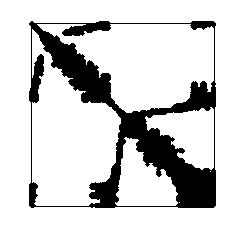
\includegraphics[width=3.2cm]{demo_ppcsCov1}
      }
      \hspace{-8mm}
      ~
      \subfigure[The posterior predictive mean surface.]{ 
        \label{}
        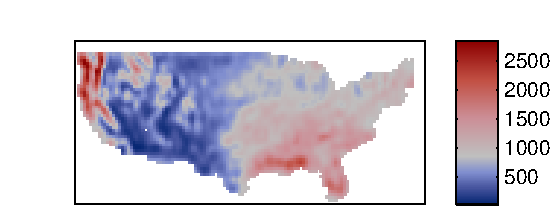
\includegraphics[width=9cm]{demo_ppcsCov2}
       }
       \caption[]{The nonzero elements of $\Kff$ with
         $k_{\text{pp,2}}$ function, and the posterior predictive mean
         of the latent function in the US precipitation data
         set.}\label{demo_ppcsCov}
    \end{center}
\end{figure}


\subsection{FIC and PIC sparse approximations}\label{FIC_PICsparse_approximations}

\citet{Snelson+Ghahramani:2006} proposed a sparse pseudo-input GP
(SPGP), which \citet{Quinonero-Candela+Rasmussen:2005} named later
fully independent conditional (FIC).
%  The original idea in SPGP was that the
% sparse approximation is used only in the training phase and
% predictions are conducted using the exact covariance matrix, where the
% word 'training' comes to the name. If the approximation is used also
% for the predictions, the word training should drop out leading to FIC.
The partially independent conditional (PIC) sparse approximation is an
extension of FIC
\citep{Quinonero-Candela+Rasmussen:2005,Snelson+Ghahramani:2007a}, and
they are both treated here following
\citet{Quinonero-Candela+Rasmussen:2005}. See also
\citep{Vanhatalo+Vehtari:2008,Vanhatalo+Pietilainen+Vehtari:2010} for
further discussion. The approximations are based on introducing an
additional set of latent variables $\uu = \{u_i \}_{i=1}^{m}$, called
\emph{inducing variables}. These correspond to a set of input
locations $\mb{X}_{u}$, called \emph{inducing inputs}. The latent
function prior is approximated as
%
\begin{equation}\label{cond_independ_joint_prior}   %jätä
  p(\f|\mb{X}, \theta) \approx q(\f | \mb{X}, \mb{X}_{u}, \theta) = \int q(\f |
  \mb{X}, \mb{X}_{u}, \uu, \theta)p(\uu | \mb{X}_{u}, \theta)\mathrm{d}\mathbf{u},
\end{equation}
%
where $q(\f|\mb{X}, \mb{X}_{u}, \uu, \theta)$ is an inducing
conditional. The above decomposition leads to the exact prior if the
true conditional $\f | \mb{X}, \mb{X}_{u}, \uu, \theta \sim \N(\Kfu \iKuu\uu,
\Kff-\mb{K}_{\text{f,u}} \iKuu \mb{K}_{\text{u,f}})$ is used. However,
in FIC framework the latent variables are assumed to be conditionally
independent given $\uu$, in which case the inducing conditional
factorizes $q(\f | \mb{X}, \mb{X}_{u}, \uu, \theta)\!= \prod q_i(f_i|\mb{X}, \mb{X}_{u}, \uu, \theta)$. In PIC latent
variables are set in blocks which are conditionally independent of
each others, given $\uu$, but the latent variables within a block have
a multivariate normal distribution with the original covariance. The
approximate conditionals of FIC and PIC can be summarized as
%
\begin{equation}
q(\f | \mb{X}, \mb{X}_{u}, \uu, \theta, \mb{M}) = \N(\f|\Kfu \iKuu\uu,
\mathrm{mask}\left(\Kff-\mb{K}_{\text{f,u}} \iKuu
\mb{K}_{\text{u,f}}|\mb{M}\right)), 
\end{equation}
%
where the function $\LL=\mathrm{mask}\left(\cdot|\mb{M}\right)$, with
matrix $\mb{M}$ of ones and zeros, returns a matrix $\LL$ of size
$\mb{M}$ and elements $\LL_{ij} = [\cdot]_{ij}$ if $\mb{M}_{ij} = 1$
and $\LL_{ij} =0$ otherwise.  An approximation with $\mb{M} = \mb{I}$
corresponds to FIC and an approximation where $\mb{M}$ is block
diagonal corresponds to PIC.  The inducing variables are given a
zero-mean Gaussian prior $\uu|\theta,\mb{X}_u\sim \N(\mb{0},\Kuu)$ so
that the approximate prior over latent variables is
%
\begin{equation}
  q(\f | \mb{X}, \mb{X}_{u},\theta,\mb{M}) = \N(\f | \mb{0}, \mb{K}_{\text{f,u}} \iKuu\mb{K}_{\text{u,f}}+\LL).
\label{GP_FITC_prior}
\end{equation}
%
The matrix $\mb{K}_{\text{f,u}} \iKuu\mb{K}_{\text{u,f}}$ is of
rank $m$ and $\LL$ is a rank $n$ (block) diagonal matrix. The prior
covariance above can be seen as a non-stationary covariance function of its
own 
% %
% \begin{equation}\label{PIC_covariance}
% k_{\text{FIC/PIC}}(k(x_i,x_j|\theta),\mb{M},\mb{X}_{u}) = 
% \begin{cases} 
%    k(\x_i,\x_j) & \text{if $\mb{M}_{ij}=1$}, \\
%    \left[\Kfu \iKuu\Kuf\right]_{ij} &
%   \text{otherwise},
% \end{cases} 
% \end{equation}
% %
where the inducing inputs $\mb{X}_u$ and the matrix $\mb{M}$ are free
parameters similar to parameters, which can be optimized
alongside $\theta$ \citep{Snelson+Ghahramani:2006,Lawrence:2007}.

The computational savings are obtained by using the
Woodbury-Sherman-Morrison lemma \citep[e.g.][]{Harville:1997} to
invert the covariance matrix in \eqref{GP_FITC_prior} as
%
\begin{equation}\label{Woodbury_eq}
(\mb{K}_{\text{f,u}} \iKuu\mb{K}_{\text{u,f}}+\LL)^{-1} = \LL^{-1} -
\mb{V}\mb{V}^{\text{T}},
\end{equation}
%
where $\mb{V} =\LL^{-1}\Kfu \text{chol}[(\Kuu
+\Kuf\LL^{-1}\Kfu)^{-1}]$. There is a
similar result also for the determinant. With FIC the computational
time is dominated by the matrix multiplications, which need time
$O(m^2n)$. With PIC the cost depends also on the sizes of the blocks
in $\LL$. If the blocks were of equal size $b\times b$, the time for
inversion of $\LL$ would be $O(n/b\times b^3)=O(nb^2)$. With blocks at
most the size of the number of inducing inputs, that is $b=m$, the
computational cost in PIC and FIC are similar. PIC approaches FIC in
the limit of a block size one and the exact GP in the limit of a block
size $n$ \citep{Snelson:2007b}.

\subsubsection{FIC sparse approximation in GPstuff}

The same data that were discussed in the section
\ref{sec:demo_regression1} is analyzed with sparse approximations in
the demo \code{demo\_regression\_sparse1}. The sparse approximation is
a property of the GP structure and we can construct the model
similarly to the full GP models:
%
\begin{verbatim}
gp_fic = gp_set('type', 'FIC', 'lik', lik, 'cf', gpcf, 'X_u', X_u)
\end{verbatim}
%
The difference is that we have to define the type of the sparse
approximation, here \verb|'FIC'|, and set the inducing inputs
\code{X\_u} in the GP structure. Since the inducing inputs are
considered as extra parameters common to all of the covariance
functions (there may be more than one covariance function in additive
models) they are set in the GP structure instead of the covariance
function structure. If we want to optimize the inducing inputs
alongside the parameters they need to have a prior as well.  GP
structure initialization gives them a uniform prior by default.

We can optimize all the parameters, including the inducing inputs, as
with a full GP. Sometimes, for example in spatial problems, it is
better to fix the inducing inputs
\citep{Vanhatalo+Pietilainen+Vehtari:2010} or it may be more efficient
to optimize the parameters and inducing inputs separately, so that we
iterate the separate optimization steps until convergence
(demonstrated in \code{demo\_regression\_sparse1}).  The parameters to
be optimized are defined by the field \code{infer\_params} in the GP
structure. This field regulates which parameters are considered fixed
and which are inferred in the group level (covariance function,
inducing inputs, likelihood).  We may also want to fix one of the
parameters inside these groups. For example, covariance function
magnitude.  If this is the case, then the parameter to be fixed should
be given an empty prior (\code{prior\_fixed}). If the parameter has a
prior structure it is an indicator that we want to infer that
parameter.
 
\subsubsection{PIC sparse approximation in GPstuff}\label{sec:PIC_regression}

In PIC, in addition to defining the inducing inputs, we need to appoint
every data point in a block. The block structure is common to all
covariance functions, similarly to the inducing inputs, for which reason
the block information is stored in the GP structure. After the
blocking and initialization of the inducing inputs the GP structure is
constructed as follows:
%
\begin{verbatim}
gp_pic = gp_set('type','PIC','lik',lik,'cf',gpcf,'X_u',X_u,'tr_index',trindex);
\end{verbatim}
%
Above, the cell array \code{trindex} contains the block index vectors
for training data. It means that, for example, the inputs and outputs
\code{x(trindex\{i\},:)} and \code{y(trindex\{i\},:)} belong to the
i'th block. The optimization of parameters and inducing inputs is
done the same way as with FIC or a full GP model. In prediction,
however, we have to give one extra input, \code{tstindex}, for
\code{gp\_pred}. This defines how the prediction inputs are appointed
in the blocks in a same manner as \code{trindex} appoints the training
inputs. 
%
\begin{verbatim}
Eft_pic = gp_pred(gp_pic, x, y, xt, 'tstind', tstindex);
\end{verbatim}
%
\subsection{Deterministic training conditional, subset of regressors and
  variational sparse approximation}


The deterministic training conditional is based on the works by
\citet{Csato+Opper:2002} and \citet{Seeger+Williams+Lawrence:2003} and
was earlier called Projected Latent Variables \citep[see][for
more details]{Quinonero-Candela+Rasmussen:2005}. The approximation 
can be constructed similarly as FIC and PIC by defining the inducing
conditional, which in the case of DTC is 
%
\begin{equation}
q(\f | \mb{X}, \mb{X}_{u}, \uu, \theta) = \N(\f|\Kfu \iKuu\uu,0).
\end{equation}
%
This implies that the approximate prior over latent variables is
%
\begin{equation}
  q(\f | \mb{X}, \mb{X}_{u}, \theta) = \N(\f | \mb{0}, \mb{K}_{\text{f,u}} \iKuu\mb{K}_{\text{u,f}}).
\label{GP_DTC_prior}
\end{equation}
%
The deterministic training conditional is not strictly speaking a
proper GP since it uses different covariance function for the latent
variables appointed to the training inputs and for the latent
variables at the prediction sites, $\tilde{f}$. The prior covariance
for $\tilde{f}$ is the true covariance $\Kaa$ instead of
$\Kau\iKuu\Kua$. This does not affect the predictive mean since the
cross covariance $\COV[\f,\tilde{\f}] = \Kfu\iKuu\Kua$, but it gives a
larger predictive variance. An older version of DTC is the subset of
regressors (SOR) sparse approximation which utilizes $\Kau\iKuu\Kua$.
However, this resembles a singular Gaussian distribution and thus the
predictive variance may be negative. DTC tries to fix this problem by
using $\Kaa$ \citep[see][]{Quinonero-Candela+Rasmussen:2005}. DTC and
SOR are identical in other respects than in the predictive variance
evaluation. In spatial statistics, SOR has been used by
\citet{Banerjee+Gelfand+Finley+Sang:2008} with a name Gaussian
predictive process model.

The approximate prior of the variational approximation by
\citet{Titsias:2009} is exactly the same as that of DTC. The
difference between the two approximations is that in the variational
setting the inducing inputs and covariance function parameters are
optimized differently. The inducing inputs and parameters can be seen
as variational parameters that should be chosen to maximize the
variational lower bound between the true GP posterior and the sparse
approximation. This leads to optimization of modified log marginal
likelihood
%
\begin{equation}
V(\theta, \mb{X}_u) = \log [N(\y|0, \sigma^2\mb{I} + \Qff) ] -
\frac{1}{2\sigma^2} \text{tr}(\Kff - \Kfu\iKuu\Kuf)
\end{equation}
%
with Gaussian likelihood. With non-Gaussian likelihood, the
variational lower bound is similar but $\sigma^2\mb{I}$ is replaced by
$\mb{W}^{-1}$ (Laplace approximation) or $\tilde{\mb{\Sigma}}$ (EP).


\subsubsection{Variational, DTC and SOR sparse approximation in GPstuff}

%foo

The variational, DTC and SOR sparse approximations are constructed
similarly to FIC. Only the type of the GP changes:
%
\begin{verbatim}
gp_var = gp_set('type', 'VAR', 'lik', lik, 'cf', gpcf, 'X_u', X_u);
gp_dtc = gp_set('type', 'DTC', 'lik', lik, 'cf', gpcf, 'X_u', X_u);
gp_sor = gp_set('type', 'SOR', 'lik', lik, 'cf', gpcf, 'X_u', X_u);
\end{verbatim}
%
The sparse GP approximations are compared in the demo
\code{demo\_regression\_sparse2}, and, for example,
\citet{Quinonero-Candela+Rasmussen:2005}, \citet{Snelson:2007b},
\citet{Titsias:2009}, and \citet{Alvarez+Luengo+Titsias+Lawrence:2010}
treat them in more detail.


\subsection{Sparse GP models with non-Gaussian likelihoods}

The extension of sparse GP models to non-Gaussian likelihoods is
straightforward in \pkg{GPstuff}. User can define the sparse GP just
as described in the previous two sections and then continue with the
construction of likelihood exactly the same way as with a full GP.
The Laplace approximation, EP and integration methods can be used with
the same commands as with full GP. This is demonstrated in
\code{demo\_spatial1}.

\subsection{Predictive active set selection for classification}

Predictive active set selection for Gaussian processes \citep[PASS-GP,
][]{Henao+Winther:2012} is a sparse approximation for classification
models. PASS-GP uses predictive distributions to estimate which data
points to include in the active set, so that it will include points
with potentially high impact to the classifier decision process while
removing those that are less relevant.
%
Function \code{passgp} accepts classification GP with latent method
set to EP or Laplace, and selects the active set and optimises the
hyperparameters. Its use is demonstrated in \code{demo\_passgp}.

\section{Modifying the covariance functions}\label{sec:modifying_covariance}

\subsection{Additive models}\label{sec_additive_models}

In many practical situations, a GP prior with only one covariance
function may be too restrictive since such a construction can model
effectively only one phenomenon. For example, the latent function may
vary rather smoothly across the whole area of interest, but at the
same time it can have fast local variations. In this case, a more
reasonable model would be $f(\mb{x}) = g(\mb{x}) + h(\mb{x})$, where
the latent value function is a sum of two functions, slow and fast
varying. By placing a separate GP prior for both of the functions $g$
and $h$ we obtain an additive prior
%
\begin{equation}\label{two_length_scale_model}
f(\x)|\theta \sim \GP(0,k_g(\x,\x') + k_h(\x,\x')).
\end{equation}
%
The marginal likelihood and posterior distribution of the latent
variables are as before with $\Kff = \mb{K}_{\text{g,g}} +
\mb{K}_{\text{h,h}}$. However, if we are interested on only, say,
phenomenon $g$, we can consider the $h$ part of the latent function as
correlated noise and evaluate the predictive distribution for $g$,
which with the Gaussian likelihood would be
%
\begin{equation}
  \tilde{g}(\tilde{\x})|\mathcal{D},
  \theta \sim \GP\left(k_g(\tilde{\x},\mb{X})(\Kff + \sigma^2\mb{I})^{-1}\mb{y}, 
    k_g(\tilde{\x},\tilde{\x}') -
    k_g(\tilde{\x},\mb{X})(\Kff + \sigma^2\mb{I})^{-1}  k_g(\mb{X},\tilde{\x}')\right).
\end{equation}
%
With non-Gaussian likelihood, the Laplace and EP approximations for
this are similar since only $\sigma^2\mb{I}$ and $(\Kff +
\sigma^2\mb{I})^{-1}\mb{y}$ change in the approximations.

The multiple length-scale model can be formed also using specific
covariance functions. For example, a rational quadratic covariance
function (\code{gpcf\_rq}) can be seen as a scale mixture of squared
exponential covariance functions \citep{Rasmussen+Williams:2006}, and
could be useful for data that contain both local and global phenomena.
However, using sparse approximations with the rational quadratic would
prevent it from modeling local phenomena. The additive model
\eqref{two_length_scale_model} suits better for sparse GP formalism
since it enables to combine FIC with CS covariance functions.

As discussed in section \ref{FIC_PICsparse_approximations}, FIC can be
interpreted as a realization of a special kind of covariance function.
\citet{Vanhatalo+Vehtari:2008} proposed to add FIC with CS covariance
function which leads to a latent variable prior
%
\begin{equation}\label{GP_CS+FIC_prior}
\f \mid \mb{X}, \mb{X}_{u}, \theta \sim \N(\mb{0},
\Kfu\iKuu\Kuf+\hat{\LL}),
\end{equation}
%
referred as CS+FIC. Here, the matrix
$\hat{\LL}=\LL+k_{\text{pp,q}}(\mb{X},\mb{X})$ is sparse with the same
sparsity structure as in $k_{\text{pp,q}}(\mb{X},\mb{X})$ and it is
fast to use in computations and cheap to store. 

\subsubsection{Additive models in GPstuff}

The additive models are demonstrated in \code{demo\_periodic} and
\code{demo\_regression\_additive1}. Their construction follows closely the
steps introduced in the previous sections. Consider that we want to
construct a GP with a covariance function that is a sum of squared
exponential and piecewise polynomial $k_{\text{se}}(\x,\x') +
k_{\text{pp},2}(\x,\x')$. In \pkg{GPstuff} this is done as follows:
%
\begin{verbatim}
gpcf1 = gpcf_sexp();
gpcf2 = gpcf_ppcs2('nin', 2);
lik = lik_gaussian('sigma2', 0.1);
gp = gp_set('lik', lik, 'cf', {gpcf1, gpcf2}); 
\end{verbatim}
%
The difference to previous models is that we give more than one
covariance function structure in cell array for the \code{gp\_set}.
The inference with additive model is conducted the same way as
earlier. If we want to make predictions for the two components
$k_{\text{se}}$ and $k_{\text{pp},2}$ independently we can do it by
giving an extra parameter-value pair for the \code{gp\_pred} as
%
\begin{verbatim}
[Ef_sexp, Varf_sexp] = gp_pred(gp, x, y, x, 'predcf', 1);
[Ef_ppcs2, Varf_ppcs2] = gp_pred(gp, x, y, x, 'predcf', 2);
\end{verbatim}

Additive models are constructed analogously with sparse approximations
by changing the type of the GP model. CS+FIC is a special kind of GP
structure and has its own type definition:
%
\begin{verbatim}
gp = gp_set('type', 'CS+FIC', 'lik', lik, 'cf', {gpcf1, gpcf2}, 'X_u', Xu);
\end{verbatim}

It is worth mentioning few things that should be noticed in relation
to sparse approximations. In general, FIC is able to model only
phenomena whose length-scale is long enough compared to the distance
between adjacent inducing inputs.  PIC on the other hand is able to
model also fast varying phenomena inside the blocks. Its drawback,
however, is that the correlation structure is discontinuous which may
result in discontinuous predictions. The CS+FIC model corrects these
deficiencies. In FIC and PIC the inducing inputs are parameters of
every covariance function, which means that all the correlations are
induced through the inducing inputs and the shortest length-scale the
GP is able to model is defined by the locations of the inducing
inputs. In CS+FIC, the CS covariance functions do not utilise inducing
inputs but evaluate the covariance exactly for which reason both the
long and short length-scale phenomena can be captured.  If there are
more than two covariance functions in CS+FIC all the globally
supported functions utilize inducing inputs and all the CS functions
are added to $\hat{\Lambda}$. A detailed treatment on the subject is
given in
\citep[][]{Vanhatalo+Vehtari:2008,Vanhatalo+Vehtari:2010,Vanhatalo+Pietilainen+Vehtari:2010}


\subsection{Additive covariance functions with selected variables}
\label{sec:addit-covar-funct}

In the demo (\code{demo\_regression\_additive2}), we demonstrate how
covariance functions can be modified so that they are functions of
only a subset of inputs. We model an artificial 2D regression data
with additive covariance functions that use only either the first or
second input variable. That is, the covariance is
$k_1(x_1,x_1'|\theta_1) + k_2(x_2,x_2'|\theta_2): \Re^2 \times
\Re^2\mapsto \Re$, where the covariance functions are of type
$k_1(x_1,x_1'|\theta_1): \Re \times \Re \mapsto \Re$. In the example
the covariance is a sum of a squared exponential, which is a function
of the first input dimension $x_1$, and a linear covariance function,
which is a function of the second input dimension $x_2$. The
covariance functions are constructed as follows:
%
\begin{verbatim}
gpcf_s1 = gpcf_sexp('selectedVariables', 1, 'lengthScale',0.5, ...
                    'magnSigma2', 0.15);
gpcf_l2 = gpcf_linear('selectedVariables', 2);
\end{verbatim}
%
The smaller set of inputs is chosen with the field input variable pair
\code{'selectedVariables',1}.

\subsection{Product of covariance functions}

A product of two or more covariance functions $k_1(\x,\x') \cdot
k_2(\x,\x')...$ is a valid covariance function as well. Such
constructions may be useful in situations where the phenomenon is
assumed to be separable. Combining covariance functions into product
form is done with a special covariance function \code{gpcf\_prod}. For
example, multiplying exponential and Mátern covariance functions to
produce separable spatio-temporal model $k(\x,\x') = k_1(x_1,x_1')
\cdot k_2([x_2,x_3]^{\text{T}},[x'_2,x'_3]^{\text{T}})$ where the
temporal component has covariance function $k_1$ and the spatial
components $k_2$ is done as follows:
%
\begin{verbatim}
gpcf1 = gpcf_exp('selectedVariables', 1);
gpcf2 = gpcf_matern32('selectedVariables', [2 3];
gpcf = gpcf_prod('cf', {gpcf1, gpcf2});
\end{verbatim}

The product covariance \code{gpcf\_prod} can also be used to combine
categorical covariance \code{gpcf\_cat} with other covariance
functions to build hierarchical linear and non-linear models, as
illustrated in \code{demo\_regression\_hier}.

% ==========================

\section{State space inference}\label{sec:kalman}
%
{\footnotesize By {Arno Solin}, {Jukka Koskenranta}, and {Simo S{\"a}rkk{\"a}}.\\}

\noindent
For one-dimensional Gaussian processes, instead of directly working with the
usual kernel formalism,$f \sim \mathcal{GP}(0,k(t,t'))$, of the Gaussian
process, certain classes of covariance functions allow to work with the
mathematical dual \citep{Sarkka+Solin+Hartikainen:2013}, where the Gaussian
process is though of as a solution to a $m$th order linear stochastic
differential equation (SDE). The corresponding inference problem can then solved
with Kalman filtering type of methods \citep{Grewal+Andrews:2001,Sarkka:2013},
where the computational complexity is $\mathcal{O}(m^3n)$ making this
formulation beneficial for long (often temporal) data sets.

The state space model corresponding to the GP regression problem can be given as
a linear time-invariant stochastic differential equation of the following form:
%
\begin{align} \label{eq:SDE}
  \begin{split}
  {\mathrm{d} \mathbf{f}(t) \over \mathrm{d} t} 
    &= \mathbf{F} \mathbf{f}(t) + \mathbf{L} \mathbf{w}(t) \\
  y_k 
    &= \mathbf{H} \mathbf{f}(t_k) + \varepsilon_k, 
    \quad \varepsilon_k \sim \mathrm{N}(0,\sigma_\mathrm{n}^2),
  \end{split}
\end{align}
%
where $\mathbf{f}(t) = \begin{pmatrix} f_1(t), f_2(t), \ldots, f_m(t)
\end{pmatrix}^\mathrm{T}$ holds the $m$ stochastic processes, and
$\mathbf{w}(t)$ is a multi-dimensional white noise process with spectral density
$\mathbf{Q}_\mathrm{c}$. The model is defined by the feedback matrix
$\mathbf{F}$ and the noise effect matrix $\mathbf{L}$.

The continuous-time linear time-invariant model \eqref{eq:SDE} can be solved for
discrete points. This is the closed-form solution to the SDE at the specified
time points, and it is given as
%
\begin{equation} \label{eq:state-space}
  \mathbf{f}_{k+1} = \mathbf{A}_k \mathbf{f}_k + \mathbf{q}_k, 
  \quad \mathbf{q}_k \sim \mathrm{N}(\mathbf{0}, \mathbf{Q}_k),
\end{equation}
%
where $\mathbf{f}(t_k) = \mathbf{f}_k$, and the state transition and process
noise covariance matrices can be solved analytically \citep[see,
e.g.,][]{Sarkka+Solin+Hartikainen:2013}. They are given as:
%
\begin{align}
  \mathbf{A}_k &= \mathbf{\Phi}(\Delta t_k), \\
  \mathbf{Q}_k &= \int_{0}^{\Delta t_k} 
    \mathbf{\Phi}(\Delta t_k-\tau)
    \mathbf{L} \mathbf{Q}_\mathrm{c} \mathbf{L}^\mathrm{T} 
    \mathbf{\Phi}(\Delta t_k-\tau)^ \mathrm{d} \tau,
\end{align}
%
where $\Delta t_k = t_{k+1}-t_k$. The iteration is started form the stationary
state $\mathbf{f}_0 \sim \mathrm{N}(\mathbf{0},\mathbf{P}_\infty)$, where
$\mathbf{P}_\infty$ is a solution to the Lyapunov equation: $\mathbf{F}
\mathbf{P}_\infty + \mathbf{P}_\infty \mathbf{F}^\mathrm{T} + \mathbf{L}
\mathbf{Q}_\mathrm{c} \mathbf{L}^\mathrm{T} = \mathbf{0}$. For more details on
the connection between state space models and Gaussian processes, see, e.g.,
\citet{Sarkka+Solin+Hartikainen:2013}.

The inference problem is now directly solvable using Kalman filtering and
Rauch-Tung-Striebel smoothing methods \citep{Grewal+Andrews:2001, Sarkka:2013}.
The marginal likelihood and analytic gradients for conjugate gradient
optimization can be calculated in closed form. The sequential nature of the
state space solution is not well handled by Matlab/Octave, and thus this
formulation becomes appealing when the number of data points becomes very large
(in thousands).

In \pkg{GPstuff}, the following covariance functions are currently supported
(details on how the conversion is done are given in the accompanying
references):
%
\begin{description}[labelindent=\parindent]
  \item[Constant] 
    covariance function.
  \item[Exponential] 
    (Ornstein-Uhlenbeck) covariance function.
  \item[Mat\'ern] 
    covariance function (for $\nu=3/2$ and $\nu=5/2$).
  \item[Squared exponential] 
    covariance function \citep[as presented in][]{Hartikainen+Sarkka:2010}.
  \item[Periodic covariance] 
    function both with and without decay (quasi-periodicity) 
    \citep[as presented in][]{Solin+Sarkka:2014}.
  \item[Sums and products] 
    of covariance functions \citep[as given in][]{Solin+Sarkka:2014}.
\end{description}
%
These methods can be accessed by specifying the model type to 
`\textsc{kalman}', that is
%
\begin{verbatim}
gp = gp_set(gp,'type','KALMAN');
\end{verbatim}
%
Currently the `\textsc{kalman}' option is only supported for one-dimensional GP
regression, which can be performed by the usual workflow in \pkg{GPstuff}
after specifying the model type. For a more practical introduction, see the
demos `\code{demo\_kalman1}' (a simple one-dimensional regression problem) and
`\code{demo\_kalman2}' \citep[periodic modeling of the Mauna Loa $\text{CO}_2$
data, following][]{Solin+Sarkka:2014}.







\section{Model assessment and comparison}\label{sec:model_assessment}

There are various means to assess the goodness of the model and its
predictive performance. For an extensive review of the predictive
performance assessment methods see \citet{Vehtari+Ojanen:2012} and for
a shorter review comparing cross-validation, DIC and WAIC see
\citet{Gelman+Hwang+Vehtari:2013}. \pkg{GPstuff} provides four basic
approaches: marginal likelihood, cross-validation, deviance
information criterion (DIC) and widely applicable information
criterion (WAIC).

\subsection{Marginal likelihood}

Marginal likelihood is often used for model selection \citep[see,
e.g.][]{Kass+Raftery:1995}. It corresponds to ML II or with model
priors to MAP II estimate in the model space, selecting the model with
the highest marginal likelihood or highest marginal posterior
probability. 
%
In \pkg{GPstuff} the marginal posterior and marginal likelihood (or
its approximation in case of non-Gaussian likelihood) given the
parameters are computed by function \code{gp\_e}.

\subsection{Cross-validation}
\label{sec:cross-validation}

Cross-validation (CV) is an approach to estimate the predictive
performance for the future observations while avoiding the double use
of the data. The $i$th observation $(\x_{i},y_{i})$ in the training
data is left out, and then the predictive distribution for $y_i$ is
computed with a model that is fitted to all of the observations except
$(\x_i,y_i)$.
%
By repeating this for every point in the training data, we get a
collection of leave-one-out cross-validation (LOO-CV) predictive
densities.
%
For discussion of Bayeasian cross-validation see \citet{Vehtari+Lampinen:2002,Vehtari+Ojanen:2012,Gelman+Hwang+Vehtari:2013}.

For GP with given hyperparameters the LOO-CV predictions can be
computed in case of Gaussian likelihood using an analytical
solution \citep{Sundararajan+Keerthi:2001a} and in case of
non-Gaussian likelihood using EP approximation
\citep{Opper+Winther:2000,Rasmussen+Williams:2006} or Laplace
approximation using linear response approach (in preparation),
which have been implemented in \code{gp\_loopred}.
%
% where $\bar{c}_i$ denotes the $i$th diagonal entry of $C^{-1}$,
% $q_i$ denotes the $i$th element of $q=C^{-1} y$ and $C$ is computed
% using the parameters $\dot{\theta}_j$.

If set of hyperparameters have been obtained using \code{gp\_mc} or
\code{gp\_ia} LOO-posterior can be approximated using importance
sampling or weighting
\citep{Gelfand+Dey+Chang:1992,Vehtari+Lampinen:2002}, which is also
implemented in \code{gp\_loopred}. We use an integrated approach
proposed by \citet[][p. 40]{Vehtari:2001} where leave-one-out
predictive densities given hyperparameters
\begin{equation}
p(y_i|x_i,D_{-i},\vartheta)=\int
p(y_i|f_i,\vartheta)p(f_i|x_i,D_{-i},\vartheta)df_i 
\end{equation}
are obtained using the analytic solution, or the Laplace or EP
approximation as mentioned above. Thus the importance weighting is
made only for the hyperparameters. This reduces the variance of
importance sampling estimate significantly making it useful in
practice. With these approximations LOO-CV is very fast to compute in
GPstuff.

LOO-CV in GPstuff does not currently work for some multilatent
models. In such case or if there is reason to doubt the reliability of
importance sampling, it is best to compute the non-approximated
cross-validation predictive densities.  To reduce computation time, in
$k$-fold-CV, $1/k$ part of the training data is left out, and then the
predictive distribution is computed with a model that is fitted to all
of the observations except that part.  Since the $k$-fold-CV
predictive densities are based on smaller training data sets than the
full data set, the estimate is slightly biased. In \pkg{GPstuff} first
order bias correction proposed by \citet{Burman:1989} is used.
\pkg{GPstuff} provides \code{gp\_kfcv}, which computes $k$-fold-CV and
bias-corrected $k$-fold-CV with log-score and root mean squared error
(RMSE). The function \code{gp\_kfcv} provides also basic variance
estimates for the predictive performance estimates.  Variance is
computed from the estimates for each fold ~\citep[see,
e.g.,][]{Dietterich:1998}.  See
\citet{Vehtari+Lampinen:2002,Vehtari+Ojanen:2012} for more details on
estimating the uncertainty in performance estimates.

\subsection{DIC}

Deviance information criterion (DIC) is another very popular model
selection criterion
\citep[][]{Spiegelhalter+Best+Carlin+Linde:2002}. DIC is not fully
Bayesian approach as it estimates the predictive performance if the
predictions were made using point-estimate (plug-in estimate) for
the unknowns, instead of using posterior predictive distribution.
Additionally DIC is defined only for regular models and thus fails
for singular models. DIC is included in \pkg{GPstuff} to allow
comparisons and better alternative WAIC is described in the next
section.

With parametric models without any hierarchy DIC is usually written as
%
\begin{align}
p_{\text{eff}} &= \E_{\theta|\mathcal{D}}[D(\y, \theta)] - D(\y,
\E_{\theta|\mathcal{D}}[\theta]) \\
\text{DIC} & = \E_{\theta|\mathcal{D}}[D(\y, \theta)] + p_{\text{eff}},
\end{align}
%
where $p_{\text{eff}}$ is the effective number of parameters and $D =
-2\log(p(\y|\theta))$ is the deviance. Since our models are
hierarchical we need to decide the parameters on focus \citep[see][for
discussion on this]{Spiegelhalter+Best+Carlin+Linde:2002}. The
parameters on the focus are those over which the expectations are
taken when evaluating the effective number of parameters and DIC. In
the above equations, the focus is in the parameters and in the
case of a hierarchical GP model of \pkg{GPstuff} the latent variables
would be integrated out before evaluating DIC. If we have a MAP
estimate for the parameters, we may be interested to evaluate DIC
statistics with the focus on the latent variables. In this case the
above formulation would be
%
\begin{align}
p_{D}(\theta) &= \E_{\f|\mathcal{D}, \theta}[D(\y, \f)] - D(\y,
\E_{\f|\mathcal{D}, \theta}[\f]) \label{DIC_focus_on_latent_variables1}\\
\text{DIC} & = \E_{\f|\mathcal{D},\theta}[D(\y, \f)] +
p_{D}(\theta).\label{DIC_focus_on_latent_variables2}
\end{align}
%
Here the effective number of parameters is denoted differently with
$p_{D}(\theta)$ since now we are approximating the effective number of
parameters in $\f$ conditionally on $\theta$, which is different from
the $p_{\text{eff}}$. $p_{D}(\theta)$ is a function of the
parameters and it measures to what extent the prior correlations
are preserved in the posterior of the latent variables given $\theta$.
For non-informative data $p_{D}(\theta)=0$ and the posterior is the
same as the prior. The greater $p_{D}(\theta)$ is the more the model
is fitted to the data and large values compared to $n$ indicate
potential overfit. Also, large $p_{D}(\theta)$ indicates that we
cannot assume that the conditional posterior approaches normality by
central limit theorem. Thus, $p_{D}(\theta)$ can be used for assessing
the goodness of the Laplace or EP approximation for the conditional
posterior of the latent variables as discussed by
\citet{Rue+Martino+Chopin:2009} and
\citet{Vanhatalo+Pietilainen+Vehtari:2010}. The third option is to
evaluate DIC with focus on all the variables, $[\f, \theta]$. In this
case the expectations are over $p(\f,\theta|\mathcal{D})$.

\subsection{WAIC}

\citet{Watanabe:2009,Watanabe:2010a,Watanabe:2010d} presented
widely applicable information criterion (WAIC) and gave a formal
proof of its properties as an estimate for the predictive
performance of posterior predictive distributions for both regular
and singular models. A criterion of similar form was independently
proposed by \citet{Richardson:2002} as a version of DIC, but
without formal justification.

Other information criteria are based on Fisher's asymptotic theory
assuming a regular model for which the likelihood or the posterior
converges to a single point and MLE, MAP, and plug-in estimates are
asymptotically equivalent. With singular models the set of true
parameters consists of more than one point, the Fisher information 
matrix is not positive definite, plug-in estimates are not
representative of the posterior and the distribution of the deviance
does not converge to a $\chi^2_\nu$ distribution. 

Watanabe shows that the Bayesian generalization utility can
be estimated by a criterion 
\begin{align}
  \WAIC_G = BU_{t} - 2(BU_{t} - GU_{t}),
\end{align}
where $BU_t$ is Bayes training utility
\begin{align}
  BU_t = \frac{1}{n} \sum_{i=1}^n \log p(y_i|D,M_k) 
\end{align}
and $GU_g$ is Gibbs generalization utility
\begin{align}
  GU_g = \int p_t(\tilde{y}) \int p(\theta|D,M_k) \log
  p(\tilde{y}|\theta,M_k) d\theta d\tilde{y} 
\end{align}
WAIC can also be given as a functional variance form 
\begin{align}
  \WAIC_V &= BU_{t} - V/n,
\end{align}
where the functional variance
\begin{align}
  V = %\frac{1}{n} 
  \sum_{i=1}^n \Bigg\{ 
%     \int p(\theta_k|D,M_k) 
%     (\log p(\dot{y}_i|\dot{x}_i,\bar{\theta}_k,M_k))^2 d\theta_k
%     -(\int p(\theta_k|D,M_k) 
%       \log p(\dot{y}_i|\dot{x}_i,\bar{\theta}_k,M_k))^2 
    & \E_{\theta|D,M_k} \left[ \left( 
        \log p({y}_i|{x}_i,\theta,M_k)
      \right)^2 \right] \nonumber \\
    & \quad 
    - \left( 
      \E_{\theta|D,M_k} \left[
        \log p({y}_i|{x}_i,\theta,M_k)
      \right]
    \right)^2
  \Bigg\},
\end{align}
describes the fluctuation of the posterior distribution.

WAIC is asymptotically equal to the true logarithmic utility in
both regular and singular statistical models and the error in a
finite case is $o(1/n)$. \citet{Watanabe:2010d} shows also that the
WAIC estimate is asymptotically equal to the Bayesian
cross-validation estimate (section \ref{sec:cross-validation}).
%
$\WAIC_{G}$ and $\WAIC_V$ are asymptotically equal, but the series
expansion of $WAIC_V$ has closer resemblance to the series
expansion of the logarithmic leave-one-out utility.

\subsection{Model assessment demos}

The model assessment methods are demonstrated with the functions
\code{demo\_modelassesment1} and \code{demo\_modelassesment2}. The
former compares the sparse GP approximations to the full GP with
regression data and the latter compares the logit and probit
likelihoods in GP classification.

Assume that we have built our regression model with a Gaussian noise
and used optimization method to find the MAP estimate for the
parameters. We evaluate the effective number of latent
variables, DIC and WAIC
%
\begin{verbatim}
p_eff_latent = gp_peff(gp, x, y);
[DIC_latent, p_eff_latent2] = gp_dic(gp, x, y, 'focus', 'latent');
WAIC = gp_waic(gp,x,y);
\end{verbatim}
%
where $p_{\text{eff}}$ is evaluated with two different approximations.
Since we have the MAP estimate for the parameters the focus is on
the latent variables. In this case we can also use \code{gp\_peff}
which returns the effective number of parameters approximated as
%
\begin{equation}\label{eq_peff_fast_approx}
p_{D}(\theta) \approx n - \text{tr}(\iKff (\iKff + \sigma^{-2}\mb{I})^{-1})
\end{equation}
%
\citep{Spiegelhalter+Best+Carlin+Linde:2002}. When the focus is on the
latent variables, the function \code{gp\_dic} evaluates the DIC
statistics and the effective number of parameters as described by the
equations \eqref{DIC_focus_on_latent_variables1} and
\eqref{DIC_focus_on_latent_variables2}. 

The $k$-fold-CV expected utility estimate can be evaluated as follows:
%
\begin{verbatim}
cvres =  gp_kfcv(gp, x, y);
\end{verbatim}
% 
The \code{gp\_kfcv} takes the ready made model structure \code{gp} and
the training data \code{x} and \code{y}. The function divides the data
into $k$ groups, conducts inference separately for each of the
training groups and evaluates the expected utilities with the test
groups. Since no optional parameters are given the inference is
conducted using MAP estimate for the parameters. The default division
of the data is into 10 groups.  The expected utilities and their
variance estimates are stored in the structure \code{cvres}.
\code{gp\_kfcv} returns also other statistics if more information is
needed and the function can be used to save the results automatically.


Assume now that we have a record structure from \code{gp\_mc}
function with Markov chain samples of the parameters stored in it.
In this case, we have two options how to evaluate the DIC
statistics. We can set the focus on the parameters or all the
parameters (that is parameters and latent variables). The two
versions of DIC and the effective number of parameters and WAIC are
evaluated as follows:
%
\begin{verbatim}
rgp = gp_mc(gp, x, y, opt);
[DIC, p_eff] =  gp_dic(rgp, x, y, 'focus', 'param');
[DIC2, p_eff2] =  gp_dic(rgp, x, y, 'focus', 'all');
WAIC = gp_waic(gp,x,y);
\end{verbatim}
% 
Here the first line performs the MCMC sampling with options
\code{opt}. The next two lines evaluate the DIC statistics and the
last line evaluates WAIC. With Markov chain samples, we cannot use
the \code{gp\_peff} function to evaluate $p_{D}(\theta)$ since that
is a special function for models with fixed parameters.

The functions \code{gp\_peff}, \code{gp\_dic} and \code{gp\_kfcv} work
similarly for non-Gaussian likelihoods as for a Gaussian one. The only
difference is that the integration over the latent variables is done
approximately.  The way the latent variables are treated is defined in
the field \code{latent\_method} of the GP structure and this is
initialized when constructing the model as discussed in the section
\ref{GP_classification}. The effective number of parameters returned
by \code{gp\_peff} is evaluated as in the equation
\eqref{eq_peff_fast_approx} with the modification that
$\sigma^{-2}\mb{I}$ is replaced by $\mb{W}$ in the case of Laplace
approximation and $\tilde{\mb{\Sigma}}^{-1}$ in the case of EP.



\section{Adding new features in the toolbox}\label{sec_adding_new_features}

As described in the previous sections, \pkg{GPstuff} is build
modularly so that the full model is constructed by combining separate
building blocks. Each building block, such as the covariance function
or likelihood, is written in a m-file which contains
all the functions and parameters specific to it. This construction
makes it easier to add new model blocks in the package. For example, new
covariance functions can be written by copying one of the existing
functions to a new file and modifying all the subfunctions and
parameters according to the new covariance function. With likelihoods
it should be remembered that \pkg{GPstuff} assumes currently that they
factorize as described in the equation~\eqref{likelihood}. All the
inference methods should work for log-concave likelihoods. However,
likelihood functions that are not log-concave may lead to problems
with Laplace approximation and EP since the conditional posterior of
the latent variables may be multimodal and the diagonal matrices
$\mb{W}$ and $\tilde{\mb{\Sigma}}$ may contain negative elements
\citep{Vanhatalo+Jylanki+Vehtari:2009}. For example, Student-$t$
observation model leads to a likelihood, which is not log-concave, and
requires some specific modifications to the Laplace approximation and
EP algorithm \citep[see][]{Jylanki+Vanhatalo+Vehtari:2011}. Using MCMC
should, however, be straightforward with non-log-concave likelihoods
as well. 
%
See Appendix~\ref{developer_appendix} for technical details of
\code{lik}, \code{gpcf} and \code{prior} functions, and argument
interface for optimisation and sampling functions.

The package is not as modular with respect to the computational
techniques as to the model blocks. Usually, each inference method
requires specific summaries from the model blocks. For example, the EP
algorithm requires that each likelihood has a function to evaluate
integrals such as $\int f_i p(y_i|f_i,\phi) N(f_i|\mu,\sigma^2) df_i$
whereas the Laplace approximation requires the Hessian of the log
likelihood, $\nabla^2_{\f} \log p(\y|\f,\phi)$.  For this reason
adding, for example, variational approximation would require
modifications also in the likelihood functions.

\section{Discussion}

Broadly thinking, GPs have been researched intensively for decades and
many disciplines have contributed to their study. They have not,
necessarily, been called GP but, for example, spatial statistics,
signal processing and filtering literature have their own naming
conventions. The point of view taken in \pkg{GPstuff} comes mainly
from the machine learning literature where the subject has flourished
to a hot topic since late 1990's. Our aim in the \pkg{GPstuff} package
has been to collect existing and create new practical tools for
analyzing GP models. We acknowledge that most of the basic models and
algorithms have been proposed by others. However, the implementation
in \pkg{GPstuff} is unique and contains several practical solutions
for computational problems that are not published elsewhere. Our own
contribution on GP theory that is included in \pkg{GPstuff} is
described mainly in
\citep{Vanhatalo+Vehtari:2007,Vanhatalo+Vehtari:2008,Vanhatalo+Vehtari:2010,Vanhatalo+Jylanki+Vehtari:2009,Vanhatalo+Pietilainen+Vehtari:2010,Jylanki+Vanhatalo+Vehtari:2011}

Our intention has been to create a toolbox with which useful,
interpretable results can be produced in a sensible time.
\pkg{GPstuff} provides approximations with varying level of accuracy.
The approximation to be used needs to be chosen so that it
approximates well enough the essential aspects in the model. Thus, the
choice is always data, model, and problem dependent. For example, MCMC
methods are often praised for their asymptotic properties and
seemingly easy implementation.  Algorithms, such as
Metropolis-Hastings, are easy to implement for most models. The
problem, however, is that as a data set grows they may not give
reliable results in a finite time. With GP models this problem is
faced severely. For example, currently problems with over 10~000 data
points would be impractical to analyse with a standard office PC using
MCMC since the convergence rate and mixing of the sample chain would
be too slow. For this reason it is important to have also faster, but
perhaps less accurate, methods.  The choice of the method is then a
compromise between time and accuracy. The inference is the fastest
when using MAP estimate for the parameters and a Gaussian function for
the conditional posterior.  With a Gaussian likelihood, the Gaussian
conditional distribution is exact and the only source of imprecision
is the point estimate for the parameters. If the likelihood is other
than Gaussian, the conditional distribution is an approximation, whose
quality depends on how close to Gaussian the real conditional
posterior is, and how well the mean and covariance are approximated.
The form of the real posterior depends on many things for which reason
the Gaussian approximation has to be assessed independently for every
data.

One of our aims with \pkg{GPstuff} has been to provide an easy way to
detect model misspecifications. This requires the model assessment
tools discussed in the section \ref{sec:model_assessment} and an easy
way to test alternative model structures. The model misfit most often
relates either to the likelihood or GP prior. For example, if the data
contained outliers or observations with clearly higher variance than
what the Gaussian or Poisson observation model predicts, the posterior
of the latent function would be highly compromised. For this reason,
robust alternatives for traditional models, such as Student-$t$ or
negative binomial distribution should be easily testable. Even though
the GP prior is very flexible and only the mean and covariance need to
be fixed, it still contains rather heavy assumptions. For example, GP
associated with the squared exponential covariance function is
indefinitely mean square differentiable. This is a very strong
assumption on the smoothness of the latent function.  In fact it is
rather peculiar how little attention other covariance functions have
gained in machine learning literature. One of the reasons may be that
often machine learning problems take place in high dimensional input
spaces where data are enforced to lie sparsely and for which reason
the possible solutions are smooth. However, the covariance function
sometimes does influence the results \citep[see
e.g.][]{Vanhatalo+Vehtari:2008,Vanhatalo+Pietilainen+Vehtari:2010}.
% Even though compactly supported covariance functions are known to
% exist, they seem to be rather little used outside spatial statistics.
% As discussed by \citet{Vanhatalo+Vehtari:2008,Vanhatalo+Vehtari:2010},
% high dimensional input spaces seem to be problematic for the CS
% covariance functions, which may set them into disfavor.  However, this
% is a problem only if GP is used as a black box that is expected to
% work for any problem without modifications. For this reason CS
% covariance functions should be exploited more whenever the phenomenon
% is likely to contain short length-scale correlations.

In statistics, inference in the parameters is a natural concern but in
machine learning literature they are left in less attention. An
indicator of this is the usual approach to maximize the marginal
likelihood which implies uniform prior for the parameters.
\pkg{GPstuff} provides an easy way to define priors explicitly so that
people would really use them \citep[this principle is also in line
with reasoning by][]{Gelman:2006}. We want to stress a few reasons for
explicitly defining a prior. In spatial statistics, it is well known
that the length-scale and magnitude are underidentifiable and the
proportion $\sigma^2/l$ is more important to the predictive
performance than their individual values
\citep{Diggle+Tawn+Moyeed:1998,Zhang:2004,Diggle+Ribeiro:2007}. These
results are shown for Mat{\'e}rn class of covariance functions but
according to our experiments they seem to apply for Wendland's
piecewise polynomials as well. With them, the property can be taken
advantage of since by giving more weight to short length-scales one
favors sparser covariance matrices that are faster in computations.
Other advantage is that priors make the inference problem easier by
narrowing the posterior and making the parameters more identifiable.
This is useful especially for MCMC methods but optimization and other
integration approximations gain from the priors as well. These two
reasons are rather practical. More fundamental reason is that in
Bayesian statistics leaving prior undefined (meaning uniform prior) is
a prior statement as well, and sometimes it may be really awkward. For
example, uniform prior works very badly for the parameters of the
Student-$t$ distribution. Thus, it is better to spend some time
thinking what the prior actually says than blindly use the uniform.

Much could be done to improve the inference algorithms in
\pkg{GPstuff}. For example, the shape of the conditional posterior of
a latent variable could be estimated more accurately with techniques
described by, for example, \citet{Rue+Martino+Chopin:2009},
\citet{Paquet+Winther+Opper:2009}, and \citet{Cseke+Heskes:2010}
\citep[see also][]{Tierney+Kadane:1986}. Improvements compromise the
computational speed but are essential for more reliable results, for
which reason these techniques provide an important future extension
for the toolbox. There are also other analytic approximations than the
Laplace approximation or EP proposed in the literature. Most of these
are based on some kind of variational approximation
\citep{Gibbs+MacKay:2000,Csato+Opper:2002,Tipping+Lawrence:2005,Kuss:2006,Opper+Archambeau:2009}.
Laplace approximation and EP were chosen to \pkg{GPstuff} for a few
reasons. They both are, in theory, straightforward to implement for
any factorizable likelihood (although sometimes there are practical
problems with the implementation). Laplace approximation is also fast
and EP is shown to work well in many problems. Here, we have
considered parametric observation models but non-parametric versions
are possible as well. Examples of possible extensions to that
direction are provided by \citet{Snelson+Rasmussen+Ghahramani:2004}
and \citet{Tokdar+Zhu+Ghosh:2010}.

\pkg{GPstuff} is an ongoing project and the package will be updated
whenever new functionalities are ready. The latest version of the
toolbox is available from
\url{http://becs.aalto.fi/en/research/bayes/gpstuff/}. 
%This article has concentrated on the theoretical background behind
%the toolbox and the functionalities in the package are touched only
%in general level. A more detailed docum for \pkg{GPstuff} is
%provided in the above mentioned web page.

\section*{Acknowledgments}

The research leading to \pkg{GPstuff} has been funded by the Academy
of Finland (grant 218248), Finnish Funding Agency for Technology and
Innovation (TEKES), and the Graduate School in Electronics and
Telecommunications and Automation (GETA). The first author also thanks
the Finnish Foundation for Economic and Technology Sciences KAUTE,
Finnish Cultural Foundation, and Emil Aaltonen Foundation for
supporting his post graduate studies during which the code package was
prepared.

The package contains pieces of code written by other people than the
authors. In the Department of Biomedical Engineering and Computational
Science at Aalto University these persons are (in alphabetical order):
Toni Auranen, Pasi Jyl{\"a}nki, Jukka Koskenranta, Enrique Lelo de
Larrea Andrade, Tuomas Nikoskinen, Tomi Peltola, Eero Pennala, Heikki
Peura, Ville Pietil{\"a}inen, Markus Siivola, Arno Solin, Simo
S{\"a}rkk{\"a} and Ernesto Ulloa. People outside Aalto University are
(in alphabetical order): Christopher M. Bishop, Timothy A. Davis,
Matthew D. Hoffman, Kurt Hornik, Dirk-Jan Kroon, Iain Murray, Ian T.
Nabney, Radford M. Neal and Carl E. Rasmussen. We want to thank them all
for sharing their code under a free software license.

\bibliography{GPstuff-nodoi}


% =================
 \appendix

\section{Comparison of features in GPstuff, 
GPML and FBM}\label{appendix:comparison}



\begin{table}
  \scriptsize
  %\begin{tabular}{p{5.5cm}p{3cm}p{3cm}p{3cm}}
  \begin{tabular}{p{9.5cm}p{2.3cm}p{2.1cm}p{0.9cm}}
    & GPstuff & GPML & FBM \\
    \textbf{Covariance functions} &  &  & \\
    \hline
    number of elementary functions & 13 & 10 & 4 \\
    sums of elements, masking of inputs  & x & x & x \\
    delta distance & x & & x \\
    products, positive scaling of elements & x & x &  \\    
    \multicolumn{4}{l}{\textbf{Mean functions}} \\
    \hline
    number of elementary functions & 4 & 4 & 0 \\
    sums of elements, masking of inputs & x & x & \\
    products, power, scaling of elements &  & x &  \\
    marginalized parameters  & x &  &  \\
    \multicolumn{4}{l}{\textbf{Single latent likelihood/observation models}}  \\
    \hline
    Gaussian & x & x & x \\
    logistic/logit, erf/probit & x & x & MCMC\\
    Poisson & x & LA/EP/MCMC & MCMC \\
    Gaussian scale mixture & MCMC &  & MCMC\\
    Student-$t$ & x & LA/VB/MCMC & \\
    Laplacian &  & EP/VB/MCMC & \\
    mixture of likelihoods &   &  LA/EP/MCMC  & \\
    sech-squared, uniform for classification &  & x & \\
    derivative observations & for sexp covf only &  & \\
    \hangindent=0.3cm binomial, negative binomial, zero-trunc. negative binomial, 
    log-Gaussian Cox process; Weibull, log-Gaussian and log-logistic with censoring & x &  & \\
    quantile regression & MCMC/EP & & \\
    \multicolumn{4}{l}{\textbf{Multilatent likelihood/observation models}} \\
    \hline
    \hangindent=0.3cm multinomial, Cox proportional hazard model, density estimation,
    density regression, input dependent noise, input dependent overdispersion in Weibull,
    zero-inflated negative binomial  & MCMC/LA &  &  \\
    multinomial logit (softmax) & MCMC/LA & & MCMC \\
    multinomial probit & EP & & MCMC \\
    monotonicity & EP & & \\
    \multicolumn{4}{l}{\textbf{Priors for parameters ($\vartheta$)}}  \\
    \hline
    several priors, hierarchical priors & x & & x \\
    \multicolumn{4}{l}{\textbf{Sparse models}} \\
    \hline
    FITC & x & exact/EP/LA & \\
    CS, FIC, CS+FIC, PIC, VAR, DTC, SOR & x &  & \\
    PASS-GP & LA/EP & & \\
    \multicolumn{4}{l}{\textbf{Latent inference}} \\
    \hline
    exact (Gaussian only) & x & x & x  \\
    scaled Metropolis, HMC & x &  & x \\
    LA, EP, elliptical slice sampling   & x & x & \\
    variational Bayes (VB) & & x & \\
    scaled HMC (with inverse of prior cov.) &  & x & \\
    scaled HMC (whitening with approximate posterior covariance) & x  &  & \\
    parallel EP, Robust-EP  & x & & \\
    marginal corrections (cm2 and fact) & x & & \\
    state space inference (1D for some covariance functions) & x & & \\
    \multicolumn{4}{l}{\textbf{Hyperparameter inference}} \\
    \hline
    type II ML  & x & x & x \\
    type II MAP, Metropolis, HMC  & x & & x \\
    LOO-CV for Gaussian & x & x & \\
    least squares LOO-CV for non-Gaussian & & some likelihoods &\\
    LA/EP LOO-CV for non-Gaussian, k-fold CV & x & & \\
    \hangindent=0.3cm NUTS, slice sampling (SLS), surrogate SLS,
    shrinking-rank SLS, covariance-matching SLS, grid, CCD, importance sampling  & x & & \\
    \multicolumn{4}{l}{\textbf{Model assessment}} \\
    \hline
    marginal likelihood & MAP,ML & ML & \\
    LOO-CV for fixed hyperparameters & x & x & \\
    LOO-CV for integrated hyperparameters, k-fold CV, WAIC, DIC & x &  &  \\
    average predictive comparison & x &  & 
  \end{tabular}
  \normalsize
  \caption{The comparison of features in GPstuff (v4.4), GPML (v3.2) and FBM (2004-11-10)
    toolboxes. In case of model blocks the notation x means that it
    can be inferred with any inference method (EP, LA (Laplace), MCMC and
    in case of GPML also with VB). In case of sparse approximations,
    inference methods and model assessment methods x means
    that the method is available for all model blocks.\label{table:comparison}}
\end{table}
%    \scriptsize
%  \begin{longtable}{p{5.5cm}p{3cm}p{3cm}p{3cm}}
%    & GPstuff & GPML & FBM \\
%    \textbf{Covariance functions} &  &  & \\
%    \hline
%    number of elementary functions & 13 & 10 & 13 \\
%    sums of elements  & x & x & x \\
%    products of elements & x & x &  \\
%    positive scaling of elements & x & x &  \\
%    masking of inputs & x & x & x \\
%    delta distance & x & & x \\
%    \multicolumn{4}{l}{\textbf{Mean functions}} \\
%    \hline 
%    number of elementary functions & 4 & 4 & 0 \\
%    marginalized parameters  & x &  &  \\
%    sums of elements & x & x & \\
%    products of elements &  & x &  \\
%    power of an element &  & x &  \\
%    scaling of elements &  & x &  \\
%    masking of inputs & x & x &  \\
%    \multicolumn{4}{l}{\textbf{Single latent likelihood/observation models}}  \\
%    \hline 
%    Gaussian & x & x &  \\
%    Gaussian scale mixture & MCMC &  & MCMC\\
%    binomial & x &  & \\
%    Poisson & x & Laplace/EP/MCMC & MCMC \\
%    negative binomial & x &  & \\
%    zero truncated negative binomial  & x & & \\
%    log-Gaussian Cox process & x &  & \\
%    logistic/logit & x & x & MCMC\\
%    erf/probit & x & x & MCMC\\
%    sech-squared &  & x & \\
%    Laplacian &  & EP,VB,MCMC & \\
%    Student's-$t$ & x & Laplace/VB/MCMC & \\
%    Weibull with censoring & x & & \\
%    log-Gaussian with censoring & x & & \\
%    log-logistic with censoring & x & & \\
%    derivative observations & for sexp covf only &  & \\
%    mixture of likelihoods &   &  Laplace/EP/MCMC  & \\
%    uniform for classification & & x & \\
%    quantile regression & MCMC/EP & & \\
%    \multicolumn{4}{l}{\textbf{Multilatent likelihood/observation models}} \\
%    \hline 
%    multinomial & MCMC/Laplace &  &  \\
%    softmax & MCMC/Laplace &  & \\
%    Cox proportional hazard model  & MCMC/Laplace &  & \\
%    density estimation  & MCMC/Laplace &  &  \\
%    density regression  & MCMC/Laplace &  & \\
%    input dependent noise   & MCMC/Laplace &  & \\
%    input dependent overdispersion in Weibull   & MCMC/Laplace &  & \\
%    zero-inflated negative binomial  & MCMC/Laplace &  & \\
%    \multicolumn{4}{l}{\textbf{Priors for parameters ($\vartheta$)}}  \\
%     \hline
%    several priors, hierarchical priors & x & & x \\
%    \multicolumn{4}{l}{\textbf{Sparse models}} \\
%    \hline 
%    CS & x &  & \\
%    FIC & x &  & \\
%    FIC+CS & x &  & \\
%    FITC & x & exact/EP/Laplace & \\
%    PIC & x &  & \\
%    VAR & Gaussian/EP &  & \\
%    DTC & Gaussian/EP &  & \\
%    SOR & Gaussian/EP &  & \\
%    PASS-GP & Laplace/EP & & \\
%     \multicolumn{4}{l}{\textbf{Latent inference}} \\
%     \hline
%     Exact (Gaussian only) & x & x & x  \\
%     Laplace, EP   & x & x & \\
%     Parallel EP, Robust-EP  & x & & \\
%     Variational Bayes (VB) & & x & \\
%     Scaled Metropolis, HMC & x &  & x \\
%     Scaled HMC (whitening with approximate posterior covariance) & x  &  & \\
%     Scaled HMC (with inverse of prior cov.) &  & x & \\
%     Elliptical slice sampling  & x & x & \\
%     \multicolumn{4}{l}{\textbf{Hyperparameter inference}} \\
%     \hline
%     Type II ML  & x & x & x \\
%     Type II MAP  & x & & x \\
%     LOO-CV for Gaussian & x & x & \\
%     Laplace/EP LOO-CV for non-Gaussian & x & & \\
%     Least squares LOO-CV for non-Gaussian & & some likelihoods &\\
%     k-fold CV & x & & \\
%     Metropolis, HMC  & x &  & x \\
%     NUTS, Slice Sampling (SLS), Surrogate SLS,
%     Shrinking-rank SLS, Covariance-matching SLS  & x & & \\
%     Grid, CCD, Importance sampling  & x & & \\
%    \multicolumn{4}{l}{\textbf{Model assessment}} \\
%    \hline 
%    marginal likelihood & MAP,ML & ML & \\
%    k-fold CV & x &  & \\
%    LOO-CV for fixed hyperparameters & x & x & \\
%    LOO-CV for integrated hyperparameters & x &  & \\
%    DIC & x &  & \\
%    WAIC & x &  & \\
%    average predictive comparison & x &  & \\
%    \caption[The comparison of features in GPstuff, GPML and FBM
%    toolboxes.]{The comparison of features in GPstuff, GPML and FBM
%      toolboxes. In case of model blocks the notation x means that it
%      can be inferred with any inference method (EP, Laplace, MCMC and
%      in case of GPML also with VB). In case of sparse approximations,
%      inference methods and model assessment methods x means
%      that the method is available for all model blocks.\label{table:comparison}}\\
%  \end{longtable}
% \normalsize

\section{Covariance functions}\label{covariance_functions}

In this section we summarize all the covariance functions in the
GPstuff package.

\subsection*{Squared exponential covariance function (\code{gpcf\_sexp})}

Probably the most widely-used covariance function is the squared
exponential (SE) 
%
\begin{equation}\label{sexp_ARD}
k(\x_i,\x_j)=\sigma_{\textrm{sexp}}^2\exp\left(-\frac{1}{2}\sum_{k=1}^d
  \frac{(x_{i,k}-x_{j,k})^2}{l_k^2} \right).
\end{equation}
%
The length scale $l_k$ governs the correlation scale in input
dimension $k$ and the magnitude $\sigma_{\mathrm{sexp}}^2$ the overall
variability of the process. A squared exponential covariance function
leads to very smooth GPs that are infinitely times mean square
differentiable.

\subsection*{Exponential covariance function (\code{gpcf\_exp})}

Exponential covariance function is defined as
\begin{equation}
%
k(\x_i,\x_j)=\sigma_{\textrm{exp}}^2\exp\left(-\sqrt{\sum_{k=1}^d
  \frac{(x_{i,k}-x_{j,k})^2}{l_k^2}} \right).
%
\end{equation}
The parameters $l_k$ and $\sigma_{\textrm{exp}}^2$ have similar
role as with the SE covariance function. The exponential covariance
function leads to very rough GPs that are not mean square
differentiable.

\subsection*{Mat\'ern class of covariance functions (\code{gpcf\_maternXX})}

The Mat\'ern class of covariance functions is given by
\begin{equation}\label{matern}
  k_{\nu}(\x_i,\x_j)=\sigma_{\textrm{m}}^2
  \frac{2^{1-\nu}}{\Gamma(\nu)}\left(\sqrt{2\nu}r\right)^{\nu}
  K_{\nu}\left(\sqrt{2\nu}r\right),
\end{equation}
where $r = \left(\sum_{k=1}^d
  \frac{(x_{i,k}-x_{j,k})^2}{l_k^2}\right)^{1/2}$. The parameter $\nu$
governs the smoothness of the process, and $K_{\nu}$ is a modified
Bessel function \citep[sec.  9.6]{Abramowitz+Stegun:1970}. 
%
The Mat\'ern covariance functions can be represent in a simpler form
when $\nu$ is a half integer. The Mat\'ern covariance
functions with $\nu=3/2$ (\code{gpcf\_matern32}) and $\nu=5/2$ (\code{gpcf\_matern52}) are:
\begin{align}\label{matern3/2_ARD}
k_{\nu=3/2}(\x_i,\x_j)& =\sigma_{\mathrm{m}}^2\left(1+\sqrt{3}r\right)
\exp\left(-\sqrt{3}r\right) \\
k_{\nu=5/2}(\x_i,\x_j) & =\sigma_{\textrm{m}}^2\left(1+\sqrt{5}r
  + \frac{5r^2}{3}\right)\exp\left(-\sqrt{5}r\right).\label{matern5/2_ARD}
\end{align}

\subsection*{Neural network covariance function (\code{gpcf\_neuralnetwork})}

A neural network with suitable transfer function and prior
distribution converges to a GP as the number of hidden units in the
network approaches to infinity
\citep{Neal:1996a,Williams:1996,Williams:1998,Rasmussen+Williams:2006}. A
nonstationary neural network covariance function is 

\begin{equation}\label{cf_neuralnetwork}
k(\x_i,\x_j)=\frac{2}{\pi}\sin^{-1}\left(\frac{2\mathbf{\tilde{x}}_i^{\text{T}}\Sigma \mathbf{\tilde{x}}_j}{(1+2\mathbf{\tilde{x}}_i^{\text{T}}\Sigma
      \mathbf{\tilde{x}}_i)(1+2\mathbf{\tilde{x}}_j^{\text{T}}\Sigma
      \mathbf{\tilde{x}}_j)}\right),
\end{equation}
where $\mathbf{\tilde{x}}=(1,x_1,\ldots,x_d)^{\text{T}}$ is an input
vector augmented with 1.
$\Sigma=\text{diag}(\sigma_0^2,\sigma_1^2,\ldots,\sigma_d^2)$ is a
diagonal weight prior, where $\sigma_0^2$ is a variance for bias
parameter controlling the functions offset from the origin. The
variances for weight parameters are
$\sigma_1^2,\ldots,\sigma_d^2$, and with small values for weights, the
neural network covariance function produces smooth and rigid looking
functions. The larger values for the weight variances produces more
flexible solutions.

\subsection*{Constant covariance function (\code{gpcf\_constant})}

Perhaps the simplest covariance function is the constant covariance
function
\begin{equation}\label{cf_constant}
  k(\x_i,\x_j) = \sigma^2
\end{equation}
with variance parameter $\sigma^2$. This function can be used to
implement the constant term in the dot-product covariance function
\citep{Rasmussen+Williams:2006} reviewed below.

\subsection*{Linear  covariance function  (\code{gpcf\_linear})}

The linear covariance function is
\begin{equation}\label{cf_linear}
  k(\x_i,\x_j)=\mathbf{x}_i^{\text{T}}\Sigma \mathbf{x}_j
\end{equation}
where the diagonal matrix
$\Sigma=\text{diag}(\sigma_1^2,\ldots,\sigma_D^2)$ contains the
prior variances of the linear model coefficients. Combining this
with the constant function above we can form covariance function
\citet{Rasmussen+Williams:2006}, which calls a dot-product
covariance function
\begin{equation}\label{cf_linear2}
  k(\x_i,\x_j)= \sigma^2 + \mathbf{x}_i^{\text{T}}\Sigma \mathbf{x}_j.
\end{equation}

\subsection*{Piecewise polynomial functions (\code{gpcf\_ppcsX})}

The piecewise polynomial functions are the only compactly supported
covariance functions (see section \ref{cha:sparse-GP}) in
GPstuff.  There are four of them with the following forms
%
\begin{align}
k_{pp0}(\x_i,\x_j) =& \sigma^2(1-r)_+^{j} \\
k_{pp1}(\x_i,\x_j) =& \sigma^2(1-r)_+^{j+1} \left( (j+1)r + 1 \right) \\
k_{pp2}(\x_i,\x_j) =& \frac{\sigma^2}{3}(1-r)_+^{j+2}((j^2+4j+3)r^2+(3j+6)r+3) \\
k_{pp3}(\x_i,\x_j) =& \frac{\sigma^2}{15}(1-r)_+^{j+3} ( (j^3 + 9j^2 +23j + 15)r^3 +\nonumber\\
&(6j^2 + 36j + 45)r^2 + (15j+45)r + 15 )
\end{align}
%
where $j = \lfloor d/2 \rfloor + q + 1$. These functions correspond to
processes that are $2q$ times mean square differentiable at the zero
and positive definite up to the dimension $d$ \citep{Wendland:2005}.
The covariance functions are named \code{gpcf\_ppcs0},
\code{gpcf\_ppcs1}, \code{gpcf\_ppcs2}, and \code{gpcf\_ppcs3}.

\subsection*{Rational quadratic covariance function (\code{gpcf\_rq})}

The rational quadratic (RQ) covariance function \citep{Rasmussen+Williams:2006}
%
\begin{equation}
k_{\text{RQ}}(\x_i,\x_j) = \left(1+\frac{1}{2 \alpha} \sum_{k=1}^d
  \frac{(x_{i,k}-x_{j,k})^2}{l_k^2} \right)^{-\alpha}
%k_{\text{RQ}}(\x_i,\x_j) = \left(1+\frac{r2}{2 \alpha} \right)^{-\alpha}
%
\end{equation}
%
can be seen as a scale mixture of squared exponential covariance
functions with different length-scales. The smaller the parameter
$\alpha > 0$ is the more diffusive the length-scales of the mixing
components are. The parameter $l_k > 0$ characterizes the typical
length-scale of the individual components in input dimension $k$.

\subsection*{Periodic covariance function (\code{gpcf\_periodic})}

Many real world systems exhibit periodic phenomena, which can be
modelled with a periodic covariance function.  One possible
construction \citep{Rasmussen+Williams:2006} is
%
\begin{equation}
%
%k(r) = \exp \left( - \frac{2 \sin2(\pi r / \phi)}{l2} \right),
k(\x_i,\x_j) = \exp \left( - \sum_{k=1}^d \frac{2 \sin^2(\pi (x_{i,k}-x_{j,k})
    / \gamma)}{l_k^2} \right),
%
\end{equation}
%
where the parameter $\gamma$ controls the inverse length of the
periodicity and $l_k$ the smoothness of the process in dimension $k$.

\subsection*{Product covariance function (\code{gpcf\_product})}

A product of two or more covariance functions, $k_1(\x,\x') \cdot
k_2(\x,\x')...$, is a valid covariance function as well.  Combining
covariance functions in a product form can be done with
\code{gpcf\_prod}, for which the user can freely specify the
covariance functions to be multiplied with each other from the
collection of covariance functions implemented in GPstuff.

\subsection*{Categorical covariance function (\code{gpcf\_cat})}

Categorical covariance function \code{gpcf\_cat} returns
correlation 1 if input values are equal and 0 otherwise.
\begin{equation}
  k(\x_i,\x_j) =
  \begin{cases}
    1 & \text{if }\x_i-\x_j=0 \\
    0 & \text{otherwise}
  \end{cases}
\end{equation}
Categorical covariance function can be combined with other
covariance functions using \code{gpcf\_prod}, for example, to
produce hierarchical models.

%===========================================================

\section{Observation models}

Here, we summarize all the observation models in GPstuff. Most
of them are implemented in files \code{lik\_*} which reminds that
at the inference step they are considered likelihood functions.

\subsection*{Gaussian (\code{lik\_gaussian})}

The i.i.d Gaussian noise with variance $\sigma^2$ is
\begin{equation}
\y|\f,\sigma^2 \sim N(\f,\sigma^2\mb{I}).
\end{equation}

\subsection*{Student-$t$ (\code{lik\_t}, \code{lik\_gaussiansmt})}

The Student-$t$ observation model (implemented in \code{lik\_t}) is
\begin{equation}
 \y | \f, \nu, \sigma_t  \sim \prod_{i=1}^n \frac{\Gamma((\nu+1)/2)}{\Gamma(\nu/2)\sqrt{\nu\pi}\sigma_t}\left(1 +
  \frac{(y_i-f_i)^2}{\nu\sigma_t^2} \right)^{-(\nu+1)/2},
\end{equation}
where $\nu$ is the degrees of freedom and $\sigma$ the scale
parameter. The scale
mixture version of the Student-$t$ distribution is implemented in
\code{lik\_gaussiansmt} and it is parametrized as
\begin{align}
y_i | f_i,\alpha, U_i & \sim N(f_i, \alpha U_i)\\
U_i & \sim \text{Inv-}\chi^2(\nu, \tau^2), 
\end{align}
where each observation has its own noise variance $\alpha U_i$
\citep{Neal:1997,Gelman+etal+BDA3:2013}. 
\subsection*{Logit (\code{lik\_logit})}

The logit transformation gives the probability for $y_i$ of being
$1$ or $-1$ as
\begin{equation}
p_{\text{logit}}(y_i|f_i) = \frac{1}{1 + \exp(-y_i f_i)}.
\end{equation}

\subsection*{Probit (\code{lik\_probit})}

The probit transformation gives the probability for $y_i$ of being $1$
or $-1$ as
\begin{equation}
p_{\text{probit}}(y_i|f_i) = \Phi(y_if(\mb{x}_i)) =
\int_{-\infty}^{y_if(\mb{x}_i)} N(z|0,1) d z.
\end{equation}

\subsection*{Poisson (\code{lik\_poisson})}

The Poisson observation model with expected number of cases $\mb{e}$ is
%
\begin{equation}
 \y|\f,\mb{e}  \sim \prod_{i=1}^{n} \Poisson(y_i|\exp(f_i)e_i).
\end{equation}

\subsection*{Negative-Binomial (\code{lik\_negbin})}

The negative-binomial is a robustified version of the Poisson
distribution. It is parametrized
%
\begin{equation}
 \y |\f,\mb{e}, r  \sim \prod_{i=1}^n
 \frac{\Gamma(r+y_i)}{y_i!\Gamma(r)}
\left(\frac{r}{r+\mu_i}\right)^r \left(\frac{\mu_i}{r+\mu_i}\right)^{y_i}
\end{equation}
%
where $\mu_i = \mb{e}\exp(f_i)$, $r$ is the dispersion parameter
governing the variance, $e_i$ is the expected number of cases and
$y_i$ is positive integer telling the observed count.

\subsection*{Binomial (\code{lik\_binomial})}

The binomial observation model with the probability of success $p_i =
\exp(f_i)/ (1+\exp(f_i))$ is
%
\begin{equation}
\y|\f,\mathbf{z} \sim \prod_{i=1}^N \frac{z_i!}{y_i!(z_i-y_i)!} p_i^{y_i}(1-p_i)^{(z_i-y_i)}.
\end{equation}
%
Here, $z_i$ denotes the number of trials and $y_i$ is the number of
successes.

\subsection*{Weibull (\code{lik\_weibull})}

The Weibull likelihood is defined as
\begin{equation}
  L = \prod_{i=1}^n r^{1-z_i} \exp \left( (1-z_i)f(\x_i)+(1-z_i)(r-1)\log(y_i)-\exp(f(\x_i))y_i^r \right),
\end{equation}
where $\mathbf{z}$ is a vector of censoring indicators with $z_i = 0$ for
uncensored event and $z_i = 1$ for right censored event for
observation $i$ and $r$ is the shape parameter. Here we present only the likelihood function because we don't have observation model for the censoring.

\subsection*{Log-Gaussian (\code{lik\_loggaussian})}

The Log-Gaussian likelihood is defined as
\begin{eqnarray}
  L =  && \prod_{i=1}^n (2\pi \sigma^2)^{-(1-z_i)/2}y_i^{1-z_i} \exp \left(-\frac{1}{2\sigma^2}(1-z_i)(\log (y_i) - f(\x_i))^2\right) \\ \nonumber
  &\times & \left(1 - \Phi \left(\frac{\log(y_i) - f(\x_i)}{\sigma}\right)\right)^{z_i} 
\end{eqnarray}
where $\sigma$ is the scale parameter.

\subsection*{Log-logistic (\code{lik\_loglogistic})}
The log-logistic likelihood is defined as
\begin{equation}
 L = \prod_{i=1}^n \left( \frac{ry^{r-1}}{\exp(f(\x_i))} \right)^{1-z_i} \left( 1 + \left(\frac{y}{\exp(f(\x_i))}\right)^r \right)^{z_i-2}
\end{equation}

\subsection*{Cox proportional hazard model (\code{lik\_coxph})}

The likelihood contribution for the possibly right censored $i$th
observation $(y_i,\delta_i)$ is assumed to be
\begin{equation}
l_i=h_i(y_i)^{(1-\delta_i)} \exp \left(
  -\int_0^{y_i}h_i(t)dt \right).
\end{equation}
Using the piecewise log-constant assumption for the hazard rate
function, the contribution of the observation $i$ for the likelihood
results in
\begin{equation}
l_i=[\lambda_k \exp(\eta_i)]^{(1-\delta_i)}\exp \left( -[(y_i-s_{k-1})\lambda_k
  + \sum_{g=1}^{k-1}(s_g-s_{g-1})\lambda_g ]\exp(\eta_i) \right),
\end{equation}
where $y_i\in(s_{k-1},s_k]$

\subsection*{Input-dependent noise (\code{lik\_inputdependentnoise})}

The input-dependent noise observation model is defined as
\begin{align}
  \y|\f^{(1)}, \f^{(2)}, \sigma^2 \sim \prod_{i=1}^n N(y_i | f_i^{(1)}, \sigma^2 \exp(f_i^{(2)})),
\end{align}
with latent function $f^{(1)}$ defining the mean and $f^{(2)}$
defining the variance.

\subsection*{Input-dependent Weibull (\code{lik\_inputdependentweibull})}

The input-dependent Weibull observation model is defined as
\begin{eqnarray}
\y |\f^{(1)}, \f^{(2)},\mathbf{z}  \sim && \prod_{i=1}^n \exp(f_i^{(2)})^{1-z_i} \exp \Big{(} (1-z_i)f^{(1)}_i \\ \nonumber
 &+&(1-z_i)(\exp(f_i^{(2)})-1)\log(y_i)\exp(f^{(1)}_i)y_i^{\exp(f_i^{(2)})} \Big{)}, \nonumber
\end{eqnarray}
where $\mathbf{z}$ is a vector of censoring indicators with $z_i = 0$ for
uncensored event and $z_i = 1$ for right censored event for
observation $i$. 

\subsection*{Zero-inflated Negative-Binomial (\code{lik\_zinegbin})}
The Zero-Inflated Negative-Binomial observation model is defined as 
\begin{equation}
 \y |\f,\mb{e}, r  \sim \prod_{i=1}^n
 \frac{\Gamma(r+y_i)}{y_i!\Gamma(r)}
\left(\frac{r}{r+\mu_i}\right)^r \left(\frac{\mu_i}{r+\mu_i}\right)^{y_i},
\end{equation}
%
where $\mu_i = e_i\exp(f(\x_i))$ and $r$ is the dispersion parameter
governing the variance.

%===========================================================


\section{Priors}

This appendix lists all the priors implemented in the
GPstuff package.

\subsection*{Gaussian prior (\code{prior\_gaussian})}
%prior_gaussian

The Gaussian distribution is parametrized as
\begin{equation}
p(\theta)=\frac{1}{\sqrt{2\pi\sigma^2}}\exp\left(-\frac{1}{2\sigma^2}(\theta-\mu)^2\right)
\end{equation}
where $\mu$ is a location parameter and $\sigma^2$ is a scale
parameter.

\subsection*{Log-Gaussian prior (\code{prior\_loggaussian})}
%prior_gaussian

The log-Gaussian distribution is parametrized as
\begin{equation}
p(\theta)=\frac{1}{\theta\sqrt{2\pi\sigma^2}}\exp\left(-\frac{1}{2\sigma^2}(\log(\theta)-\mu)^2\right)
\end{equation}
where $\mu$ is a location parameter and $\sigma^2$ is a scale
parameter.

\subsection*{Laplace prior (\code{prior\_laplace})}
%prior_laplace

The Laplace distribution is parametrized as
\begin{equation}
p(\theta)=\frac{1}{2\sigma}\exp\left(-\frac{|\theta-\mu|}{\sigma}\right)
\end{equation}
where $\mu$ is a location parameter and $\sigma>0$ is a scale
parameter.

\subsection*{Student-$t$ prior (\code{prior\_t})}
%prior_t

The Student-$t$ distribution is parametrized as
\begin{equation}
p(\theta)=\frac{\Gamma((\nu+1)/2)}{\Gamma(\nu/2)\sqrt{\nu\pi\sigma^2}}\left(1+\frac{(\theta-\mu)^2}{\nu\sigma^2}\right)^{-(\nu+1)/2}
\end{equation}
where $\mu$ is a location parameter, $\sigma^2$ is a scale
parameter and $\nu>0$ is the degrees of freedom.

\subsection*{Square root Student-$t$ prior (\code{prior\_sqrtt})}
%prior_t

The square root Student-$t$ distribution is parametrized as
\begin{equation}
p(\theta^{1/2})=\frac{\Gamma((\nu+1)/2)}{\Gamma(\nu/2)\sqrt{\nu\pi\sigma^2}}\left(1+\frac{(\theta-\mu)^2}{\nu\sigma^2}\right)^{-(\nu+1)/2}
\end{equation}
where $\mu$ is a location parameter, $\sigma^2$ is a scale
parameter and $\nu>0$ is the degrees of freedom.

\subsection*{Scaled inverse-$\chi^2$ prior (\code{prior\_sinvchi2})}
%prior_sinvchi2


The scaled inverse-$\chi^2$ distribution is parametrized as
\begin{equation}
p(\theta)=\frac{(\nu/2)^{\nu/2}}{\Gamma(\nu/2)}(s^2)^{\nu/2}\theta^{-(\nu/2+1)}e^{-\nu s^2/(2\theta)}
\end{equation}
where $s^2$ is a scale parameter and $\nu>0$ is the degrees of freedom
parameter.

\subsection*{Gamma prior (\code{prior\_gamma})}
%prior_gamma

The gamma distribution is parametrized as
\begin{equation}
p(\theta)=\frac{\beta^{\alpha}}{\Gamma(\alpha)}\theta^{\alpha-1}e^{-\beta\theta}
\end{equation}
where $\alpha>0$ is a shape parameter and $\beta>0$ is an inverse
scale parameter.

\subsection*{Inverse-gamma prior (\code{prior\_invgamma})}
%prior_invgam

The inverse-gamma distribution is parametrized as
\begin{equation}
p(\theta)=\frac{\beta^{\alpha}}{\Gamma(\alpha)}\theta^{-(\alpha+1)}e^{-\beta/\theta}
\end{equation}
where $\alpha>0$ is a shape parameter and $\beta>0$ is a scale
parameter.

\subsection*{Uniform prior (\code{prior\_unif})}
%prior_unif

The uniform prior is parametrized as
\begin{equation}
p(\theta)\propto 1.
\end{equation}

\subsection*{Square root uniform prior (\code{prior\_sqrtunif})}
%prior_logunif

The square root uniform prior is parametrized as
\begin{equation}
p(\theta^{1/2})\propto 1.
\end{equation}

\subsection*{Log-uniform prior (\code{prior\_logunif})}
%prior_logunif

The log-uniform prior is parametrized as
\begin{equation}
p(\log(\theta))\propto 1.
\end{equation}

\subsection*{Log-log-uniform prior (\code{prior\_loglogunif})}
%prior_loglogunif

The log-log-uniform prior is parametrized as
\begin{equation}
p(\log(\log(\theta)))\propto 1.
\end{equation} 

\section{Transformation of hyperparameters}
\label{sec_log_transformation}

The inference on the parameters of covariance functions is
conducted mainly transformed space. Most of ten used transformation
is log-transformation, which has the advantage that the parameter
space $(0,\infty)$ is transformed into $(-\infty,\infty)$. The
change of parametrization has to be taken into account in the
evaluation of the probability densities of the model. If parameter
$\theta$ with probability density $p_{\theta}(\theta)$ is
transformed into the parameter $w = f(\theta)$ with equal number of
components, the probability density of $w$ is given by

\begin{equation}\label{Transform.of.variables}
p_w(w) = |J|p_{\theta}(f^{-1}(w)),
\end{equation}
where $J$ is the Jacobian of the transformation $\theta =
f^{-1}(w)$. The parameter transformations are discussed shortly,
for example, in \citet{Gelman+etal+BDA3:2013}[p. 21].

Due to the log transformation $w=\log(\theta)$ transformation the
probability densities $p_{\theta}(\theta)$ are changed to the
densities
%
\begin{equation}\label{Transform.from.th.to.log}
p_w(w) = |J|p_{\theta}(\exp(w)) = |J|p_{\theta}(\theta),
\end{equation}
%
where the Jacobian is $J = \frac{\partial \exp(w)}{\partial w} =
\exp(w) = \theta$. Now, given Gaussian observation model (see
Section \ref{sec:gauss-observ-model}) the posterior of $w$ can be
written as
%
\begin{equation}
p_w(w|\mathcal{D}) \propto
p(\mb{y}|\mb{X},\mathbf{\theta})p(\mathbf{\theta}|\mathbf{\gamma})\theta,
\end{equation}
%
which leads to energy function
%
\begin{align}
E(w) &= -\log p(\mb{y}|\mb{X},\mathbf{\theta}) - \log
p(\mathbf{\theta}|\mathbf{\gamma}) - \log(|\theta|). \nonumber \\ 
 & = E(\theta) - \log(\theta)\nonumber,
\end{align}
%
where the absolute value signs are not shown explicitly around $\theta$
because it is strictly positive. Thus, the log transformation just adds
term $-\log \theta$ in the energy function.

The inference on  $w$ requires also the gradients of an energy
function $E(w)$. These can be obtained easily with the chain rule
\begin{align}
\frac{\partial E(w)}{\partial w} &= \frac{\partial}{\partial
  \theta}\left[E(\theta)-\log(|J|)\right]\frac{\partial \theta}{\partial w}
\nonumber \\
 & = \left[\frac{\partial E(\theta)}{\partial \theta}-\frac{\partial
   \log(|J|)}{\partial \theta}\right]\frac{\partial \theta}{\partial
 w} \nonumber \\
 & = \left[\frac{\partial E(\theta)}{\partial
     \theta}-\frac{1}{|J|}\frac{\partial |J|}{\partial \theta}\right]J.
\end{align}
Here we have used the fact that the last term, derivative of $\theta$
with respect to $w$, is the same as the Jacobian $J = \frac{\partial
  \theta}{\partial w} = \frac{\partial f^{-1}}{\partial w}$.  Now in
the case of log transformation the Jacobian can be replaced by
$\theta$ and the gradient is gotten an easy expression

\begin{align}
\frac{\partial E(w)}{\partial w} 
 & = \frac{\partial E(\theta)}{\partial \theta}\theta-1.
\end{align}

\section{Developer appendix}\label{developer_appendix}

This section provides additional description of \code{lik},
\code{gpcf} and \code{prior} functions, and argument interface for
optimisation and sampling functions.

\subsection{\code{lik} functions}

New likelihoods can be added by copying and modifying one of the
existing \code{lik} functions. We use \code{lik\_negbin} as an
example of log-concave likelihood and \code{lik\_t} as an example
of non-log-concave likelihood. Note that adding a new
non-log-concave likelihood is more challenging as the posterior of
the latent values may be multimodal, which makes it more difficult
to implement stable Laplace and EP methods
\citep[see, e.g.,][]{Vanhatalo+Jylanki+Vehtari:2009,Jylanki+Vanhatalo+Vehtari:2011}.

\subsubsection{\code{lik\_negbin}}

inputParser is used to make argument checks and set some default
values. If the new likelihood does not have parameters, see for example,
\code{lik\_poisson}.
\begin{verbatim}
  ip=inputParser;
  ip.FunctionName = 'LIK_NEGBIN';
  ip.addOptional('lik', [], @isstruct);
  ip.addParamValue('disper',10, @(x) isscalar(x) && x>0);
  ip.addParamValue('disper_prior',prior_logunif(), @(x) isstruct(x) || isempty(x));
  ip.parse(varargin{:});
  lik=ip.Results.lik;
...
\end{verbatim}

Function handles to the subfunctions provide object-oriented
behaviour (at time when GPstuff project was started, real classes
in Matlab were too inefficient and Octave still lacks proper support).
% , that toolboxes by Mathworks did not use it in computationally
% intensive cases (e.g. Neural network toolbox).
If some of the subfunctions have not been implemented,
corresponding function handles should not be defined.
\begin{verbatim}
  if init
    % Set the function handles to the subfunctions
    lik.fh.pak = @lik_negbin_pak;
    lik.fh.unpak = @lik_negbin_unpak;
    lik.fh.lp = @lik_negbin_lp;
    lik.fh.lpg = @lik_negbin_lpg;
    lik.fh.ll = @lik_negbin_ll;
    lik.fh.llg = @lik_negbin_llg;    
    lik.fh.llg2 = @lik_negbin_llg2;
    lik.fh.llg3 = @lik_negbin_llg3;
    lik.fh.tiltedMoments = @lik_negbin_tiltedMoments;
    lik.fh.siteDeriv = @lik_negbin_siteDeriv;
    lik.fh.predy = @lik_negbin_predy;
    lik.fh.predprcty = @lik_negbin_predprcty;
    lik.fh.invlink = @lik_negbin_invlink;
    lik.fh.recappend = @lik_negbin_recappend;
  end

end
\end{verbatim}

\code{lik\_negbin\_pak} and \code{lik\_negbin\_unpak} functions are
used to support generic optimization and sampling functions, which
assume that the parameters are presented as a vector. Parameters which
have empty prior ([]) are ignored. These subfunctions are
mandatory (even if there are no parameters).

\code{lik\_negbin\_lp} and \code{lik\_negbin\_lpg} compute the log
prior density of the parameters and its gradient with respect to
parameters. Parameters which have empty prior ([]) are ignored.
These subfunctions are needed if there are likelihood parameters.

\code{lik\_negbin\_ll} and \code{lik\_negbin\_llg} compute the log
likelihood and its gradient with respect to parameters and latents.
Parameters which have empty prior ([]) are ignored. These
subfunctions are mandatory.

\code{lik\_negbin\_llg2} computes second gradients of the log
likelihood. This subfunction is needed when using Laplace
approximation or EP for inference with non-Gaussian likelihoods.

\code{lik\_negbin\_llg3} computes third gradients of the log
likelihood. This subfunction is needed when using Laplace
approximation for inference with non-Gaussian likelihoods.

\code{lik\_negbin\_tiltedMoments} returns the marginal moments for
the EP algorithm. This subfunction is needed when using EP for
inference with non-Gaussian likelihoods.

\code{lik\_negbin\_siteDeriv} evaluates the expectation of the
gradient of the log likelihood term with respect to the likelihood
parameters for EP. This subfunction is needed when using EP for
inference with non-Gaussian likelihoods and there are likelihood
parameters.

\code{lik\_negbin\_predy} returns the predictive mean, variance and
density of $y$. This subfunction is needed when computing posterior
predictive distributions for future observations.

\code{lik\_negbin\_predprcty} returns the percentiles of predictive
density of $y$. This subfunction is needed when using function
\code{gp\_predprcty}.

\code{lik\_negbin\_init\_negbin\_norm} is a private function for
\code{lik\_negbin}. It returns function handle to a function
evaluating Negative-Binomial * Gaussian which is used for
evaluating (likelihood * cavity) or (likelihood * posterior). This
subfunction is needed by subfunctions
\code{lik\_negbin\_tiltedMoments}, \code{lik\_negbin\_siteDeriv}
and \code{lik\_negbin\_predy}. Note that this is not needed for
those likelihoods for which integral over the likelihood times
Gaussian is computed using other than quadrature integration.

\code{lik\_negbin\_invlink} returns values of inverse link
function. This subfunction is needed when using function
\code{gp\_predprctmu}.

\code{lik\_negbin\_recappend} This subfunction is needed when using
MCMC sampling (\code{gp\_mc}).

\subsubsection{\code{lik\_t}}

\code{lik\_t} includes some additional subfunctions useful for
non-log-concave likelihoods.

\code{lik\_t\_tiltedMoments2} returns the marginal moments for the
EP algorithm. This subfunction is needed when using robust-EP for
inference with non-Gaussian likelihoods.

\code{lik\_t\_siteDeriv2} evaluates the expectation of the gradient
of the log likelihood term with respect to the likelihood
parameters for EP. This subfunction is needed when using robust-EP
for inference with non-Gaussian likelihoods and there are
likelihood parameters.

\code{lik\_t\_optimizef} function to optimize the latent variables
with EM algorithm. This subfunction is needed when using likelihood
specific optimization method for mode finding in the Laplace
algorithm.

\subsection{\code{gpcf} functions}

New covariance functions can be added by copying and modifying one of the
existing \code{gpcf} functions. We use \code{gpcf\_sexp} as an
example.

\subsubsection{\code{gpcf\_sexp}}

inputParser is used to make argument checks and set some default
values. If the new covariance function does not have parameters,
corresponding lines can be removed (see, e.g.,
\code{lik\_cat}).
\begin{verbatim}
  ip=inputParser;
  ip.FunctionName = 'GPCF_SEXP';
  ip.addOptional('gpcf', [], @isstruct);
  ip.addParamValue('magnSigma2',0.1, @(x) isscalar(x) && x>0);
  ip.addParamValue('lengthScale',1, @(x) isvector(x) && all(x>0));
  ip.addParamValue('metric',[], @isstruct);
  ip.addParamValue('magnSigma2_prior', prior_logunif(), ...
                   @(x) isstruct(x) || isempty(x));
  ip.addParamValue('lengthScale_prior',prior_t(), ...
                   @(x) isstruct(x) || isempty(x));
  ip.addParamValue('selectedVariables',[], @(x) isempty(x) || ...
                   (isvector(x) && all(x>0)));
  ip.parse(varargin{:});
  gpcf=ip.Results.gpcf;
...
\end{verbatim}

Optional 'metric' can be used to replace default simple euclidean
metric. Currently it is possible to use delta distance or group
covariates to have common lengthScale parameters. Other potential
metrics could be, for example, Manhattan or distance matrix based
metrics. The metric function is called only if it has been
explicitly set. This adds some additional code branches to the
code, but avoids extra overhead in computation when using simple
euclidean metric case.

Function handles to the subfunctions provide object-oriented
behaviour (at time when GPstuff project was started, real classes
in Matlab were too inefficient and Octave still lacks proper support).
% At time when GPstuff project was started, real classes in Matlab
% were so inefficient, that toolboxes by Mathworks did not use it
% in computationally intensive cases (e.g. Neural network toolbox).
If some of the subfunctions have not been implemented,
corresponding function handles should not be defined.
\begin{verbatim}
  if init
    % Set the function handles to the subfunctions
    gpcf.fh.pak = @gpcf_sexp_pak;
    gpcf.fh.unpak = @gpcf_sexp_unpak;
    gpcf.fh.lp = @gpcf_sexp_lp;
    gpcf.fh.lpg= @gpcf_sexp_lpg;
    gpcf.fh.cfg = @gpcf_sexp_cfg;
    gpcf.fh.cfdg = @gpcf_sexp_cfdg;
    gpcf.fh.cfdg2 = @gpcf_sexp_cfdg2;
    gpcf.fh.ginput = @gpcf_sexp_ginput;
    gpcf.fh.ginput2 = @gpcf_sexp_ginput2;
    gpcf.fh.ginput3 = @gpcf_sexp_ginput3;
    gpcf.fh.ginput4 = @gpcf_sexp_ginput4;
    gpcf.fh.cov = @gpcf_sexp_cov;
    gpcf.fh.trcov  = @gpcf_sexp_trcov;
    gpcf.fh.trvar  = @gpcf_sexp_trvar;
    gpcf.fh.recappend = @gpcf_sexp_recappend;
  end
\end{verbatim}

\code{gpcf\_sexp\_pak} and \code{gpcf\_sexp\_unpak} functions are
used to support generic optimization and sampling functions, which
assume that parameters are presented as a vector. Parameters which
have empty prior ([]) are ignored. These subfunctions are
mandatory (even if there are no parameters).

\code{gpcf\_sexp\_lp} and \code{gpcf\_sexp\_lpg} compute the log
prior density of the parameters and its gradient with respect to
parameters. Parameters which have empty prior ([]) are ignored.
These subfunctions are mandatory.

\code{gpcf\_sexp\_cov} evaluates covariance matrix between two
input vectors. This is a mandatory subfunction used for example in
prediction and energy computations.

\code{gpcf\_sexp\_trcov} evaluates training covariance matrix of
inputs. This is a mandatory subfunction used for example in
prediction and energy computations. If available,
\code{gpcf\_sexp\_trcov} uses faster C-implementation \code{trcov}
for covariance computation (see linuxCsource/trcov.c). \code{trcov}
includes C-code implementation for all currently available
covariance functions. If \code{trcov} is not available,
\code{gpcf\_sexp\_trcov} uses M-code computation.

\code{gpcf\_sexp\_trvar} evaluates training variance vector. This
is a mandatory subfunction used for example in prediction and
energy computations.

\code{gpcf\_sexp\_cfg} evaluates gradient of covariance function
with respect to the parameters. \code{gpcf\_sexp\_cfg} has four
different calling syntaxes. First one is a mandatory used in
gradient computations. Second and third are needed when using
sparse approximations (e.g. FIC). Fourth one is needed when using
memory save option in \code{gp\_set} (without memory save option, all
matrix derivatives with respect to all covariance parameters are
computed at once, which may take lot of memory if $n$ is large and
there are many parameters).

\code{gpcf\_sexp\_cfdg} evaluates gradient of covariance function,
of which has been taken partial derivative with respect to x, with
respect to parameters. This subfunction is needed when using
derivative observations.

\code{gpcf\_sexp\_cfdg2} evaluates gradient of covariance function,
of which has been taken partial derivative with respect to both
input variables x, with respect to parameters. This subfunction is
needed when using derivative observations.

\code{gpcf\_sexp\_ginput} evaluates gradient of covariance function with
respect to x. This subfunction is needed when computing gradients
with respect to inducing inputs in sparse approximations.

\code{gpcf\_sexp\_ginput2} evaluates gradient of covariance
function with respect to both input variables x and x2. This
subfunction is needed when computing gradients with respect to both
input variables x and x2 (in same dimension). This subfunction is
needed when using derivative observations.

\code{gpcf\_sexp\_ginput3} evaluates gradient of covariance
function with respect to both input variables x and x2. This
subfunction is needed when computing gradients with respect to both
input variables x and x2 (in different dimensions). This
subfunction is needed when using derivative observations.

\code{gpcf\_sexp\_ginput4} evaluates gradient of covariance
function with respect to x. Simplified and faster version of
\code{sexp\_ginput}, returns full matrices. This subfunction is needed when
using derivative observations.

\code{gpcf\_sexp\_recappend} is needed when using MCMC sampling
(\code{gp\_mc}).

\subsection{\code{prior} functions}

New priors can be added by copying and modifying one of the
existing \code{prior} functions. We use \code{prior\_t} as an
example.

inputParser is used to make argument checks and set some default
values. If the new prior does not have parameters,
corresponding lines can be removed (see, e.g., \code{prior\_unif}).

\begin{verbatim}
  ip=inputParser;
  ip.FunctionName = 'PRIOR_T';
  ip.addOptional('p', [], @isstruct);
  ip.addParamValue('mu',0, @(x) isscalar(x));
  ip.addParamValue('mu_prior',[], @(x) isstruct(x) || isempty(x));
  ip.addParamValue('s2',1, @(x) isscalar(x) && x>0);
  ip.addParamValue('s2_prior',[], @(x) isstruct(x) || isempty(x));
  ip.addParamValue('nu',4, @(x) isscalar(x) && x>0);
  ip.addParamValue('nu_prior',[], @(x) isstruct(x) || isempty(x));
  ip.parse(varargin{:});
  p=ip.Results.p;
...
\end{verbatim}
  

Function handles to the subfunctions provide object-oriented
behaviour (at time when GPstuff project was started, real classes
in Matlab were too inefficient and Octave still lacks proper support).
% At time when GPstuff project was started, real classes in Matlab
% were so inefficient, that toolboxes by Mathworks did not use it
% in computationally intensive cases (e.g. Neural network toolbox).
If some of the subfunctions have not been implemented,
corresponding function handles should not be defined.
\begin{verbatim}
  if init
    % set functions
    p.fh.pak = @prior_t_pak;
    p.fh.unpak = @prior_t_unpak;
    p.fh.lp = @prior_t_lp;
    p.fh.lpg = @prior_t_lpg;
    p.fh.recappend = @prior_t_recappend;
  end
\end{verbatim}

\code{prior\_t\_pak} and \code{prior\_t\_unpak} functions are
used to support generic optimization and sampling functions, which
assume that parameters are presented as a vector. Parameters which
have empty prior ([]) are ignored. These subfunctions are
mandatory (even if there are no parameters).

\code{prior\_t\_lp} and \code{prior\_t\_lpg} compute the log
prior density of the parameters and its gradient with respect to
parameters. Parameters which have empty prior ([]) are ignored.
These subfunctions are mandatory.

\code{prior\_t\_recappend} This subfunction is needed when using
MCMC sampling (\code{gp\_mc}).

\subsection{Optimisation functions}

Adding new optimisation functions is quite easy as covariance
function and likelihood parameters and inducing inputs can be
optimised using any optimisation function using same syntax as, for
example, \code{fminunc} by Mathworks or \code{fminscg} and
\code{fminlbfgs} included in GPstuff.

Syntax is 
\begin{verbatim}
  X = FMINX(FUN, X0, OPTIONS)
\end{verbatim}
where FUN accepts input X and returns a scalar function value F and
its scalar or vector gradient G evaluated at X, X0 is initial value
and OPTIONS is option structure.

Then new optimisation algorithm can be used with code
\begin{verbatim}
gp=gp_optim(gp,x,y,'opt',opt,'optimf',@fminx);
\end{verbatim}

\subsection{Other inference methods}

Adding new Monte Carlo sampling functions is more complicated.
\code{gp\_mc} function is used to allow the use of different
sampling methods for covariance function parameters, likelihood
parameters and latent values with one function call. Thus adding
new sampling method requires modification of \code{gp\_mc}. Note
also the subfunctions \code{gpmc\_e} and \code{gpmc\_g}, which
return energy (negative log posterior density) and its gradient
while handling \code{infer\_params} option properly. See \code{gp\_mc}
for further information.

Adding new analytic approximation, for example, variational Bayes
approach, would require major effort implementing many inference
related functions. To start see functions with name starting
\code{gpla\_} or \code{gpep\_} and \code{gp\_set}.


\end{document}

%%% Local Variables: 
%%% mode: TeX-PDF
%%% TeX-master: t
%%% End: 
